%  $Description: Thesis
%  $Author: Ameya Pandurang Prabhu $
%  $Date: 3/11/2016  $

\documentclass[11pt]{book}
%\usepackage[caption=false,font=footnotesize]{subfig}
\usepackage[pdftex]{graphicx}
\graphicspath{{./figures/}}
\DeclareGraphicsExtensions{.pdf,.jpeg,.png, .PNG}
\usepackage{iiit_thesis}

\usepackage[export]{adjustbox}
\usepackage{afterpage}
%\usepackage{algorithm2e}
\usepackage{amssymb}
\usepackage{amsmath}
\usepackage{amsfonts}
\usepackage{array}
\usepackage{bbm}
\usepackage{breqn}
\usepackage{caption}
\usepackage{changepage}
\usepackage{diagbox}
\usepackage{subcaption}
\usepackage{cite}
\usepackage{courier}
\usepackage{algorithm}
\usepackage[noend]{algpseudocode}
\usepackage{dblfloatfix}
\usepackage{dirtytalk}
\usepackage{dsfont}
% Attempt to make hyperref and algorithmic work together better:
\newcommand{\theHalgorithm}{\arabic{algorithm}}
\makeatother
\setlength{\parskip}{0pt}
\raggedbottom
%\usepackage{xcolor}

\newtheorem{theorem}{Theorem}
\newtheorem{corollary}{Corollary}


\usepackage{epsfig}
\usepackage{float}
\usepackage{helvet}
\usepackage{hyperref}
\usepackage{latexsym}
\usepackage{lipsum}
\usepackage{longtable}
\usepackage{multirow}
\usepackage[super,negative]{nth}
\usepackage{placeins}
\usepackage{tabu}
\usepackage{textcomp}
\usepackage{times}
\usepackage{url}

%\definecolor{darkspringgreen}{rgb}{0.09, 0.45, 0.27}

\usepackage{xspace}

% \pgfplotsset{compat=1.5}
\setcounter{secnumdepth}{2}
% correct bad hyphenation here
\hyphenation{op-tical net-works semi-conduc-tor}
% From ACPR style file
\makeatletter
    \DeclareRobustCommand\onedot{\futurelet\@let@token\@onedot}
    \def\@onedot{\ifx\@let@token.\else.\null\fi\xspace}
    \def\eg{\emph{e.g}\onedot} \def\Eg{\emph{E.g}\onedot}
    \def\ie{\emph{i.e}\onedot} \def\Ie{\emph{I.e}\onedot}
    \def\cf{\emph{c.f}\onedot} \def\Cf{\emph{C.f}\onedot}
    \def\etc{\emph{etc}\onedot} \def\vs{\emph{vs}\onedot}
    \def\wrt{w.r.t\onedot} \def\dof{d.o.f\onedot}
    \def\etal{\emph{et al}\onedot}
\makeatother

\newcommand{\specialcell}[2][c]{\begin{tabular}[#1]{@{}c@{}}#2\end{tabular}}

\long\def\symbolfootnote[#1]#2{\begingroup%
\def\thefootnote{\fnsymbol{footnote}}\footnote[#1]{#2}\endgroup}
\renewcommand{\baselinestretch}{1.2}
\onecolumn
%--------------------------------------------------------
\begin{document}
\pagenumbering{roman}
%--------------------------------------------------------
%% TITLE PAGE
\thispagestyle{empty}
\begin{center}
\vspace*{1.5cm}
{\Large \bf Exploring Binarization and Pruning of Convolutional Neural Networks}

\vspace*{3.75cm}
{\large Thesis submitted in partial fulfillment\\}
{\large  of the requirements for the degree of \\}

\vspace*{1cm}
{\it {\large Master of Science in Computer Science and Engineering by Research} \\
% {\large in\\}
% {\large  \\}
}

\vspace*{1cm}
{\large by}

\vspace*{5mm}
{\large Ameya Prabhu\\}
{\large 201402004\\
{\small \tt ameya.prabhu@research.iiit.ac.in}}

\vspace*{4.0cm}
{\psfig{figure=figures/iiit.eps,width=14mm}\\}
% {\large Center for Visual Information Technology \\}
{\large International Institute of Information Technology\\}
{\large Hyderabad - 500 032, INDIA\\}
{\large July 2019\\}
\end{center}

%--------------------------------------------------------
%% COPYRIGHT PAGE
\newpage
\thispagestyle{empty}
\renewcommand{\thesisdedication}{
    {\large Copyright \copyright~~Ameya Prabhu, 2019\\}
    {\large All Rights Reserved\\}
}
\thesisdedicationpage
%--------------------------------------------------------
%% CERTIFICATE PAGE
\newpage
\thispagestyle{empty}
\vspace*{1.5cm}
\begin{center}
{\Large International Institute of Information Technology\\}
{\Large Hyderabad, India\\}
\vspace*{3cm}
{\Large \bf CERTIFICATE\\}
\vspace*{1cm}
\noindent
\end{center}
It is certified that the work contained in this thesis, titled ``Exploring Binarization and Pruning of Convolutional Neural Networks'' by Ameya Prabhu, has been carried out under my supervision and is not submitted elsewhere for a degree.

\vspace*{3cm}
\begin{tabular}{cc}
\underline{\makebox[1in]{}} & \hspace*{5cm} \underline{\makebox[2.5in]{}} \\
Date & \hspace*{5cm} Adviser: Dr. Anoop Namboodiri
\end{tabular}
\oneandhalfspace
%--------------------------------------------------------
%%% DEDICATION PAGE
\newpage
\thispagestyle{empty}
\renewcommand{\thesisdedication}{
    {\large To understanding colourless green CNNs which dream furiously}
}
\thesisdedicationpage
\mastersthesis
\renewcommand{\baselinestretch}{1.5}
%--------------------------------------------------------
% ACKNOWLEDGEMENTS PAGE
\chapter*{Acknowledgments}
\label{ch:ack}
\noindent I was very lucky to have Riddhiman Dasgupta as my mentor. He was the one who helped me take my first steps as a researcher back in 2015. Along with Koustav Ghosal, they were the instrumental duo in guiding me through ``research 101". I would like to thank my friends, we called ourselves the ``The Roaches": Sri Aurobindo Munagala, Rohit Gajawada and Vishal Batchu who made this journey memorable, the times we attacked challenging problems and won some battles. I thank all the folks in CVIT, for our deep dive into topics and coffee-nights. Exploring silly ideas since 2015 somehow ended up in this thesis.\\

\noindent Unlike the writing of this thesis, which is usually an exercise in sustained suffering, the journey itself was one of my most memorable. I thank my best friend Shreedhar Manek, without whom I cannot imagine my college life. I've spent some of the best times with him: traveled mountains, explored jungles, become vegan. Along with my friends Shantanu, Dhruv, Aalekh, Anshul and other wingmates- the sole undivided wing. I would like to thank Auro, Anurag, Tushant, Arjun, Saujas, Alok and Shyam who awoke in me curiosity for philosophy, awareness of social and economic issues, awe of the great historical traditions, good writing and poetry among other things.\\

\noindent I love research. However, I largely attribute success in my research to luck. I thank the metaphorical God for the opportunity of making me the coin flip which won the lottery at every single step, so many times. This was augmented by some important causal factors. The largest of them are: Dr. Anoop Namboodiri provided me with the guidance, support, and tremendous amounts of freedom to explore. Dr. Maneesh Singh taught me how to think about a problem, a principled way of doing research: asking the right questions, identifying real issues, dissuade random exploration and post-facto reasoning. Dr. Manish Shrivastava taught me a respect for language (domain) while applying ML algorithms, and the resulting elegance when combined correctly. Actually, let's say they tried their best. I hope I learned. Yes, looking back they all displayed one quality: incredible patience in tolerating my youthful pride and ignorance. These four years of research, more than anything, have been a humbling experience. \\

\noindent I now see a glimpse of the sheer depth of vision, linguistics, statistics and machine learning literature. I realize how long a path lies ahead and have the determination to walk it with the goal of helping to alleviate some of the most pressing problems people face in the world. 

%--------------------------------------------------------
%% ABSTRACT PAGE
\chapter*{Abstract}
\label{ch:abstract}
\noindent Deep learning models have evolved remarkably, and are pushing the state-of-the-art in various problems across domains. At the same time, the complexity and the amount of resources these DNNs consume has greatly increased. Today's DNNs are computationally intensive to train and run, especially Convolutional Neural Networks (CNNs) used for vision applications. They also occupy a large amount of memory and consume a large amount of power during training. This poses a major roadblock to the deployment of such networks, especially in real-time applications or on resource-limited devices. Two methods have shown promise in compressing CNNs: (i) Binarization and (ii) Pruning. We explore these two methods in this thesis.\\

\noindent The first method to achieve improvements in computational/spatial efficiency is to binarize (1-bit quantize) the weights and activations in a network. However, naive binarization results in accuracy drops for most tasks. In this work, we present a Distribution-Aware approach to Binarizing Networks (DABN) that allows us to retain the advantages of a binarized network, while improving accuracy over binary networks. We also develop efficient implementations of DABN across different architectures. We present a theoretical analysis of DABN to show the effective representational power of the resulting layers, and explore the forms of data they model best. Experiments on popular sketch datasets show that DABN offers better accuracies than naive binarization. \\

\noindent We further investigate the question of where to binarize inputs at layer-level granularity and show that selectively binarizing the inputs to specific layers in the network could lead to significant improvements in accuracy while preserving most of the advantages of binarization. We analyze the binarization tradeoff using a metric that jointly models the input binarization error and computational cost. We introduce an efficient algorithm to select layers whose inputs are to be binarized. We discuss practical guidelines based on insights obtained from applying the algorithm to a variety of models. Experiments on the Imagenet dataset using AlexNet and ResNet-18 models show 3-4\% improvement in accuracy over fully binarized networks with minimal impact on compression. The improvements are even more substantial on sketch datasets like TU-Berlin, where we match state-of-the-art accuracy, getting more than 8\% increase in accuracies over binary networks. We further show that our approach can be applied in tandem with other forms of compression that deal with individual layers or overall model compression (e.g., SqueezeNets). In contrast to previous binarization approaches, we are able to binarize the weights in the last layers of a network, which enables us to compress a large fraction of additional parameters. \\

\noindent The second method explored is pruning. We investigate pruning neural networks from a graph-theoretic perspective. Efficient CNN designs like ResNets and DenseNet were proposed to improve accuracy vs efficiency trade-offs. They essentially increased the connectivity, allowing efficient information flow across layers. Inspired by these techniques, we propose to model connections between filters of a CNN using graphs which are simultaneously sparse and well-connected. Sparsity results in efficiency while well-connectedness can preserve the expressive power of the CNNs. We use a well-studied class of graphs from theoretical computer science that satisfies these properties known as Expander graphs. Expander graphs are used to model connections between filters in CNNs to design networks called X-Nets. We present two guarantees on the connectivity of X-Nets: (i) Each node of a layer influences every node in a layer $O(logn)$ steps away, where $n$ is the number of layers between the two layers (ii) The number of paths between two sets of nodes is proportional to the product of their sizes. We also propose efficient training and inference algorithms, making it possible to train deeper and wider X-Nets effectively. Expander based models give a 4\% improvement in accuracy on MobileNet over grouped convolutions, a popular technique which has the same sparsity but worse connectivity. X-Nets give better performance trade-offs than the original ResNet and DenseNet-BC architectures. We achieve model sizes comparable to state-of-the-art pruning techniques using our simple architecture design, without any pruning. 
%--------------------------------------------------------
\tableofcontents
\listoffigures
\listoftables
%--------------------------------------------------------
\chapter{Introduction}
\label{ch:intro}
\begin{figure*}[h]
\centering
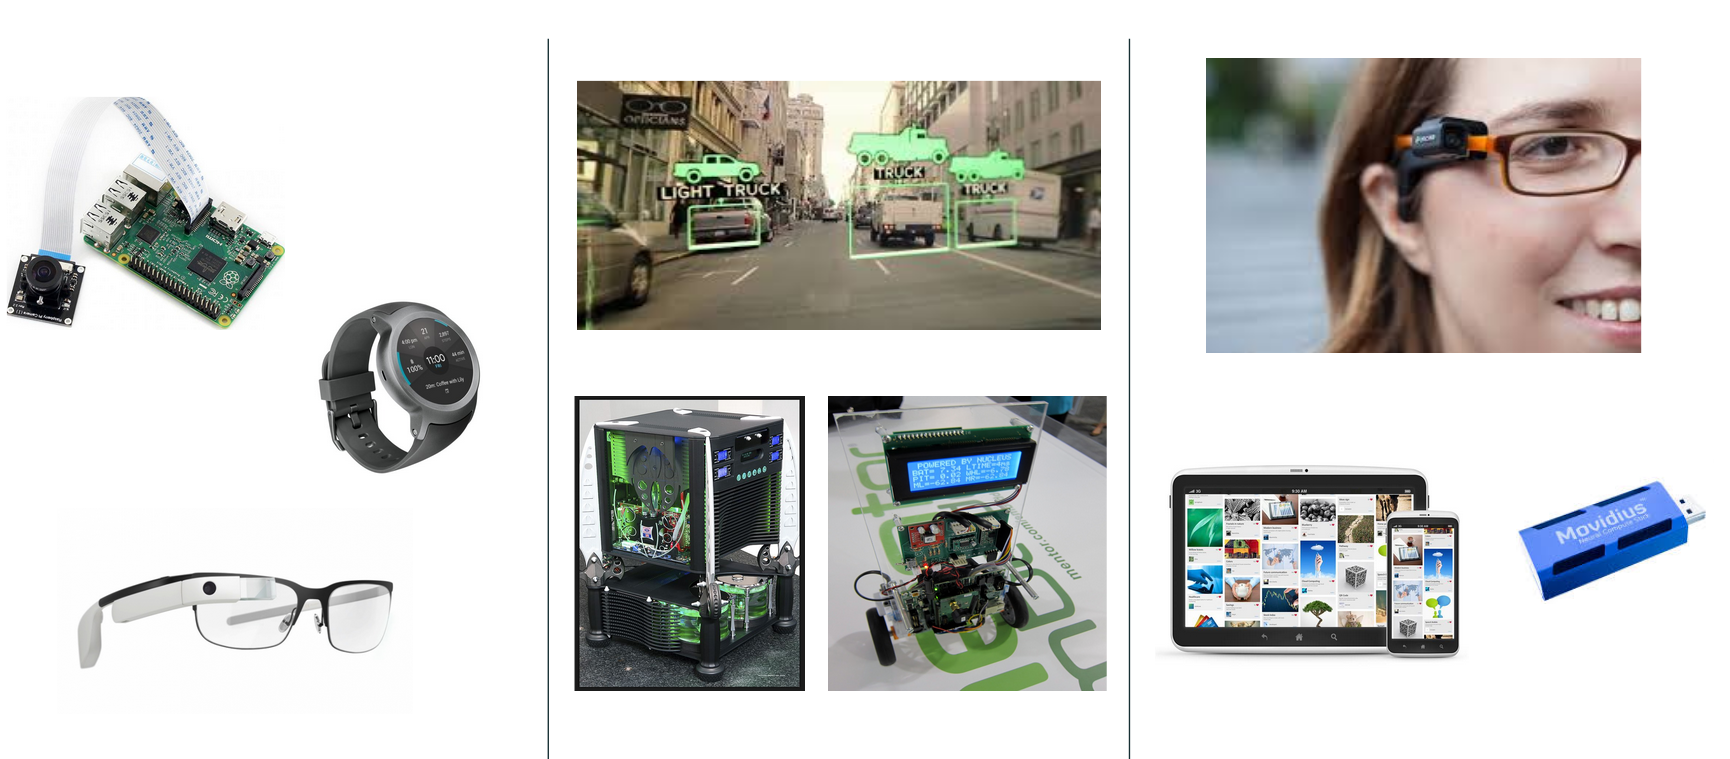
\includegraphics[width=0.9\textwidth]{figures/challenges.png}
\caption{There are two significant roadblocks to efficient deployment of large CNN models: realtime computation, and in-memory compactness. Cloud is not an option due to these real-time operation constraints.}
\label{fig:challenges}
%\vspace{-1.5cm}
\end{figure*}

\noindent Convolutional Neural Networks (CNNs) have found applications in many vision-related domains ranging from generic image-understanding for self-driving cars \cite{bojarski2016end} and automatic image captioning \cite{you2016image,johnson2016densecap} to recognition of specific image parts for scene-text recognition \cite{mishra2012top,neumann2012real} and face-based identification \cite{taigman2014deepface}. 

\noindent In the domain of image classification, AlexNet \cite{alex2012alexnet} and several architectural improvements  such as VGG-Net \cite{simonyan2014very} were proposed to push the limits of accuracy. These models were massive both in terms of memory usage and computational costs. AlexNet has around 60 million parameters in the network, while VGG has around 138 million, requiring 1.5 billion FLOPs and 19.6 billion FLOPs respectively for inference. The computational requirements make these architectures inappropriate for smaller portable systems such as mobiles and other embedded systems. These networks also consume large amounts of energy, creating a bottleneck for performance improvements. Full-precision multiply-accumulate (MAC) operations in floating point convolutional layers, for example, consumed 30x more power than integer MAC operations (see Table \ref{table:mac-energy}). These issues are addressed in two ways: (i) developing new compressed architectures (ii) compressing a given architecture.

\noindent There have been many developments in the area of model compression in the last few years, with the aim of bringing down runtimes and storage requirements to alleviate these challenges. Compression strategies for convolutional neural networks include architectural improvements \cite{he2016deep, iandola2016squeezenet}, reparametrization of fully connected layers \cite{moczulski2015acdc, yang2015deep}, pruning techniques \cite{han2015deep, liu2017learning}, and quantization \cite{courbariaux2016binarized, zhou2016dorefa}. Among these approaches, binarization and pruning  provided the most compact models as shown in Table \ref{table:versions_typesofcompression}. In this chapter, we motivate our exploration of binarization and pruning of convolutional neural networks, provide a background of methods explored in the past, and state the concrete contributions made in this thesis. 
 
\begin{table}[t]
\centering
\begin{tabular}{|l|c|}
\hline
{\bf Method} &  {\bf Compression} \\
\hline
Finetuned SVD 2 \cite{yang2015deep} & 2.6x \\
Circulant CNN 2 \cite{cheng2015exploration} & 3.6x \\
Adaptive Fastfood-16 \cite{yang2015deep} & 3.7x \\
Collins \etal \cite{collins2014memory} & 4x \\
Zhou \etal \cite{zhou2016less} & 4.3x \\
ACDC \cite{moczulski2015acdc} & 6.3x \\
Network Pruning \cite{han2015deep} & 9.1x \\
Deep Compression \cite{han2015deep} & 9.1x \\
GreBdec \cite{yu2017compressing} & 10.2x \\
Srinivas \etal \cite{srinivas2017training} & 10.3x \\
\hline
{\bf Guo \etal \cite{guo2016dynamic}} & {\bf 17.9x} \\
{\bf Binarization} & {\bf ${\approx}$32x} \\ 
\hline
\end{tabular}
\caption{Comparison of Binarization and other methods in terms of compression.}
\label{table:versions_typesofcompression}
\end{table}

\section{Quantization}

\noindent Quantized networks are networks where weights/activations are quantized into low-precision representations. These techniques achieve the best model compression and several promising directions have been explored in this domain  \cite{han2015deep}. They are classified into the categories based on the following questions:
\begin{enumerate}
\item How do they approximate the floating point values? 
\item Which part of the network do they quantize?
\end{enumerate}  

\noindent Weights are mainly appproximated by two broad methods: deterministic rounding and stochastic rounding. In deterministic rounding, there is an one-to-one mapping between the quantized value and the real value, while in stochastic quantization, there is a sampling distribution which assigns the quantized value. We constrain ourselves to deterministic rounding in this work, primarily due to it being implementable in hardware. There are two parts of a network which are targets of quantization: weights and activations. We take both steps, quantizing weights and activations to achieve compact models and lower computational cost.\\

\noindent Quantization has proven to be a powerful compression strategy, especially in its most extreme form: binarization. Binarization has enabled the use of XNOR-Popcount operations for vector dot products, which take much less time than full-precision Multiply-Accumulates (MACs), contributing to a huge speedup in convolutional layers \cite{rastegari2016xnor,courbariaux2016binarized} on a general-purpose CPU. Moreover, as each binary weight requires only a single bit to represent, one can achieve drastic reductions in run-time memory requirements. Previous research \cite{rastegari2016xnor,courbariaux2016binarized} shows that it is possible to perform weight and activation binarization on large networks with up to 58x speedups and approximately 32x compression ratios, albeit with significant drops in accuracy \cite{rastegari2016xnor}. Later works moved away from binary representations of weights/inputs to multi-bit representations. The reason for this was mainly the large accuracy drops observed in binary networks. \\
\begin{table}[t]
\begin{center}
\begin{tabular}{|l|c|c|c|c|}
\hline
{\bf Operation} & {\bf MUL} & {\bf Power} & {\bf ADD} & {\bf Power}\\ 
\hline
32-bit Float & 3.7pJ & 18.5x & 0.9pJ & 30x \\
16-bit Float & 1.1pJ & 5.5x & 0.4pJ &  13.3x\\
8-bit Integer & 0.2pJ & 1x & 0.03pJ & 1x \\
\hline
\end{tabular}
\end{center}
\caption{As shown by Horowitz \etal\cite{horowitz2014power}, power consumption for various operations at 45nm 0.9V. Observe that 8-bit integers require significantly less energy than their equivalent 32-bit floating point operations.}
\label{table:mac-energy}
\end{table}

 
\noindent  This leads to the natural question of whether, in theory, binary-representations of neural networks can be used at all to effectively approximate a full-precision network. If shown to be sufficient, the search for an accurate binarization technique is worthwhile, due to the large gains in speedups (due to binary operations rather than full-precision MACs) and compression compared to multi-bit representations. We also offer intuitions about how this technique might be effective in problems involving data that is binary in nature, such as sketches.\\ 
 
\noindent We then explore the problem of hybrid binarization of a network. We propose a technique devised from our investigation into the question as to {\it where and which quantities of a network should one binarize}, with respect to inputs to a layer -- to the best of our knowledge, this is the first work that explores this question. We observe that in a trained fully binarized model, binarization leads to minimal error in some layers and significant errors in others. Our proposed partition algorithm, when run on trained fully binarized models can design effective architectures. When these hybrid models are trained from scratch, they  achieve a balance between compression, speedup, energy-efficiency, and accuracy. We conduct extensive experiments applying our method to different model architectures on popular large-scale classification datasets over different domains. The resulting models achieve significant speedups and compression with significant accuracy improvements over a fully binarized network.

\section{Compact layers (Pruning)}

\noindent Network pruning is widely used technique for reducing the inference cost of deep  models  in  low-resource  settings.  A  typical  pruning  algorithm  is  a  three stage pipeline,  i.e.,  training  (a  large  model),  pruning  and  finetuning.   During  pruning, according to a certain criterion, redundant weights are pruned and important weights are kept to preserve the accuracy. All commonly used pruning techniques center around exploiting the sparsity in neural networks. A byproduct of pruning is that it removes redundancies during retraining, helping to prevent overfitting.\\

\noindent On the other hand, developing a compact layer for deep networks helps save memory and computational costs. Architectures such as ResNet \cite{he2016deep}, DenseNet \cite{huang2017densely} significantly reduced model size compared to VGG-Net by proposing a bottleneck structure to reduce the number of parameters while improving speed and accuracy. Additionally, they directed the focus of efficient designs of convolutional layers on increasing connectivity. Additional connectivity with residual connections to previous layers provided efficient information flow through the network, enabling them to achieve an order of magnitude reduction in storage and computational requirements. We take inspiration from these approaches, to focus on designing highly connected networks. We explore making networks efficient by designing sparse networks that preserve connectivity properties. \\

\noindent Recent architectures like MobileNet\cite{howard2017mobilenets} improves the efficiency by an order of magnitude over a ResNet. However, in order to achieve this, they sparsify a network by removing several connections from a trained network, reducing their accuracies in the process. We ask a basic question: If we try to maximize the connectivity properties and information flow, can we achieve the same efficiency gains with minimal loss in accuracy? It is essential that the connections allow information to flow through the network easily. That is, each output node must at least have the capacity to be sensitive to features of previous layers. Traditional model compression techniques such as pruning can aggravate the problem, since they can prune the neuron connections of a layer, while being agnostic of global connectivity of the network. A necessary condition for having good representational power is efficient information flow through the network, which is particularly suited to be modeled by graphs. \\

\noindent We propose to make the connections between neurons (filters in the case of CNNs) according to specific graph constructions known as expander graphs. They have been widely studied in spectral graph theory \cite{spielman2007spectral} and pseudorandomness \cite{salil2012pseudo}, and are known to be sparse but highly connected graphs. Expander graphs have a long history in theoretical computer science, also being used in practice in computer networks, constructing error correcting codes, and in cryptography (for a survey, see \cite{hoory2006expander}). 

\section{Contributions}

Overall, in this thesis we make the following contributions: 
\begin{enumerate}
\item Binarization
\begin{enumerate}
\item We show that binary representations are as expressive as full precision neural networks for polynomial functions, and offer theoretical insights into the same. 
\item We present a generalized, distribution-aware representation for binary networks, and proceed to calculate the generalized parameter-values for any binary network. We offer an intuitive analysis and comparison of our representation vis-a-vis existing representations.
\item We provide a provably efficient implementation of networks trained using this representation. We demonstrate the effectiveness of our method by extensive experiments applying it to popular model architectures on large-scale sketch datasets and improving upon existing binarization approaches.
\item We propose a metric to jointly optimize binarization-errors of layers and the associated computational costs and a partitioning algorithm to find suitable layers for input binarization, based on the above metric, which generates hybrid model architectures which if trained from scratch, achieve a good balance between compression, speedup, energy-efficiency, and accuracy.
\item Insights into what the algorithm predicts, which can provide an intuitive framework for understanding why binarizing certain areas of networks demonstrably achieves significant compression with respect to other compression methods; with hybrid model architectures for AlexNet, ResNet-18, Sketch-A-Net and SqueezeNet with over 5-8\% accuracy improvements on various datasets like Imagenet and TU-Berlin sketch recognition;
\end{enumerate}
\item Pruning (Compact Layer Design)
\begin{enumerate}
\item We propose to represent neuronal connections in deep networks using expander graphs (see Section \ref{sec:approach}). We further prove that X-Nets have strong connectivity properties (see Theorem \ref{thm:conn}).
\item We provide memory-efficient implementations of  Convolutional (X-Conv) layers using sparse matrices and propose a fast expander-specific algorithm and empirically compare X-Conv layers with grouped convolutions that have the same level of sparsity but worse connectivity. X-Conv layers obtain a 4\% improvement in accuracy when both the techniques are applied to the MobileNet architecture trained on Imagenet (see Section \ref{sec:group}).
\item We demonstrate the robustness of our approach by obtaining better performance trade-offs when applied to some of the state of the art models like DenseNet-BC and ResNet with a simple design, additionally achieving comparable compression rates to even the state-of-the-art trained pruning techniques.
\item Since we enforce the sparsity before the training phase itself, our models are inherently compact and faster to train compared to pruning techniques. We leverage this and showcase the performance of wider and deeper X-Nets. 
\end{enumerate}
\end{enumerate}

\noindent We shall be diving into the details of each contribution in chronological order in this thesis. The next chapter shall explore existing literature and pose our contributions in context and how the proposed contributions are novel.

%--------------------------------------------------------
\chapter{Related Work}
\label{ch:related}
\noindent CNNs have a large number of redundant parameters, increasing memory and computational cost. Since these applications would be deployed on resource-constrained systems, CNN compression is an important emerging area for research on vision applications \cite{courbariaux2016binarized,zhou2016dorefa, han2015deep, liu2017learning, moczulski2015acdc, yang2015deep, he2016deep, iandola2016squeezenet}. In this chapter, we briefly point out the two areas which are similar to our work and mention some of the important contributions made in network compression literature. They are categorized as follows: (i) Network Pruning (ii) Network Quantization. We also describe hardware accelerators  available for quantized networks to tie-in with some proposed algorithms. We detail approaches like efficient network design and using low-rank approximations to reduce the  number of parameters of a network. A detailed overview of approaches to network compression can be found in surveys such as \cite{cheng2018recent, sze2017efficient}.
 
\section{Network Pruning} 

\noindent Some of the earliest work in network pruning were optimal brain damage \cite{lecun1990optimal} and optimal brain surgeon \cite{hassibi1993optimal} used a function of the Hessian matrix of the loss function to prune a network by reducing the number of connections. With the recent sucess of deep learning, network pruning methods have risen to prominence. Weight-level pruning has the highest compression rate while filter-level pruning is easier to practically exploit , with compression rates not far behind the former. Hence, filter-level pruning is currently considered superior \cite{liu2017learning}. 

\subsection{Pixel and Vector Pruning}

\noindent Optimal brain damage and optimal brain surgeon both belonged to this category. They pruned individual parameters of a network. The problem of pruning weights during train-time have been extensively studied in the literature \cite{sze2017efficient}. Deep compression \cite{han2015learning} also used pruning to achieve compression by an order of magnitude in various standard neural networks. SSL \cite{wen2016structured} regularizes filter values and shapes, along with depth structures. It also performs structured pruning in a channel-wise and filter-wise manner. Dynamic network surgery \cite{guo2016dynamic} builds upon these methods to incorporate connection splicing into pruning, implementing the pruning process in a dynamic way and achieving state-of-the-art compact networks.

\subsection{Channel and Filter Pruning}

\noindent Srinivas \etal \cite{srinivas2015data} propose a systematic data-free method to remove neurons instead of removing individual connections as above. Li \etal \cite{li2016pruning} removed entire filters in the network along with their connecting feature maps, reducing the computation costs significantly. ThiNet \cite{luo2017thinet} proposed to prune filters from a CNN to enable more efficient acceleration. He \etal \cite{he2017channel} propose an iterative two-step algorithm to effectively prune each layer, by a LASSO regression-based channel selection procedure for weights and minimize feature map errors by least square reconstruction.  Network slimming \cite{liu2017learning} proposed to zero out channels of inputs based on the scaling factor of the batch normalization layer as a measure of importance of each channel in the input.\\

\noindent Groupwise brain damage \cite{lebedev2016fast} prunes the convolutional kernel tensor in a group-wise fashion by adding group-level sparsity regularization to the standard training process. Group sparse regularization \cite{scardapane2017group} proposed a sparse group lasso penalty in order to impose group-level sparsity on the network’s connections. Group-level pruning has a practical speed-up which scales linearly with the sparsity level.

\section{Quantization}

\noindent There has been a major body of work that quantizes the networks at train-time to achieve efficiency, explored in the literature survey by Yunhui Guo \cite{guo2018survey}.

\subsection{Higher bit quantization}

\noindent HashedNets \cite{chen2015compressing} performed binning of network weights using hash functions. Deep compression \cite{han2015deep} introduced quantization into the current literature by employing trained quantization and Huffman coding to reduce the non-runtime memory from Han \etal \cite{han2015learning}. Zhou \etal \cite{zhou2017inq} quantized networks to 4-bit weights, achieving 8x memory compression by using 4 bits to represent 16 different values and 1 bit to represent zeros. Trained ternary quantization \cite{zhu2016trained} uses 2-bit weights and scaling factors to compress the model by 16x with little accuracy degradation.  Ternary weight networks \cite{li2016ternary} optimize a threshold-based ternary function for approximation, with stronger expressive abilities than binary networks.  The above works are limited in the sense that they cannot leverage most speedups obtained by quantization since general purpose hardware supports only 8-bit integers or 1-bit booleans. Binary networks, on the other hand gain speedups by \texttt{xnor-popcount} operations which could be performed on dedicated hardware. Similarly, they can be practically compressed by using the existing boolean datatype.

\subsection{1-bit quantization}

\noindent BinaryConnect \cite{courbariaux2015binaryconnect} was one of the first works to use binary (+1, -1) values for network parameters, achieving significant compression. Binary neural networks \cite{courbariaux2016binarized} quantized weights and activations of neural networks and achieved near full-precision accuracies for datasets like MNIST, SVHN and CIFAR10. Quantized neural networks\cite{hubara2017quantized} use low-precision quantized weights and inputs and replace floating-point arithmetic operations with bit-wise ones. XNOR-Nets \cite{rastegari2016xnor} followed the work of BNNs \cite{hubara2017quantized}, binarizing both layer weights and inputs and multiplying them with scaling constants - bringing significant accuracy improvements. DoReFa-Net \cite{zhou2016dorefa} used low bit-width gradients during backpropagation, and obtained train-time speedups. HWGQ-Net \cite{cai2017deep} introduces a better suited activation function substituting sign function for better training of quantized networks.  Recent research has proposed a variety of additional methods: including novel activation functions \cite{cai2017deep}, fixed-point bit-width allocations \cite{lin2016fixed}, etc. HTCBN \cite{tang2017train} introduce helpful techniques such as replacing ReLU layers with PReLU layers and a scale layer to recover accuracy loss on binarizing the last layer. Hou \etal \cite{hou2016loss} use Hessian approximations to minimize loss w.r.t. binary weights during training. Anderson \etal \cite{anderson2017high} offer a theoretical analysis of the workings of binary networks in terms of high-dimensional geometry.\\

\noindent Merolla \etal \cite{merolla2016deep} show that binary networks during testing exhibit a remarkable robustness to distortions beyond quantization, including additive and multiplicative noise, and a class of non-linear projections. Further works have extended this in various directions, including using local binary patterns \cite{juefei2016local} which proposed an LBC layer, comprising of a set of fixed sparse pre-defined binary convolutional filters that are not updated during the training process. Lookup-based compression methods \cite{bagherinezhad2016lcnn} extended that by encoding convolutions by few lookups to a dictionary that is trained to cover the space of weights in CNNs - with training jointly learning a dictionary and a small set of linear combinations of the it.

\section{Other network compression approaches}

\noindent We cover several other aspects explored in the network compression literature, such as low-rank approximations, efficient network architecture design for image recognition and other tasks like sketch recognition. 

\subsection{Low-rank Approximations} 

\noindent Several methods since \cite{sainath2013low} have been introduced to compress pretrained networks as well as train-time compression by approximation weight matrices by their low-rak approximations \cite{novikov2015tensorizing, masana2017domain}. \cite{jaderberg2014speeding} approximate a learnt full rank filter bank as combinations of a rank-1 filter basis ($w∗h$ into $w∗1$ and $1∗h$ filters). Denil \etal \cite{denil2013predicting} use a low-rank approximation using SVD to reduce the network redundancy.  \cite{kim2015compression} used Tucker decomposition method to get the low-rank approxmation. \cite{lebedev2014speeding} developed a low-rank CP-decomposition of the 4D convolution kernel tensor into a sum of a small number of rank-one tensors using non-linear least squares to replace the original layer.

\subsection{Sketch Recognition}

\noindent Works before \cite{yu2015sketch} did not lead to good results by applying image classification architectures, since they are better suited to images than sketches \cite{yu2015sketch}. Sketches require specialized, fine-tuned networks since they have significantly different characteristics as compared to images. Sketch-a-Net from Yu \etal. \cite{yu2015sketch, yu2017sketch} took these factors into account, and proposed a carefully designed network structure that suited sketch representations. Their model showed tremendous increments over the then state-of-the-art, and managed to beat the average human performance using late and early fusion of ensembles. This model has been adopted by a number of later works such as Bui \etal. \cite{bui2016sbir}, Yu \etal \cite{yu2016shoe}, Wang \etal \cite{wang2016crossir}.

\subsection{Efficient Architecture Design}

\noindent Currently there is extensive interest in developing novel convolutional layers/blocks and effectively leveraging them to improve architectures like \cite{iandola2016squeezenet, howard2017mobilenets, hu2017squeeze}. In contrast, approaches like \cite{szegedy2015going} try to design the macro-architectures by connecting pre-existing blocks. Recent concurrent work has been on performing architecture searches effectively \cite{liu2017hierarchical, zoph2017learning,zhong2017practical, liu2017progressive}. Our work is complementary to architecture search techniques as we can leverage their optimized macro-architectures.\\

\noindent Another line of efficient architecture design is grouped convolutions, first proposed in AlexNet\cite{alex2012alexnet} and popularized by MobileNets\cite{howard2017mobilenets} and XCeption\cite{chollet2017xception} architectures .  \cite{zhang2018shufflenet, sandler2018inverted, huang2018condensenet} are the latest works in this area.\\

\noindent It is interesting to note that recent breakthroughs in designing accurate deep networks \cite{he2016deep, huang2017densely} were made by introducing additional connectivity to enable the efficient flow of information through deep networks. This enables the training of compact, accurate deep networks. These approaches, along with grouped convolutions are closely related to our approach. 

\section{Novelty}

\noindent We  ask  the question:  Do  CNNs  need  the  representational power of 32-bit floating point operations? Is it possible to cut down memory costs and make output computations significantly less expensive? Previous literature performed binarization independent of the distribution weights. In Chapter 3, we introduce distribution-aware binarization method which depends on the distribution of weights to calculate an optimal binarization.\\

\noindent Unlike previous work in this area, we look at binarizing specific parts of a network, instead of simply binarizing the inputs to all the layers end-to-end. We see in Chapter 4, binarizing the right areas in the network contributes significantly to the overall accuracy of the network without compromising on speed-ups.\\

\noindent To the best of our knowledge, the method we propose in Chapter 5 is the first attempt at constraining neural network connections by graph-theoretic approaches to improve deep network architecture designs. We differ from previous work by not pruning weights during training, and still achieve comparable performance.

%--------------------------------------------------------
\chapter{Distribution Aware Binarization of Networks}
\label{ch:dabn}

\noindent In this chapter, we will explore the first question: How to form a distribution aware method of compressing binary neural networks. As illustrated in Figure \ref{fig:alphabetadiagram} that changes in the binarization function can influence it's ability to detect portions of an image more accurately.

\begin{figure}[h]
\centering
           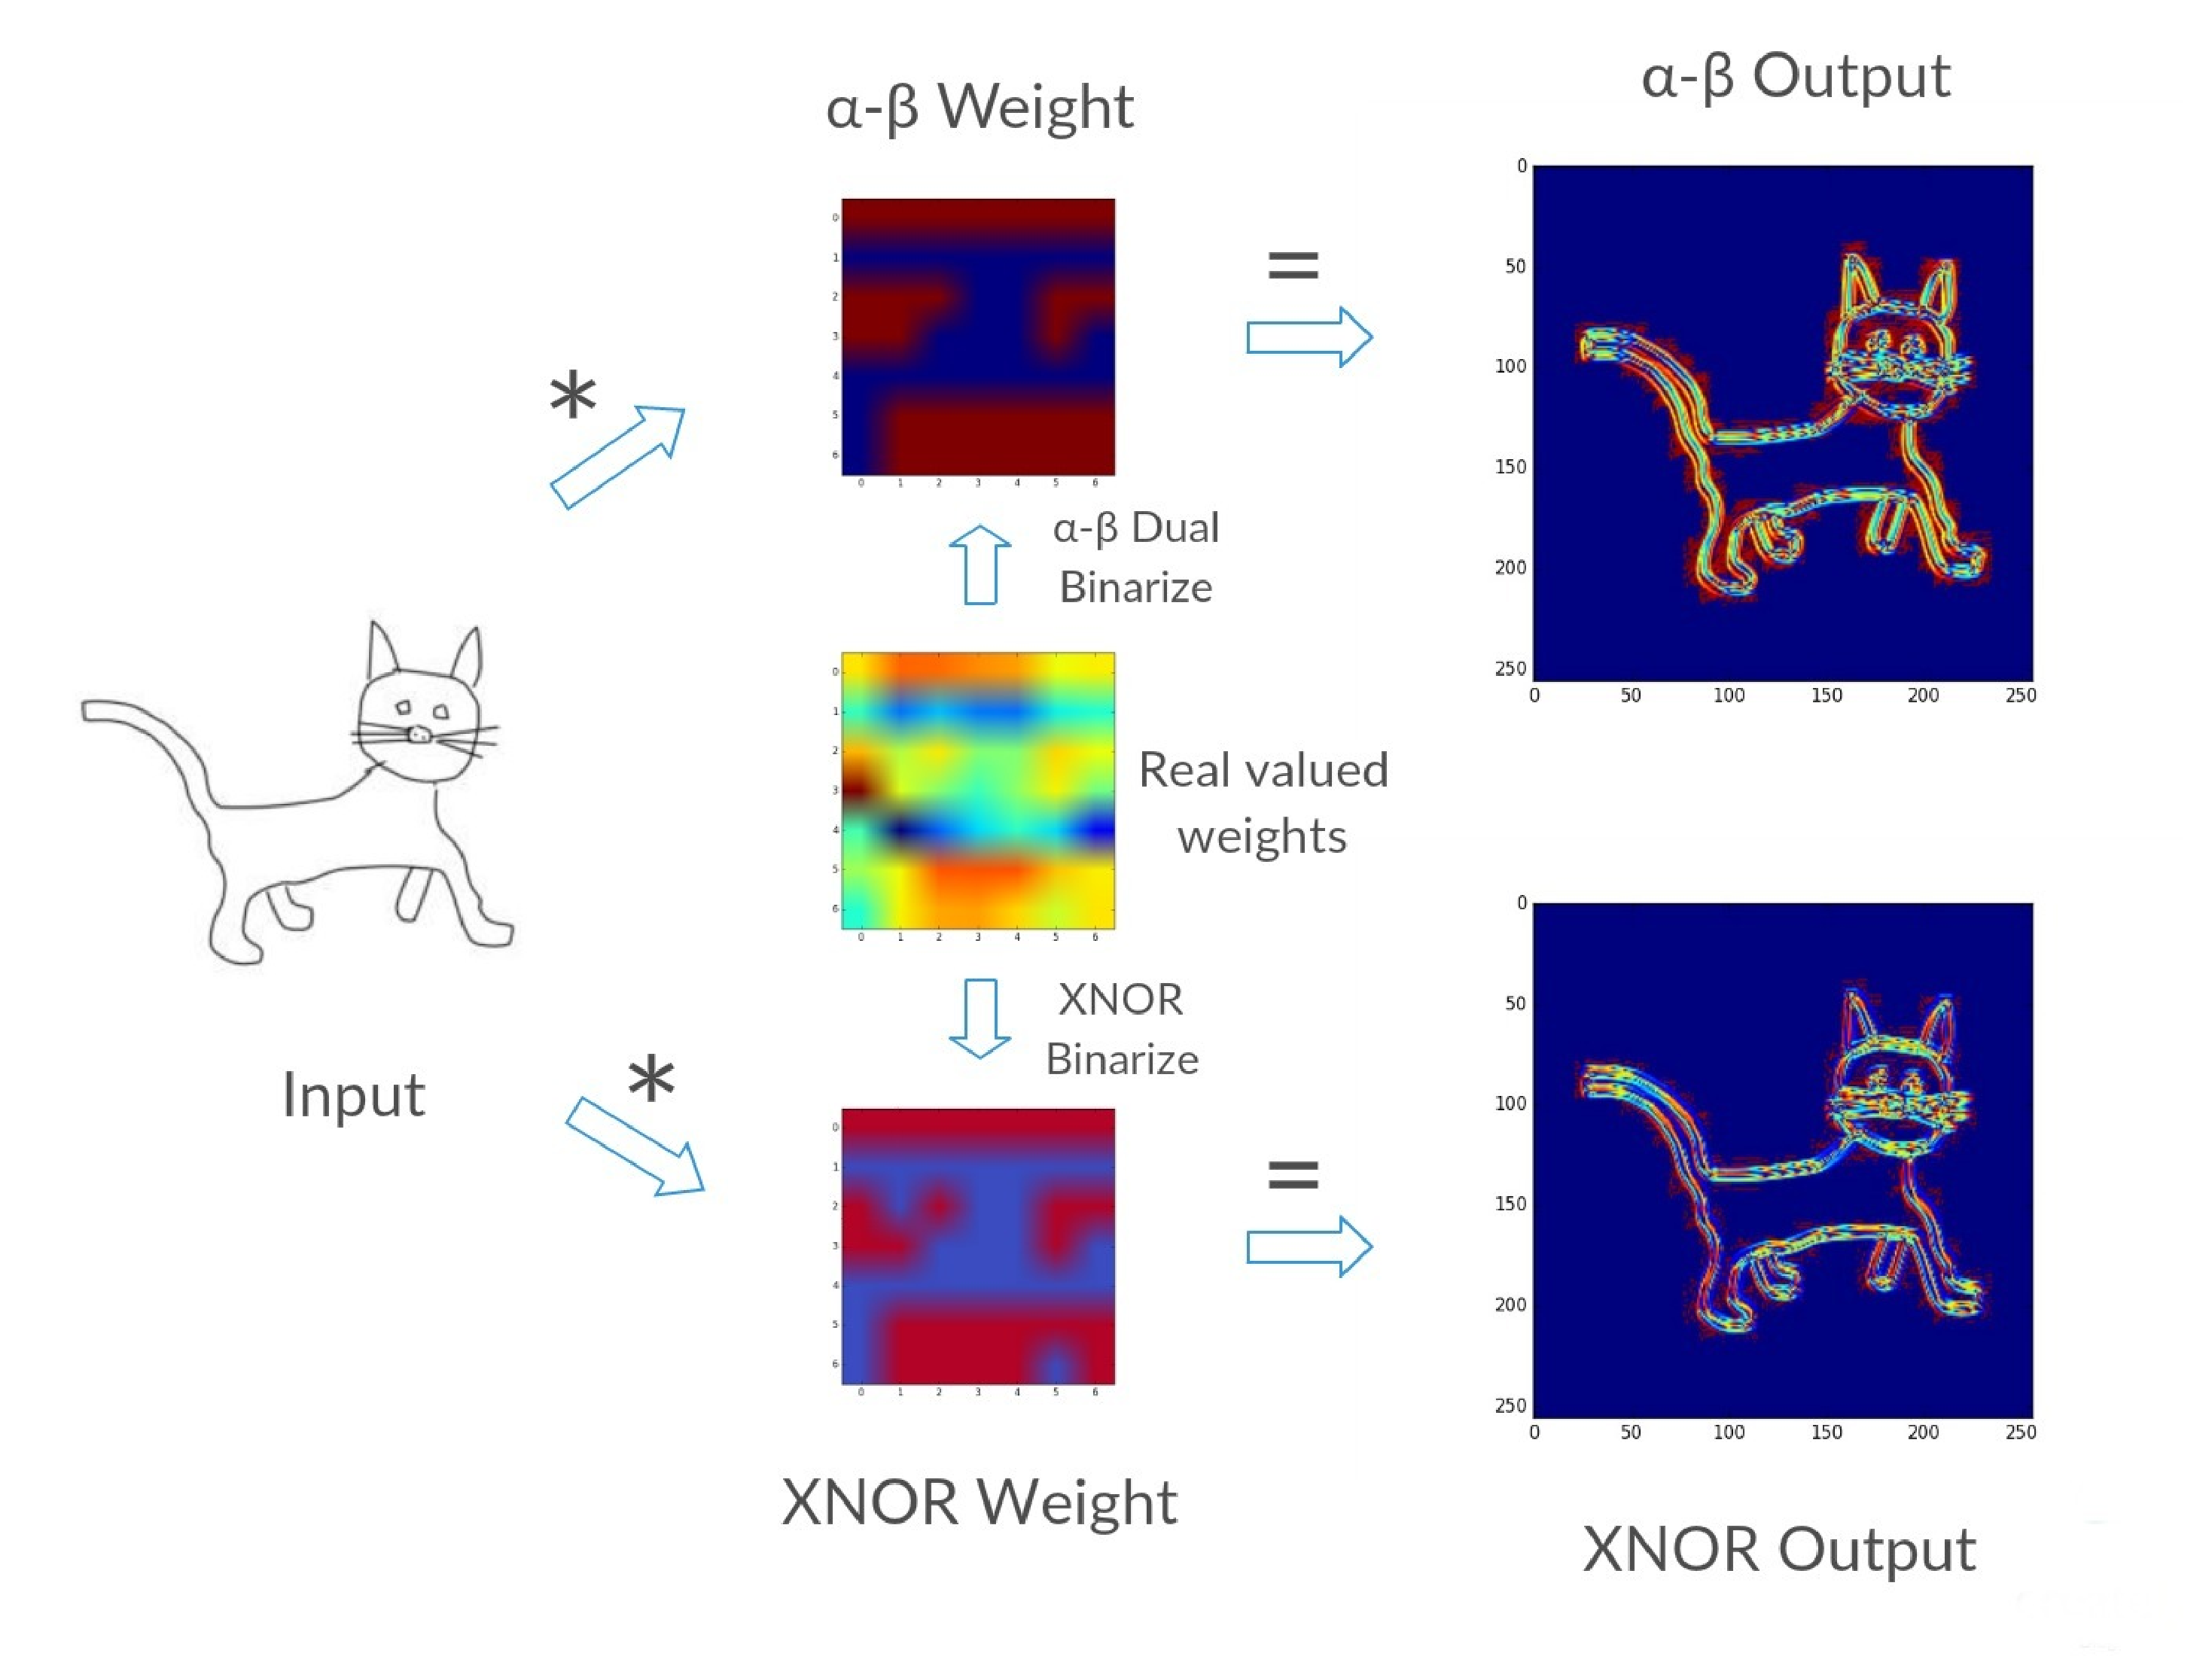
\includegraphics[width=0.45\textwidth]{figures/MainDiagram-CVPR.pdf}
           \caption{An example sketch passing through a convolutional layer filter, with the real-valued filter shown alongside corresponding $\alpha$-$\beta$ and XNOR-Net filters. Orange signifies the highest response areas. We can see that DAB-Net has significantly better responses when compared to XNOR-Net}
        \label{fig:alphabetadiagram}
\end{figure}

\section{Representational Power of Binary Networks} 

\noindent Many recent works in network compression involve higher bit weight quantization using two or more bits \cite{zhou2017inq,li2016ternary,li2016ternary} instead of binarization, arguing that binary representations would not be able to approximate full-precision networks. In light of this, we explore whether the representational power that binary networks can offer is theoretically sufficient to get similar representational power as full-precision networks.\\

\noindent Rolnick \etal \cite{lin2017does,rolnick2017power} have done extensive work in characterizing the expressiveness of neural networks. They claim that due to the nature of functions - that they depend on real-world physics, in addition to mathematics - the seemingly huge set of possible functions could be approximated by deep learning models. From the Universal Approximation Theorem \cite{cybenko1989approximation}, it is seen that any arbitrary function can be well-approximated by an Artificial Neural Network; but \textit{cheap learning}, or models with far fewer parameters than generic ones, are often sufficient to approximate multivariate monomials - which are a class of functions with practical interest, occurring in most real-world problems.\\

\noindent We can define a binary neural network having $k$ layers with activation function $\sigma(x)$  and consider how many neurons are required to compute a multivariate monomial $p(x)$ of degree $d$. The network takes an $n$ dimensional input $\mathbf{x}$, producing a one dimensional output $p(x)$. We define $B_k(p,\sigma)$ to be the minimum number of binary neurons (excluding input and output) required to approximate $p$, where the error of approximation is of degree at least $d+1$ in the input variables. For instance, $B_1(p,\sigma)$ is the minimal integer $m$ such that:
$$\sum_{j=1}^m w_j \sigma\left(\sum_{i=1}^n a_{ij} x_i\right) = p(x) + \mathcal{O}(x_1^{d + 1} + \ldots + x_n^{d + 1}).$$ 
Any polynomial can be approximated to high precision as long as input variables are small enough \cite{lin2017does}. Let $B(p, \sigma) = \min_{k \geq 0} B_k(p, \sigma)$.

\begin{theorem}
\label{theorem:binaryrepresentation}
For $p(\mathbf{x})$ equal to the product $x_1x_2\cdots x_n$, and for any $\sigma$ with all nonzero Taylor coefficients, we have one construction of a binary neural network which meets the condition
\begin{equation}
B_k(p, \sigma) = \mathcal{O}\left(n^{(k-1)/k}\cdot 2^{n^{1/k}}\right).\label{eqn:constantlayers}
\end{equation}

Proof of the above can be found in the appendix A. 
\end{theorem}

\noindent Conjecture III.2. of Rolnick \etal \cite{rolnick2017power} says that this bound is approximately optimal. If this conjecture is true, weight-binarized networks would have the same representational  power as full-precision networks, but with finite (1-bit) precision. Another case would be 2 layer network, where we can say a binary network requires the same number of neurons as a full-precision network, $2^n$. 

\begin{theorem}
For any desired accuracy $\epsilon>0$, there exists a binary neural network $B_1(p,\sigma)$ that can compute the function $p(x)$ using a single hidden layer of $2^n$ binary-weighted neurons.

Proof of the above can be found in the appendix A.
\end{theorem}

\noindent The above theorem shows that any neural network that can be represented as a multivariate polynomial function is considered as a simplified model with ELU-like activations, using continuously differentiable layers - so pooling layers are excluded as well. While there can exist a deep binary-weight network that can possibly approximate polynomials similar to full precision networks, it does say that such a representation would be efficiently obtainable through Stochastic Gradient Descent. Also, this theorem assumes only weights are binarized, not the activations. Activation binarization typically loses a lot of information and might not be a good thing to do frequently. However, this insight motivates the fact that more investigation is needed into approximating networks through binary network structures.

\section{Distribution-Aware Binarization}

\noindent We have so far established that binary representations are possibly sufficient to approximate a polynomial with similar numbers of neurons as a full-precision neural network. We now investigate the question - What is the most general form of binary representation possible? In this section, we derive a generalized distribution-aware formulation of binary weights, and provide an efficient implementation of the same. We consider models binarized with our approach as DAB-Nets (Distribution Aware Binarized Networks).\\

\noindent We model the loss function layer-wise for the network. We assume that inputs to the convolutional layers are binary - i.e. belong to $\{+1, -1\}$, and find constants $\alpha$ and $\beta$ (elaborated below) as a general binary form for layer weights. These constants are calculated from the distribution of real-valued weights in a layer - thus making our approach \textit{distribution-aware}. 

\subsection{Derivation}
\noindent Without loss of generality, we assume that $\mathbf{W}$ is a vector in $R^{n}$ , where $n = c\cdot w\cdot h$.
We attempt to binarize the weight vector $\mathbf{W}$ to $\widetilde{\mathbf{W}}$ which takes a form similar to this example - $[\alpha \alpha... \beta \alpha \beta]$. Simply put, $\widetilde{\mathbf{W}}$ is a vector consisting of scalars $\alpha$ and $\beta$, the two values forming the binary vector. We represent this as $\widetilde{\mathbf{W}} = \alpha \mathbf{e} + \beta \mathbf{(1-e)}$ where $\mathbf{e}$ is a vector such that $\mathbf{e} \in \{0,1\}^n \ni \mathbf{e} \neq 0$ and $\mathbf{e} \neq 1$.  We define $K$ as $\mathbf{e}^T\mathbf{e}$ which represents the number of ones in the $\mathbf{e}$ vector. Our objective is to find the best possible binary approximation for $\mathbf{W}$. We set up the optimization problem as: $$\widetilde{\mathbf{W}}^\ast = \underset{\widetilde{\mathbf{W}}}{\mathrm{argmin}}\mid\mid \mathbf{W}-\widetilde{\mathbf{W}}\mid\mid^{2}$$ We formally state this as the following: \\

%\begin{theorem}
\label{approx}
{\it The optimal binary weight vector $\widetilde{\mathbf{W}}^\ast$ for any weight vector $\mathbf{\mathbf{W}}$ which minimizes the approximate-error function $\mathbf{J} = \mid\mid \mathbf{W}-\widetilde{\mathbf{W}}\mid\mid^{2}$ can be represented as: %in terms of scalar parameters $\alpha$, $\beta$ and vector $e$ as: 
$$\widetilde{\mathbf{W}}^\ast = \alpha \mathbf{e} + \beta \mathbf{(1-e)}  \; where\\$$
$$ \alpha =\frac{\mathbf{W}^{T}\mathbf{e}}{K} \;, \; \beta = \frac{\mathbf{W}^{T}\mathbf{(1-e)}}{n-K} $$ for a given $K$. That is, given a $K$, the optimal selection of $\mathbf{e}$ would correspond to either the $K$ smallest weights of $\mathbf{W}$ or the $K$ largest weights of $\mathbf{W}$. 

The best suited $K$, we calculate the value of the following expression for every value of $K$, giving us an $\mathbf{e}$, and maximize the expression: $$  \mathbf{e}^\ast  = \underset{\mathbf{e}}{\mathrm{argmax}}  (\frac{\mid\mid\mathbf{\mathbf{W}}^T\mathbf{e}\mid\mid^2}{K}+\frac{\mid\mid\mathbf{W}^T\mathbf{(1-e)}\mid\mid^2}{n-K}) \\$$
A detailed proof of the above can be found in the appendix A.}
\\\\
\noindent The above representation shows the values obtained for $\mathbf{e}$, $\alpha$ and $\beta$ are the optimal approximate representations of the weight vector $\mathbf{W}$. The vector $\mathbf{e}$, which controls the number and distribution of occurrences of $\alpha$ and $\beta$, acts as a mask of the top/bottom $K$ values of $\mathbf{W}$. We assign $\alpha$ to capture the greater of the two values in magnitude. Note that the scaling values derived in the XNOR formulation, $\alpha$ and $-\alpha$, are a special case of the above, and hence our approximation error is at most that of the  XNOR error. We explore what  this function represents and how this relates to previous binarization techniques in the next subsection.

\subsection{Intuitions about DAB-Net}

\noindent In this section, we investigate intuitions about the derived representation. We can visualize that $\mathbf{e}$ and $\mathbf{(1-e)}$ are orthogonal vectors. Hence, if normalized, $\mathbf{e}$ and $\mathbf{(1-e)}$ form a basis for a subspace $R^{2}$. Theorem 2 says the best $\alpha$ and $\beta$ can be found by essentially projecting the weight matrix $\mathbf{W}$ into this subspace, finding the vector in the subspace which is \textit{closest} to $\mathbf{e}$ and $\mathbf{(1-e)}$ respectively. $$\alpha = \frac{\langle \mathbf{W}, \mathbf{e} \rangle}{\langle \mathbf{e} , \mathbf{e} \rangle} \cdot \mathbf{e} \ , \  \beta = \frac{\langle \mathbf{W}, \mathbf{(1-e)} \rangle}{\langle \mathbf{(1-e)} , \mathbf{(1-e)} \rangle} \cdot \mathbf{(1-e)}$$ 

\noindent We also show that our derived representation is different from the previous binary representations since we cannot derive them by assuming a special case of our formulation. XNOR-Net \cite{rastegari2016xnor} or BNN \cite{courbariaux2016binarized}-like representations cannot be obtained from our formulation.

\subsection{Implementation}

\begin{algorithm}[t]
\caption{ Finding an optimal K value. }
\begin{algorithmic}[1]
\State \texttt{Initialization}
\State $\mathbf{W}$ = 1D weight vector
\State $T$ = Sum of all the elements of $\mathbf{W}$
\State  Sort($\mathbf{W}$)
\State $D$ = $[0 0... 0]$ ~~//~{Empty array of same size as $\mathbf{W}$}
\State $optK_{1}$ = 0 ~~//~{Optimal value for K}
\State $maxD_{1}$ = 0 ~~//~{Value of D for optimal K value} \\

\For{$I$= 1 to D.size}
	\State $P_{i} = P_{i-1} + \mathbf{W}_{i}$
	\State $D_{i} = \frac{P_{i}^{2}}{i} + \frac{(T-P_{i})^{2}}{n-i}$
    \If{$D_{i} \geq maxD_{1}$}
    \State $maxD_{1}$ = $D_{i}$
    \State $optK_{1}$ = i
    \EndIf
\EndFor
\\
\State Sort($\mathbf{W}$, reverse=true) and {\bf Repeat} steps 4-13 with $optK_{2}$ and $maxD_{2}$
\\
\State $optK_{final}$ = $optK_{1}$
\If{$maxD_{2} > maxD_{1}$}
\State $optK_{final}$ = $optK_{2}$
\EndIf
\\
\State {\bf return} $optK_{final}$
\end{algorithmic}
\label{alg:partitionalgo}
\end{algorithm}

\noindent The representation that we earlier derived requires to be efficiently computable, in order to ensure that our algorithm runs fast enough to be able to train binary networks. In this section, we investigate the implementation, by breaking it into two parts: 1) Computing the parameter $K$ efficiently for every iteration. 2) Training the entire network using that value of $K$ for a given iteration. We show that it is possible to get an efficiently trainable network at minimal extra cost. We provide an efficient algorithm using Dynamic Programming which computes the optimal value for $K$ quickly at every iteration. \\

\subsubsection{Parallel Prefix-Sums to Obtain $K$}
\begin{theorem}
\label{theorem:approx}
The optimal $K^*$ which minimizes the value $\mathbf{e}$ can be computed in $O(n \cdot logn)$ complexity.
\end{theorem}

\noindent Considering one weight filter at a time for each convolution layer, we flatten the weights into a 1-dimensional weight vector $\mathbf{W}$. We then sort the vector in ascending order and then compute the prefix-sum array $P$ of $\mathbf{W}$. For a selected value of $K$, the term to be maximized would be $(\frac{\mid\mid\mathbf{\mathbf{W}}^T\mathbf{e}\mid\mid^2}{K}+\frac{\mid\mid\mathbf{W}^T\mathbf{(1-e)}\mid\mid^2}{n-K})$, which is equal to $(\frac{P_{i}^{2}}{i} + \frac{(T-P_{i})^{2}}{n-i})$ since the top $K$ values in $\mathbf{W}$ sum up to $P_{i}$ where $T$ is the sum of all weights in $\mathbf{W}$. We also perform the same computation with a descending order of $\mathbf{W}$'s weights since $K$ can correspond to either the smallest $K$ weights or the largest $K$ weights as we mentioned earlier. In order to speed this up, we perform these operations on all the weight filters at the same time considering them as a 2D weight vector instead. Our algorithm runs in $O(n \cdot logn)$ time complexity, and is specified in Algorithm \ref{alg:partitionalgo}. This algorithm is integrated into our code, and will be provided alongside.

\subsubsection{Forward and Backward Pass}
\noindent Now that we know how to calculate $K$, $\mathbf{e}$, $\alpha$, and $\beta$ for each filter in each layer optimally, we can compute $\widetilde{\mathbf{W}}$ which approximates $\mathbf{W}$ well. Here, $topk(\mathbf{W},K)$ represents the top $K$ values of $\mathbf{W}$ which remain as is whereas the rest are converted to zeros. Let $\mathbf{T_k} = topk(\mathbf{W}, K)$.

\begin{corollary}[Weight Binarization]\label{corollary:forward}
The optimal binary weight $\widetilde{\mathbf{W}}$ can be represented as,
\[
\widetilde{\mathbf{W}} = \alpha.sgn(\mathbf{T_k}) + \beta.(1-sgn(\mathbf{T_k}))
\]
where,
\[
\alpha = \frac{\mathbf{T_k}}{K} \ and \ 
\beta = \frac{(\mathbf{W}-\mathbf{T_k})}{n-K}
\]
\end{corollary}

\noindent Once we have $\widetilde{\mathbf{W}}$, we can perform convolution as $\bf{I} \circledast \widetilde{\mathbf{W}}$ during the forward pass of the network. Similarly, the optimal gradient $\widetilde{\mathbf{G}}$ can be computed as follows, which is back-propagated throughout the network in order to update the weights:

\begin{algorithm}[t]
{
  \caption{Training an $L$-layers CNN with binary weights:}
  \label{alg:trainbinconv}       
  \begin{algorithmic}[1]
  \State A minibatch of inputs and targets  ($\mathbf{I}, \mathbf{Y}$), cost function $C(\mathbf{Y},\hat{\mathbf{Y}})$, current weight $\mathbf{W}^t$ and current learning rate $\eta^t$.     
  \State updated weight $\mathbf{W}^{t+1}$ and updated learning rate $\eta^{t+1}$. 
  \State {\bf Binarizing weight filters}:
  \State $\mathbf{W}^t$ = MeanCenter($\mathbf{W}^t$)
  \State $\mathbf{W}^t$ = Clamp($\mathbf{W}^t$, -1, 1)
  \State $\mathbf{W}_{real}$ = $\mathbf{W}^t$
  \For{$l=1$ to $L$}
      \For{$j^{\text{th}}$ filter in $l^{\text{th}}$ layer}
      	  \State Find $K_{lj}$ using Algorithm \ref{alg:partitionalgo}
          \State $\alpha_{lj}=\frac{topk(\mathbf{W}_{lj},K_{lj})}{K_{lj}}$
          \State $\beta_{lj}=-\frac{(\mathbf{W}_{lj}-topk(\mathbf{W}_{lj},K_{lj}))}{n-K_{lj}}$
          \State $\widetilde{\mathbf{W}}_{lj}=\alpha.sgn(topk(\mathbf{W}_{lj},K_{lj}))$ \\ \ \ \ \ \ \ \ \ \ \ \ \ \ \ \ \ \ \ \ \ \ \ \  $ + \ \beta.(1-sgn(topk(\mathbf{W}_{lj},K_{lj})))$
      \EndFor
   \EndFor
   \\
   \State $\hat{\mathbf{Y}}=$ ~~\textbf{BinaryForward}$(\mathbf{I},\widetilde{\mathbf{W}})$
   \\
   \State $\frac{\partial C}{\partial \widetilde{\mathbf{W}}} =$ \textbf{BinaryBackward}$(\frac{\partial C}{\hat{\mathbf{Y}}}, \widetilde{\mathbf{W}})$ ~~//~{ Standard backward propagation except that gradients are computed using $\widetilde{\mathbf{W}}$ instead of $\mathbf{W}^t$} as mentioned in Theorem. \ref{theorem:backward}
   \\
 \State We then copy back the real weights in order to apply the gradients computed. $\mathbf{W}^t$ = $\mathbf{W}_{real}$ \\
 \State $\mathbf{W}^{t+1}$ = \textbf{UpdateParameters}$(\mathbf{W}^{t},\frac{\partial C}{\partial \widetilde{\mathbf{W}}}, \eta^t)$ 
 \State $\eta^{t+1}=$ \textbf{UpdateLearningrate}$(\eta^t, t)$
  \end{algorithmic}
}
\end{algorithm}

\begin{theorem}[Backward Pass]\label{theorem:backward}
The optimal gradient value $\widetilde{G}$ can be represented as,
\begin{dmath}
\widetilde{\mathbf{G}} = \widetilde{\mathbf{G_1}} + \widetilde{\mathbf{G_2}}
\end{dmath}
where,
\begin{dmath}
\widetilde{\mathbf{G_1}} = \frac{sgn(\mathbf{T_k})}{K}\circ sgn(\mathbf{T_k}) + \frac{||\mathbf{T_k}||_{l1}}{K} .STE(\mathbf{T_k})
\end{dmath}
\begin{dmath}
\widetilde{\mathbf{G_2}} = \frac{sgn(\mathbf{W}-\mathbf{T_k})}{n-K} \circ (1-sgn(\mathbf{T_k})) + \frac{||\mathbf{W}-\mathbf{T_k}||_{l1}}{n-K}.STE(\mathbf{W} - \mathbf{T_k})
\end{dmath}
\begin{equation}
STE(\mathbf{T_k})^{i} = 
    \begin{cases}
      \mathbf{T_k}^{i}, \text{where} \ |\mathbf{W}|^{i}<=1 \\
      0,\ \text{elsewhere}
    \end{cases}
\end{equation}
\end{theorem}

\noindent The gradient vector, as seen above, can be intuitively understood if seen as the sum of two independent gradients $\widetilde{\mathbf{G_1}}$ and $\widetilde{\mathbf{G_2}}$, each corresponding to the vectors $\mathbf{e}$ and $\mathbf{(1-e)}$ respectively. Further details regarding the derivation of this gradient would be provided in the supplementary material.

\subsection{Training Procedure}

\noindent Putting all the components mentioned above together, we have outlined our training procedure in Algorithm \ref{alg:trainbinconv}. During the forward pass of the network, we first mean center and clamp the current weights of the network. We then store a copy of these weights as $\mathbf{W}_{real}$. We compute the binary forward pass of the network, and then apply the backward pass using the weights $\widetilde{\mathbf{W}}$, computing gradients for each of the weights. We then apply these gradients on the original set of weights $\mathbf{W}^t$ in order to obtain $\mathbf{W}^{t+1}$. In essence, binarized weights are used to compute the gradients, but they are applied to the original stored weights to perform the update. This requires us to store the full precision weights during training, but once the network is trained, we store only the binarized weights for inference.

\section{Experiments}
\noindent We empirically demonstrate the effectiveness of our optimal distribution-aware binarization algorithm (DAB-Net) on the TU-Berlin and Sketchy datasets. We compare DAB-Net with BNN and XNOR-Net \cite{rastegari2016xnor} on various architectures, on two popular large-scale sketch recognition datasets as sketches are sparse and binary. Also, they are easier to train with than standard images, for which we believe the algorithm needs to be stabilized - in essence, the $K$ value must be restricted to change by only slight amounts. We show that our approach is superior to existing binarization algorithms, and can generalize to different kinds of CNN architectures on sketches.

\subsection{Experimental Setup}
\noindent In our experiments, we define the network having only the convolutional layer weights binarized as WBin, the network having both inputs and weights binarized as FBin and the original full-precision network as FPrec. Binary Networks have achieved accuracies comparable to  full-precision networks on limited domain/simplified  datasets like CIFAR-10, MNIST, SVHN, but show considerable losses on larger datasets. Binary networks are well suited for sketch data due to its binary and sparse nature of the data. \\

\noindent {\bf TU-Berlin:} The TU-Berlin \cite{eitz2012hdhso} dataset is the most popular large-scale free-hand sketch dataset containing sketches of 250 categories, with a human sketch-recognition accuracy of 73.1\% on an average.\\

\noindent {\bf Sketchy:} A recent large-scale free-hand sketch dataset containing 75,471 hand-drawn sketches spanning 125 categories. This dataset was primarily used to cross-validate results obtained on the TU-Berlin dataset, to ensure the robustness of our approach with respect to the method of data collection.\\

\noindent For all the datasets, we first resized the input images to 256 x 256. A 224 x 224 (225 x 225 for Sketch-A-Net) sized crop was then randomly taken from an image with standard augmentations such as rotation and horizontal flipping, for TU-Berlin and Sketchy. In the TU-Berlin dataset, we use three-fold cross validation which gives us a 2:1 train-test split ensuring that our results are comparable with all previous methods. For Sketchy, we use the training images for retrieval as the training images for classification, and validation images for retrieval as the validation images for classification. We report ten-crop accuracies on both the datasets.\\

\noindent We used the PyTorch framework to train our networks. We used the Sketch-A-Net\cite{yu2015sketch}, ResNet-18\cite{he2016deep} and GoogleNet\cite{szegedy2015going} architectures. Weights of all layers except the first were binarized throughout our experiments, except in Sketch-A-Net for which all layers except first and last layers were binarized.  All networks were trained from scratch. We used the Adam optimizer for all experiments. Note that we do not use a bias term or weight decay for binarized Conv layers. We used a batch size of 256 for all Sketch-A-Net models and a batch size of 128 for ResNet-18 and GoogleNet models, the maximum size that fits in a 1080Ti GPU. Additional experimental details are available in the supplementary material.

\begin{table}[t]  
\centering
\begin{tabular}{|l|c|c|c|}
\hline
\multirow{2}{*}{\bf Models} &  \multirow{2}{*}{\bf Method} &  \multicolumn{2}{c|}{\sc { \bf Accuracies}}\\
\cline{3-4}

 &   & TU-Berlin & Sketchy\\
\hline
\multirow{5}{*}{Sketch-A-Net} & FPrec  & 72.9\%  & 85.9\%\\
 & WBin (BWN)  & 73.0\% & 85.6\%\\
 & FBin (XNOR-Net) & 59.6\% & 68.6\% \\
 & WBin DAB-Net  & 72.4\% & 84.0\% \\
 & FBin DAB-Net  & {\bf 60.4\%} & {\bf 70.6\%} \\
\hline
Improvement & XNOR-Net vs DAB-Net & +0.8\% & +2.0\%\\
\hline
\multirow{5}{*}{ResNet-18} & FPrec & 74.1\% & 88.7\% \\
 & WBin (BWN) & 73.4\%  & 89.3\%\\
 & FBin (XNOR-Net) & 68.8\% & 82.8\%\\
 & WBin DAB-Net  & 73.5\% & 88.8\%\\
 & FBin DAB-Net  & {\bf 71.3\%} & {\bf 84.2\%}\\
\hline
Improvement & XNOR-Net vs DAB-Net & +2.5\% & +1.4\%\\
\hline
\multirow{5}{*}{GoogleNet} & FPrec & 75.0\% & 90.0\% \\
 & WBin (BWN) & 74.8\%  & 89.8\%\\
 & FBin (XNOR-Net) & 72.2\% & 86.8\% \\
 & WBin DAB-Net  & 75.7\% & 90.1\%\\
 & FBin DAB-Net  & {\bf 73.7\%} & {\bf 87.4\%} \\
\hline
Improvement & XNOR-Net vs DAB-Net & +1.5\% & +0.6\%\\
\hline
\end{tabular}
\caption{Our DAB-Net models compared to FBin, WBin and FPrec models on TU-Berlin and Sketchy in terms of accuracy.} 
\label{table:tub_recacc}
\end{table}
\begin{table}[t]
\begin{center}
\begin{tabular}{|l|c|c|c|l|}
\hline
{\bf Models}  &  {\bf Accuracy}\\
\hline
AlexNet-SVM  & 67.1\%\\
AlexNet-Sketch  & 68.6\%\\
Sketch-A-Net SC  & 72.2\%\\
Humans & {73.1\%}\\
Sketch-A-Net-2\footnotemark \cite{yu2017sketch} & {\bf 77.0\%}\\
\hline
Sketch-A-Net WBin DAB-Net & 72.4\%\\
ResNet-18 WBin DAB-Net & 73.5\%\\
GoogleNet WBin DAB-Net & {\bf 75.7\%}\\
\hline
Sketch-A-Net FBin DAB-Net & 60.4\%\\
ResNet-18 FBin DAB-Net & 71.3\%\\
GoogleNet FBin DAB-Net & {\bf 73.7\%}\\
\hline
\end{tabular}
\end{center}
\caption{A comparison between state-of-the-art single model accuracies of recognition systems on the TU-Berlin dataset.}
\label{table:sketchcomp}
\end{table}
\begin{figure*}[t]
\begin{center}
\begin{tabular}{cc}
           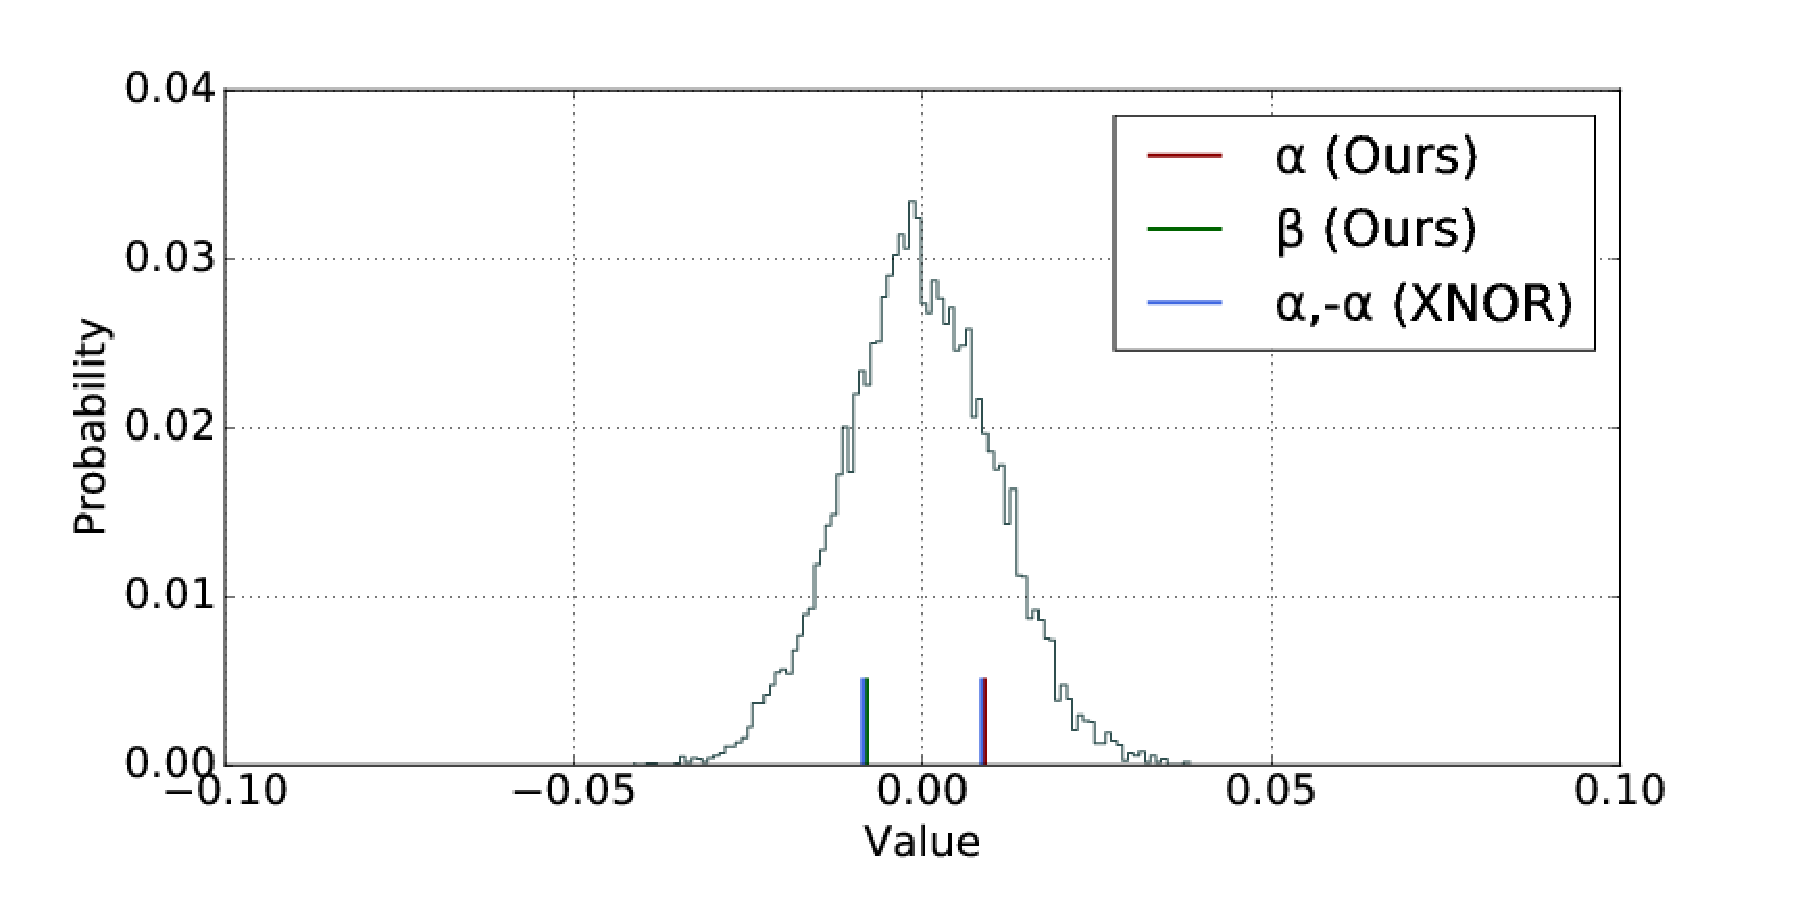
\includegraphics[page=1,width=0.5\columnwidth]{figures/figure21222324.pdf} & 
           \includegraphics[page=2,width=0.5\columnwidth]{figures/figure21222324.pdf}\\
           (1) & (2)\\
           \includegraphics[page=3,width=0.5\columnwidth]{figures/figure21222324.pdf} & \includegraphics[page=4,width=0.5\columnwidth]{figures/figure21222324.pdf}\\
           (3) & (4)\\  
\end{tabular}
\end{center}
\caption{Sub-figures (1) to (4) show the train-time variation of $\alpha$ and $\beta$ for a layer filter. Initially, $\alpha$ and $\beta$ have nearly equal magnitudes, similar to the XNOR-Net formulation, but as we progress to (4), we see that $\alpha$ and $\beta$ have widely different magnitudes.% and an approximation with only one scaling constant would be off compared to our $\alpha$-$\beta$ approximation.
Having just one scaling constant (XNOR-Net) would be a comparatively poor approximator.}
        \label{fig:alphabetaovertime}
\end{figure*}
\begin{figure*}[t]
\begin{center}
\begin{tabular}{cc}
           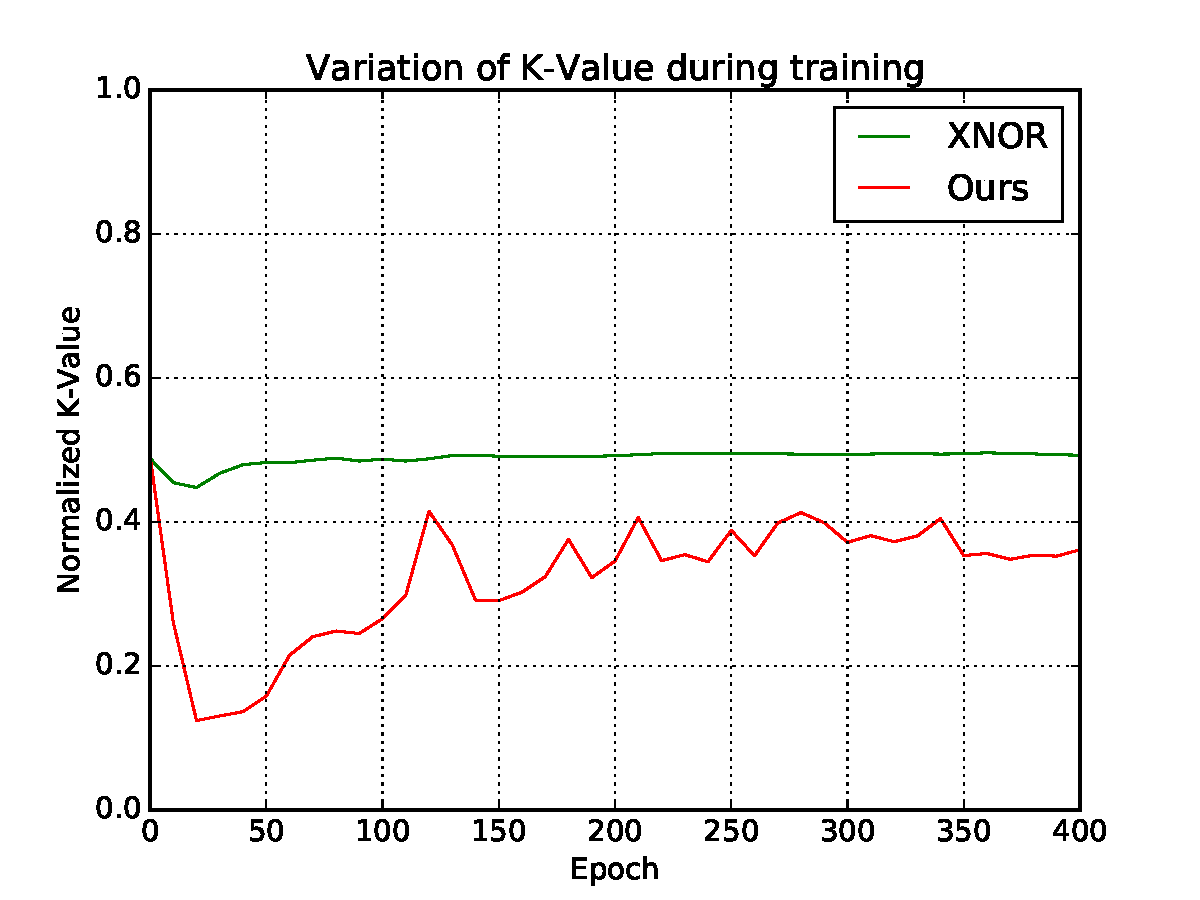
\includegraphics[width=0.5\textwidth]{figures/figure_1.pdf} & 
           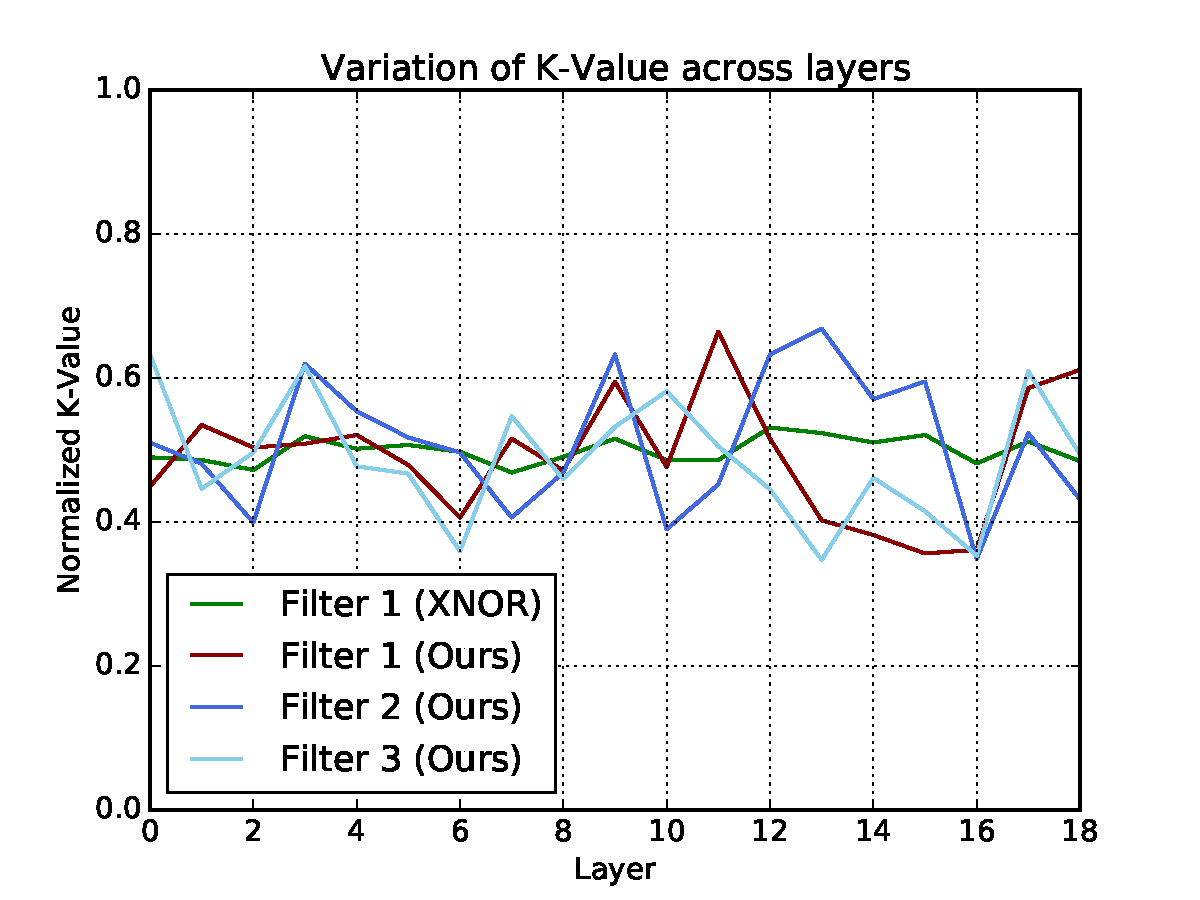
\includegraphics[width=0.5\textwidth]{figures/figure_3.pdf}\\
           (1) & (2)\\ 
\end{tabular}
\end{center}
\caption{(1) shows the variation of the normalized K-value over time during training. It falls initially but converges eventually to 0.35. The normalized K-value for XNOR-Net remains almost at 0.5 till the end. (2) shows the variation of normalized K values on random filters across layers. The K-value corresponding to DAB-Net varies across layers based on the distribution of weights of the specific layer, which is not captured by XNOR-Net.}
        \label{fig:alphabetaovertime}
\end{figure*}

\subsection{Results}

\noindent We compare the accuracies of our distribution aware binarization algorithm for WBin and FBin models on the TU-Berlin and Sketchy datasets. Note that higher accuracies are an improvement, hence stated in green in Table \ref{table:tub_recacc}. \\

\noindent On the TU-Berlin and Sketchy datasets in Table \ref{table:tub_recacc}, we observe that FBin DAB-Net models consistently perform better over their XNOR-Net counterparts. They improve upon XNOR-Net accuracies by 0.8\%, 2.5\%, and 1.5\% in Sketch-A-Net, ResNet-18, and GoogleNet respectively on the TU-Berlin dataset. Similarly, they improve by 2.0\%, 1.4\%, and 0.6\% respectively on the Sketchy dataset. We also compare them with state-of-the-art sketch classification models in Table \ref{table:sketchcomp}. We find that our compressed models perform significantly better than the original sketch models and offer compression, runtime and energy savings additionally.




\footnotetext{It is the sketch-a-net SC model trained with additional imagenet data, additional data augmentation strategies and considering an ensemble, hence would not be a direct comparison}

\noindent Our DAB-Net WBin models attain accuracies similar to BWN WBin models and do not offer major  improvements mainly because WBin models achieve FPrec accuracies already, hence do not have much scope for improvement unlike FBin models. Thus, we conclude that our DAB-Net FBin models are able to attain significant accuracy improvements over their XNOR-Net counterparts when everything apart from the binarization method is kept constant.


\subsection{XNOR-Net vs DAB-Net}

\noindent We measure how $K$, $\alpha$, and $\beta$ vary across various layers over time during training, and these variations are observed to be quite different from their corresponding values in XNOR-Net. These observations show that binarization can approximate a network much better when it is distribution-aware (like in our technique) versus when it is distribution-agnostic (like XNOR-Nets).

\subsubsection{Variation of $\alpha$ and $\beta$ across Time}

\noindent We plot the distribution of weights of a randomly selected filter belonging to a layer and observe that $\alpha$ and $\beta$ of DAB-Net start out to be similar to $\alpha$ and $-\alpha$ of XNOR-Nets, since the distributions are randomly initialized. However, as training progresses, we observe as we go from Subfigure (1) to (4) in Figure \ref{fig:alphabetaovertime}, the distribution eventually becomes non-symmetric and complex, hence our values  significantly diverge from their XNOR-Net counterparts. This divergence signifies a better approximation of the underlying distribution of weights in our method, giving additional evidence to our claim that the proposed DAB-Net technique gives a better representation of layer weights, significantly different from that of XNOR-Nets.

\subsubsection{Variation of $K$ across Time and Layers}\label{sec:kacrosslayers}

\noindent We define \textit{normalized} $K$ as the $\frac{K}{n}$ for a layer filter. For XNOR-Nets, $K$ would be the number of values below zero in a given weight filter - which has minimal variation, and does not take into consideration the distribution of weights in the filter - as $K$ in this case is simply the number of weights below a certain fixed global threshold, zero. However, we observe that the $K$ computed in DAB-Net varies significantly across epochs initially, but slowly converges to an optimal value for the specific layer as shown in Figure \ref{fig:alphabetaovertime}.\\

\noindent We also plot the variation of \textit{normalized} $K$ values for a few randomly chosen filters indexes across layers and observe that it varies across layers, trying to match the distribution of weights at each layer. Each filter has its own set of weights, accounting for the differences in variation of $K$ in each case, as shown in Figure \ref{fig:alphabetaovertime}.

\section{Summary}

\noindent We have proposed an optimal binary representation for network layer-weights that takes into account the distribution of weights, unlike previous distribution-agnostic approaches. We showed how this representation could be computed efficiently in $n.logn$ time using dynamic programming, thus enabling efficient training on larger datasets. We applied our technique on various datasets and noted significant accuracy improvements over other full-binarization approaches. 
%--------------------------------------------------------
\chapter{Hybrid Binary Networks}
\label{ch:hbn}
\noindent As Figure \ref{fig:introdiag} shows, some layers' activations are binarizable (produce lower error when binarized) while other layers give high binarization errors. In this chapter, we will explore the second question: Which layers are more important than other layers in a network?

\begin{figure}[h]
\centering
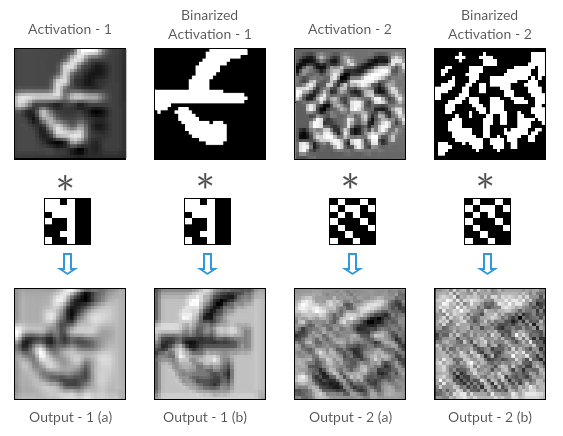
\includegraphics[width=0.8\textwidth]{figures/Intro-Diagram.png}
\caption{Convolution of binary and non-binary activations of two different layers. Note that the error introduced due to binarization is minimal in the first pair compared to the second. Hence, efficiently deciding \textit{which} layers to binarize could contribute significantly to the overall accuracy of the network and not damage the speed-ups.}
\label{fig:introdiag}
\end{figure}

\section{Hybrid Binarization}

\noindent We define certain conventions to be used throughout the paper. We define a WBin CNN to be a CNN having the weights of convolutional layers binarized (referred to as WeightBinConv layers), FBin CNN to be a CNN having both inputs and weights of convolutional layers binarized (referred to as FullBinConv layers) and FPrec CNN to be the original full-precision network having both weights and inputs of convolutional layers in full-precision (referred to as Conv layers). We compare the FBin and WBin networks with FPrec networks at specific layers.\\

\noindent Table \ref{table:versions_imagenet} and Table \ref{table:tub_recacc} in the Experiments section show test accuracies for WBin, FBin and FPrec networks of different models. Observe that there is very little loss in accuracy from FPrec to WBin networks with significant memory compression and fewer FLOPs. However, as we go from WBin to FBin networks, there is a significant drop in accuracy along with the trade-off of significantly lower FLOPs in FBin over WBin networks. Hence, we focus on improving the accuracies of FBin networks along with preserving the lower FLOPs as far as possible by investigating which activations to binarize.


\begin{figure}[t]
\centering
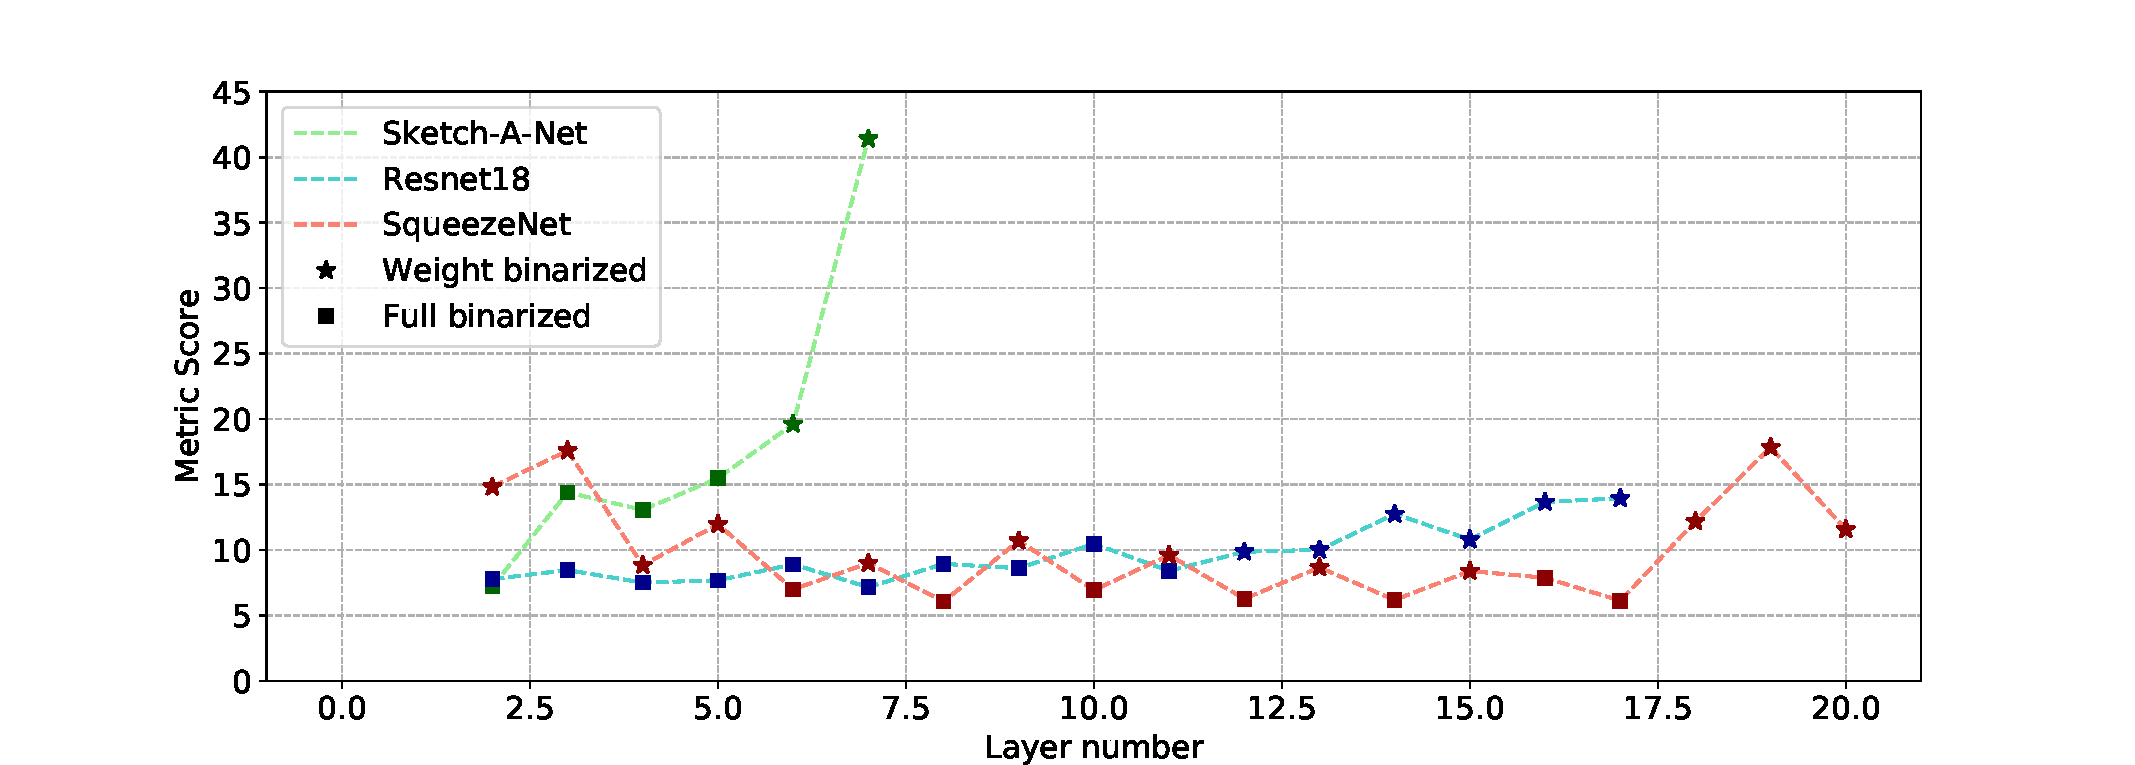
\includegraphics[width=1.0\columnwidth]{figures/metric.pdf}
\caption{Binarization-error metric across layers for Sketch-A-Net, ResNet-18, and SqueezeNet. Stars indicate that the layer was replaced with a WeightBinConv layer, while squares indicate the FullBinConv layer was retained in the FBin model. We see that the algorithm selects the last layers in the case of Sketch-A-Net and ResNet, while in the case of SqueezeNet, it selects the first four, last three and some alternate intermediate layers to be replaced by WeightBinConv layers, retaining the rest  as FullBinConv layers.}
\label{fig:metric}
\end{figure}

\subsection{Error Metric: Optimizing Speed \& Accuracy}
\noindent Full-precision inputs $\mathbf{I} \in \mathbb{R}^n$, are approximated by binary matrix $\mathbf{I_B} \in \mathbb\{-1,+1\}^n$. The optimal binary representation $\mathbf{I_B}$ is calculated by
\begin{equation}\mathbf{I_B}^\ast  = argmin(\parallel\mathbf{I}-\mathbf{I_B}\parallel^2)\end{equation}
XNOR-Net\cite{rastegari2016xnor} minimized the error function:
\begin{equation} \mathbf{E} = \frac{\parallel \mathbf{I} - \mathbf{I_B} \parallel^2}{n}\end{equation}
In order to do that, they maximized $\mathbf{I}^\top\mathbf{I_B}$ and proposed the binary activation $\mathbf{I_B}$ to be 
\begin{equation}\mathbf{I_B}^\ast = \underset{\mathbf{\mathbf{I_B}}}{\mathrm{argmax}}(\mathbf{I}^\top\mathbf{I_B}), \mathbf{I_B} \in \{-1,+1\}^n , \mathbf{I} \in \mathbb{R}^n \end{equation}, obtaining the optimal $\mathbf{I_B}^\ast$ can be shown to be  $sgn(\mathbf{I}).$\\ 

\noindent We need to investigate {\it where} to replace FullBinConv with WeightBinConv layers. In order to optimize for accuracy, we need to measure the efficacy of the binary approximation for inputs to any given layer. A good metric of this is the average error function calculated over a subset of training images $\mathbf{E}$ (defined in Eq. 2) used to calculate the optimal $I_B$ itself, which is explicitly being minimized in the process. Hence, we use that error function to capture the binarization error.\\

\noindent Similarly to optimize speed, we need to convert layers with low number of FLOPs to WeightBinConv and layers having high number of FLOPs should be kept in FullBinConv. Since we need to jointly optimize both, we propose a metric that tries to achieve a good tradeoff between the two quantities. A simple but effective metric is the linear combination \begin{equation} \mathbf{M} = \mathbf{E} + \gamma \cdot \frac{1}{\mathbf{NF}} \end{equation} where $\gamma$ is the tradeoff ratio, $\mathbf{NF}$ is the number of flops in the layer and $\mathbf{E}$ is the binarization error per neuron. The trade-off ratio $\gamma$ is a hyperparameter which ensures that both the terms are of comparable magnitude. Figure \ref{fig:metric}, captures the layer-wise variation of the error metric across multiple models.

\subsection{Partitioning Algorithm}

\noindent We aim to partition the layers of a network into two parts, one set of layers to keep FullBinConv and the other set which are replaced with WeightBinConv layers. A naive but intuitive partitioning algorithm would be to sort the list of metric errors {\bf $M$} and replace FullBinConv layers which have highest error values {\bf $M_i$} one-by-one with WeightBinConv layers, train new hybrid models and stop when the accuracies in the retrained models stop improving i.e when the maxima in accuracy v/s flops tradeoff is reached. However, we need a partitioning algorithm which gives informed guesses on where are the effective places to partition the set. This would avoid the long retraining times and large resources required to try every possible option for a hybrid model. We propose a layer selection algorithm that gives informed partitions from a trained FBin model, helping us to determine which layers are to be converted to WeightBinConv and which layers are to be converted to FullBinConv without having to train all possible hybrid models from scratch.\\

\begin{algorithm}[t]
\centering
\caption{{\bf Partition Algorithm} \\Marks layers for binarization and creates a hybrid network.}
\begin{algorithmic}[1]
\State Inputs $\Rightarrow$Layer-wise Binarization Errors
\\

\State \texttt{Initialization}
\State $P$ = Total convolutional layers
\State $R$ = Hybridization Ratio
\State ToConvert = List() \\
\State \texttt{Mark binary layers}
\For{$N$ = 2 to P}
	\State Compute KMeans with $N$ means
	\State $K$ = Number of layers in highest-error cluster
	\If{$K/P \leq R$}
	\For{$Q$ in high-error clusters}
        	\State ToConvert.add($Q$) \Comment{Add layer $Q$ }
    \EndFor
    \State Break
	\EndIf
\EndFor 

\\

\State \texttt{Create Hybrid Network}
\State HybridNet = ()

\State HybridNet.Add(Conv)
\\
\For{$N$ = 2 to P}
        \If{$N$ in ToConvert}
            \State HybridNet.Add(WeightBinConv)
        \Else
        	\State HybridNet.Add(FullBinConv)
        \EndIf
\EndFor
\\
\State Output $\Rightarrow$ HybridNet

\end{algorithmic}
\label{alg:partitionalgo}
%\vspace*{-0.75cm}
\end{algorithm}
\begin{figure}[t]
\centering
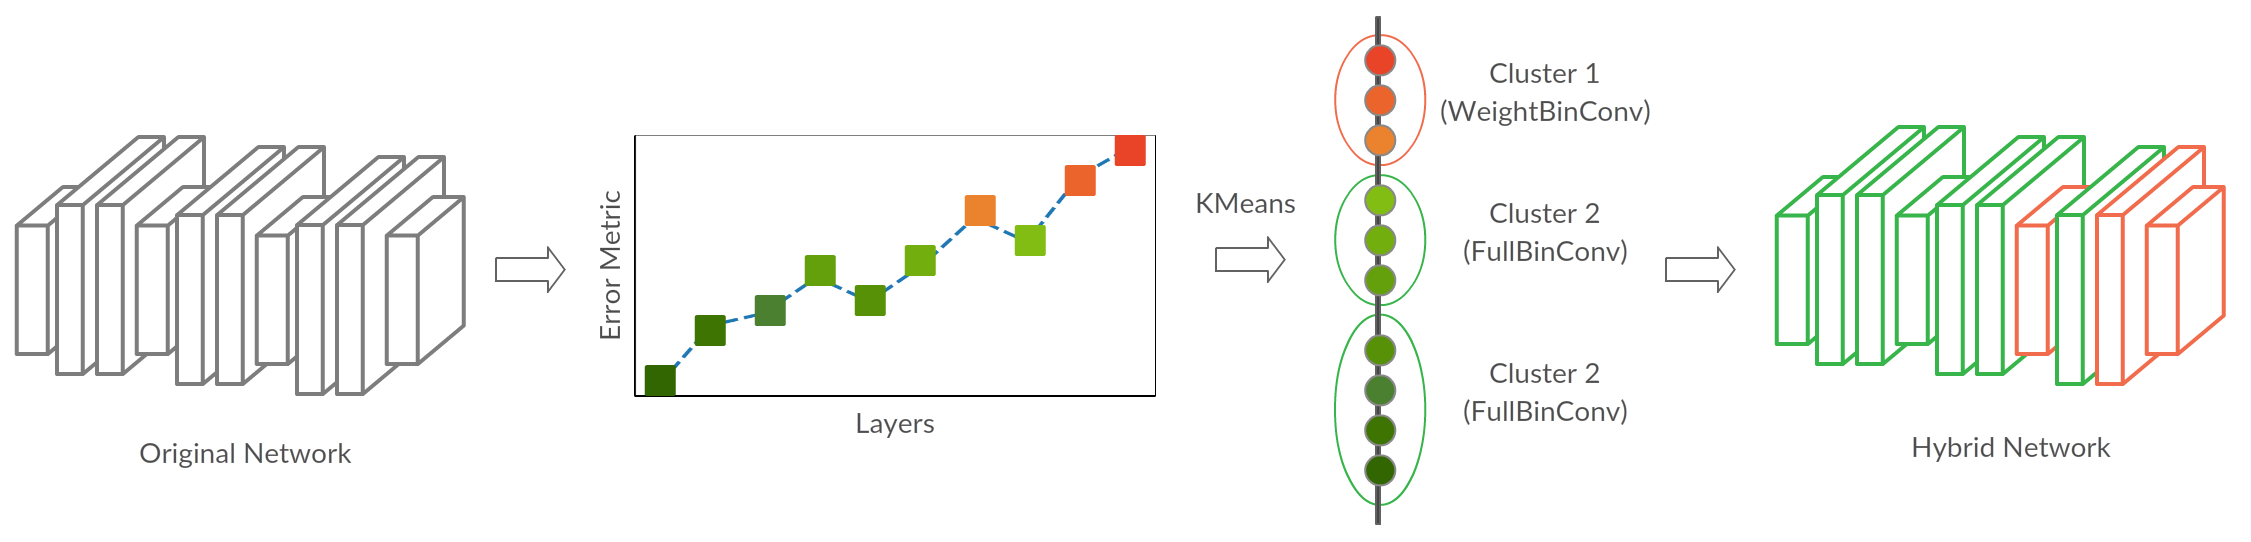
\includegraphics[width=1.0\textwidth]{figures/Main-Algo-Diagram.png}
\caption{The Procedure: Error metrics from binarization of inputs to the network layers are partitioned into clusters using K-means. The highest error cluster indicates the inputs that are not binarized to generate the hybrid version.}
\label{fig:pipeline}
%\vspace{-1.5cm}
\end{figure}
\noindent Our algorithm starts by taking a trained FBin model. We pass in a subset of the training images and calculate the average error metric for all layers over them. Then we perform K-Means Clustering on the metric values with each point being the metric error of layers as shown in Figure \ref{fig:metric}. We perform the K-Means Clustering for different values of the number of clusters. We find a suitable number of clusters such that the ratio of layers in the highest-error cluster ($K$) to the total number of convolutional layers ($P$) is less than a hyperparameter, which we define as the Hybridization Ratio $R$. Layers with terms falling in the highest mean cluster are converted to WeightBinConv, while the ones in all other clusters are left as FullBinConv. A flow of the algorithm is illustrated in Figure \ref{fig:pipeline} and is explained step-by-step in Algorithm \ref{alg:partitionalgo}. We show metric scores of various layers for different networks in Figure \ref{fig:metric} and indicate which layers are replaced with WeightBinConv/FullBinConv layers. This algorithm guides in forming the architecture of the hybrid model, which is then trained from scratch obtaining the accuracies given in the tables presented in the Experiment section. Note that this algorithm does not change the configuration of the model; it only converts certain layers to their binarized versions.\\

\noindent To give an intuition of what the Hybridization ratio $R$ means, a low $R$ would indicate we need the number of WeightBinConv layers to be low, ensuring a high asymmetry between errors in WeightBinConv and FullBinConv layers, prioritizing saving computational cost. Conversely, a higher $R$ would prioritize accuracy over computational cost. $R$ was set to be 0.4 for AlexNet and ResNet-18, and 0.6 for Squeezenet. Variation with different values of $R$ is further discussed in the experiments section.

\subsection{Impact on Speed and Energy Use}
\noindent {\bf Computational Speedups}: Convolutional operations are computationally expensive. For each convolution operation between an image $\mathbf{I} \in \mathbb{R}^{c_{in} \times h_I \times w_I}$ and weight $\mathbf{W} \in \mathbb{R}^{c_{out} \times h \times w}$, the number of MAC operations required $N$ are $\approx C_{in}C_{out}N_WN_I$ where $N_W = wh$ and $N_I = w_Ih_I$. According to benchmarks done in XNOR-Net, the current speedup obtained in these operations is 58x after including the overhead induced by computing $\alpha$. Accordingly, in later sections, we take one FLOP through a layer as equivalent to 58 binary operations when weights and inputs are binarized. \\ 

\noindent {\bf Exploiting filter repetitions}: The number of unique convolutional binary filters is bounded by the size of the filter \cite{courbariaux2016binarized}. As most of our intermediate convolutional layers have $3\times3$ filters which only have $2^9$ unique filters, we find that the percentage of unique filters decreases as we go deeper into the network. We can exploit this fact to simply prune filters and use that in calculating speedups for binary networks. More details regarding how the speedup was computed is included in the supplementary material.

%------------------------------------------------------------------------
\section{Experiments and Results}

\noindent We report and compare accuracies, speedups and compression between the FPrec model, different kinds of binarization models (WBin and FBin), and their generated hybrid versions of the same. We also present a detailed comparison of our method with several different compression techniques applied on AlexNet \cite{alex2012alexnet}, ResNet-18 \cite{he2016deep}, Sketch-A-Net \cite{eitz2012hdhso} and SqueezeNet \cite{iandola2016squeezenet}. \\

\noindent We empirically demonstrate the effectiveness of hybrid binarization on several benchmark image and sketch datasets. We show that our approach is robust and can generalize to different types of CNN architectures across domains.

\subsection{Datasets and Models}
\noindent Binary Networks have achieved accuracies comparable to full-precision networks on limited domain/simplified datasets like CIFAR-10, MNIST, SVHN, but show drastic accuracy losses on larger-scale datasets. To compare with state-of-the-art vision, we evaluate our method on ImageNet\cite{deng2009imagenet}. To show the robustness of our approach, we test it on sketch datasets, where models fine-tuned with ImageNet are demonstrably not suitable as shown in\cite{yu2015sketch}. Binary networks might be better suited for sketch data due to its binary nature and sparsity of information in the data. \\

\noindent {\bf ImageNet:} The benchmark dataset for evaluating image recognition tasks, with over a million training images and 50,000 validation images. We report the single-center-crop validation errors of the final models.\\

\noindent {\bf TU-Berlin:} The TU-Berlin \cite{eitz2012hdhso} sketch dataset is the most popular large-scale free-hand sketch dataset containing sketches of 250 categories, with a human sketch-recognition accuracy of 73.1\% on average.\\ 

\noindent {\bf Sketchy:} It is a recent large-scale free-hand sketch dataset containing 75,471 hand-drawn sketches from across 125 categories. This dataset was primarily used to cross-validate results obtained on the TU-Berlin dataset and ensure that our approach is robust to the variation in collection of data.\\

\begin{table}[t]
\centering
\begin{tabular}{|l|c|c|c|c|l|}
\hline
{\bf Technique} & {\bf Acc-Top1} & {\bf Acc-Top5} & {\bf W/I} & {\bf Mem} & {\bf FLOPs} \\
\hline
\multicolumn{6}{|c|}{\sc { \bf AlexNet}} \\
\hline
BNN & 39.5\% & 63.6\% & 1/1 & 32x & 121 (1x)\\
XNOR & 43.3\% & 68.4\% & 1/1 & 10.4x & {\bf 121 (1x)} \\
Hybrid-1 & 48.6\% & 72.1\% & 1/1 & 10.4x & 174 (1.4x)\\
Hybrid-2 & {\bf 48.2\%} & {\bf 71.9\%} & 1/1 & {\bf 31.6x} & 174 (1.4x)\\
\hline
HTCBN & 46.6\% & 71.1\% & 1/2 & 31.6x & 780 (6.4x)\\
DoReFa-Net & 47.7\% & - & 1/2 & 10.4x & 780 (6.4x)\\
\hline
\multicolumn{6}{|c|}{\sc { \bf Res-Net 18}} \\
\hline
BNN & 42.1\% & 67.1\% & 1/1 & 32x & 134 (1x)\\
XNOR & 51.2\% & 73.2\% & 1/1 & 13.4x & {\bf 134 (1x)} \\
Hybrid-1 & 54.9\% & 77.9\% & 1/1 & 13.4x & 359 (2.7x)\\
Hybrid-2 & {\bf 54.8\%} & {\bf 77.7\%} & 1/1 & {\bf 31.2x} & 359 (2.7x)\\
\hline
HTCBN & 53.6\% & - & 1/2 & 31.2x & 1030 (7.7x)\\
\hline
\end{tabular}
\caption{
A detailed comparison of accuracy, memory use, FLOPs with popular benchmark compression techniques on ImageNet. Our hybrid models outperform other 1-bit activation models and perform on par with 2-bit models while having a significantly higher speedup. Hybrid-2 models have the last layer binarized.}
\label{table:imagenet_fullcomp}
\end{table}

\noindent We use the standard splits with commonly used hyper-parameters to train our models. Each FullBinConv block was structured as in XNOR-Net (Batchnorm-Activ-Conv-ReLU). Each WeightBinConv and Conv block has the standard convolutional block structure (Conv-Batchnorm-ReLU). Weights of all layers except the first were binarized throughout our experiments unless specified otherwise. Note that FLOPs are stated in millions in all diagrams and sections. All networks are trained from scratch independently. The architecture of the hybrid network once designed does not change during training. Additional details about the datasets, model selection and layer-wise description of each of the hybrid models along with experimental details can be found in the supplementary material. 

\subsection{Results}

\noindent We compare FBin, WBin, Hybrid and FPrec recognition accuracies across models on ImageNet, TU-Berlin and Sketchy datasets. Note that higher accuracies are an improvement, hence stated in green in the table, while higher FLOPs mean more computational expense, hence are stated in red. W/I indicates the number of bits used for weights and inputs to the layer respectively. Note that in the table, the compression obtained is only due to the weight binarization, while the decrease in effective FLOPs are due to activation binarization.\\

\noindent On the ImageNet dataset in Table \ref{table:versions_imagenet}, hybrid versions of AlexNet and ResNet-18 models outperform their FBin counterparts in top-1 accuracy by 4.1\% and 3.6\% respectively, and around 20x compression for both. We also compare with the results of other compression techniques in Table \ref{table:imagenet_fullcomp}.\\

\begin{table}[t]
\centering
\begin{tabular}{|l|c|c|c|c|l|}
\hline
\multirow{2}{*}{\bf Model} & \multirow{2}{*}{\bf Method} & \multicolumn{2}{c|}{\sc { \bf Accuracy}} & \multirow{2}{*}{\bf Mem} & \multirow{2}{*}{\bf FLOPs}\\
\cline{3-4}
 &  & Top-1 & Top-5 &   &  \\
\hline
\multirow{5}{*}{AlexNet} & FPrec & 57.1\% & 80.2\% & 1x & 1135 (9.4x)\\
 & WBin (BWN) & 56.8\% & 79.4\% & 10.4x & 780 (6.4x)\\
 & FBin (XNOR) & 43.3\% & 68.4\% & 10.4x & {\bf 121 (1x)} \\
 & Hybrid-1 &  48.6\% & 72.1\% & 10.4x & 174 (1.4x)\\
 & Hybrid-2 & {\bf  48.2\%} & {\bf 71.9\%} & {\bf 31.6x} & 174 (1.4x)\\
\hline
Increase & Hybrid vs FBin & +4.9\% & +3.5\% & +21.2x & +53 (+0.4x) \\
\hline
\multirow{5}{*}{ResNet-18} & FPrec & 69.3\% & 89.2\% & 1x & 1814 (13.5x)\\
 & WBin (BWN) & 60.8\% & 83.0\% & 13.4x & 1030 (7.7x)\\
 & FBin (XNOR) & 51.2\% & 73.2\% & 13.4x & {\bf 134 (1x)}\\
 & Hybrid-1 & 54.9\% & 77.9\% & 13.4x & 359 (2.7x)\\
 & Hybrid-2 & {\bf 54.8\%} & {\bf 77.7\%} & {\bf 31.2x} & 359 (2.7x)\\
\hline
Increase & Hybrid vs FBin & +3.6\% & +4.5\% & +17.8x & +225 (+1.7x)\\
\hline
\end{tabular}
\caption{Our hybrid models compared to FBin, WBin and NoBin models on Imagenet in terms of accuracy, memory and computations expense.}
\label{table:versions_imagenet}
\end{table}

\begin{table}[t]
\centering
\begin{tabular}{|l|c|c|c|c|l|}
\hline
\multirow{2}{*}{\bf Model} & \multirow{2}{*}{\bf Method} & \multicolumn{2}{c|}{\sc { \bf Accuracy}} & \multirow{2}{*}{\bf Mem} & \multirow{2}{*}{\bf FLOPs}\\
\cline{3-4}
 &  & TU-Berlin & Sketchy &  &  \\
\hline
\multirow{4}{*}{Sketch-A-Net} & FPrec & 72.9\% & 85.9\% & 1x & 608 (7.8x)\\
 & WBin (BWN) & 73\% & 85.6\% & 29.2x & 406 (5.2x)\\
% & FBin (XNOR) & 48.2\% & 38.6\% & 29.2x & 78 (1x) \\
 & FBin (XNOR) & 59.6\% & 68.6\% & 19.7x & {\bf 78 (1x)} \\
 & Hybrid & {\bf 73.1\%} & {\bf 83.6\%} & {\bf 29.2x} & {\bf 85 (1.1x)}\\
\hline
Increase & Hybrid vs FBin & +13.5\% & +15.0\% & +9.5x & +7 (+0.1x)\\
\hline
\multirow{4}{*}{ResNet-18} & FPrec & 74.1\% & 88.7\% & 1x & 1814 (13.5x) \\
 & WBin (BWN) & 73.4\% & 89.3\% & 31.2x & 1030 (7.7x)\\
 & FBin (XNOR) & 68.8\% & 82.8\% & 31.2x & {\bf 134 (1x)} \\
 & Hybrid  & {\bf 73.8\%} & {\bf 87.9\%} & {\bf 31.2x} & 359 (2.7x)\\
\hline
Increase & Hybrid vs FBin & +5.0\% & +5.1\% & - & +225 (+1.7x)\\
\hline
\end{tabular}
\caption{Our hybrid models compared to FBin, WBin and full prec models on TU-Berlin and Sketchy datasets in terms of accuracy, memory and speed tradeoff.} 
\label{table:tub_recacc}
\end{table}

\noindent On the TU-Berlin and Sketchy datasets in Table \ref{table:tub_recacc}, we find that Sketch-A-Net and ResNet-18 have significantly higher accuracies in the hybrid models compared to their FBin counterparts, a 13.5\% gain for Sketch-A-Net and 5.0\% for ResNet-18. \\

\noindent These hybrid models also achieve over 29x compression over FPrec models and with a reasonable increase in the number of FLOPs - a mere 7M increase in Sketch-A-Net and a decent 225M increase in ResNet-18. We also compare them with state-of-the-art sketch classification models in Table \ref{table:sketchcomp}. Our hybrid Sketch-A-Net and ResNet-18 models achieve similar accuracies to state-of-the-art, while also highly compressing the models upto 233x compared to the AlexNet FPrec model. \\

\begin{figure*}
\centering
\begin{tabular}{cc}
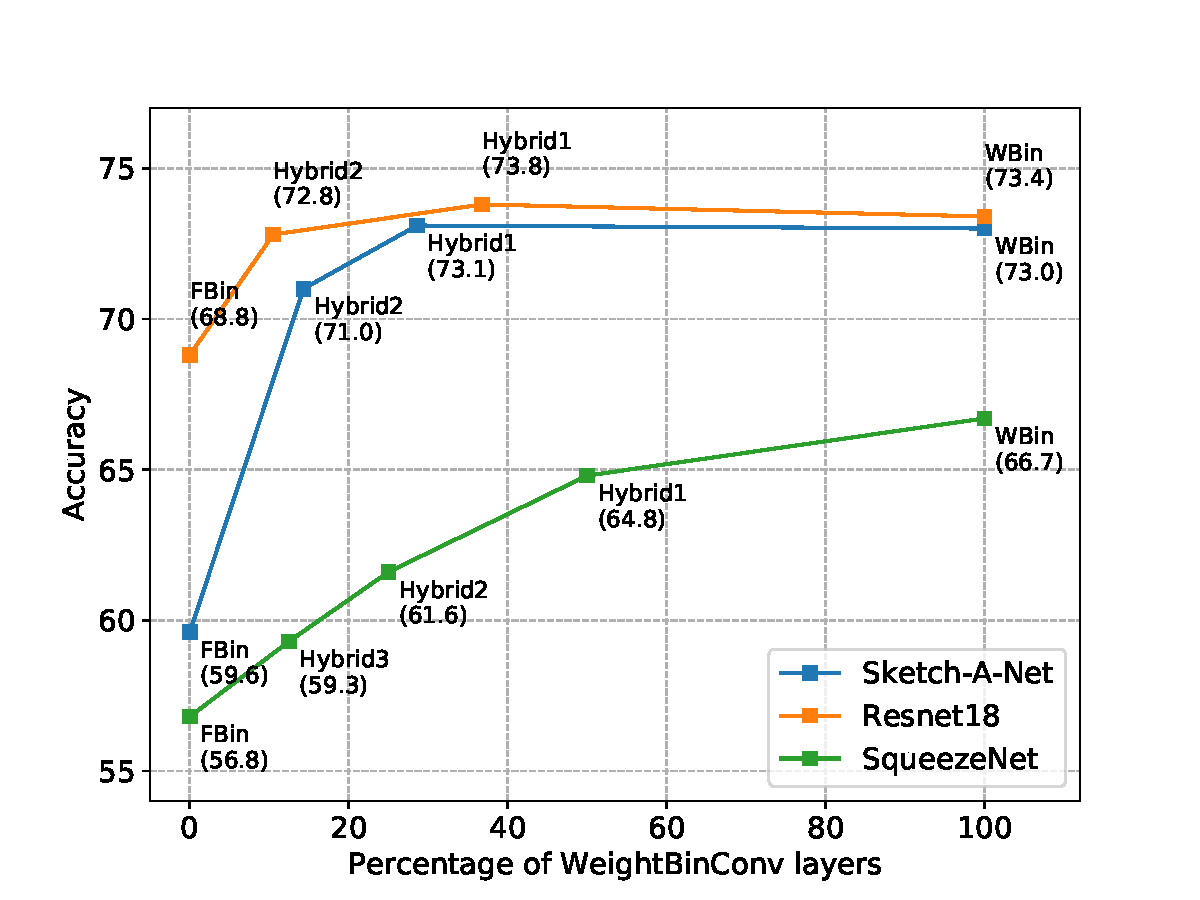
\includegraphics[width=0.5\textwidth]{figures/Figure_1.pdf} &
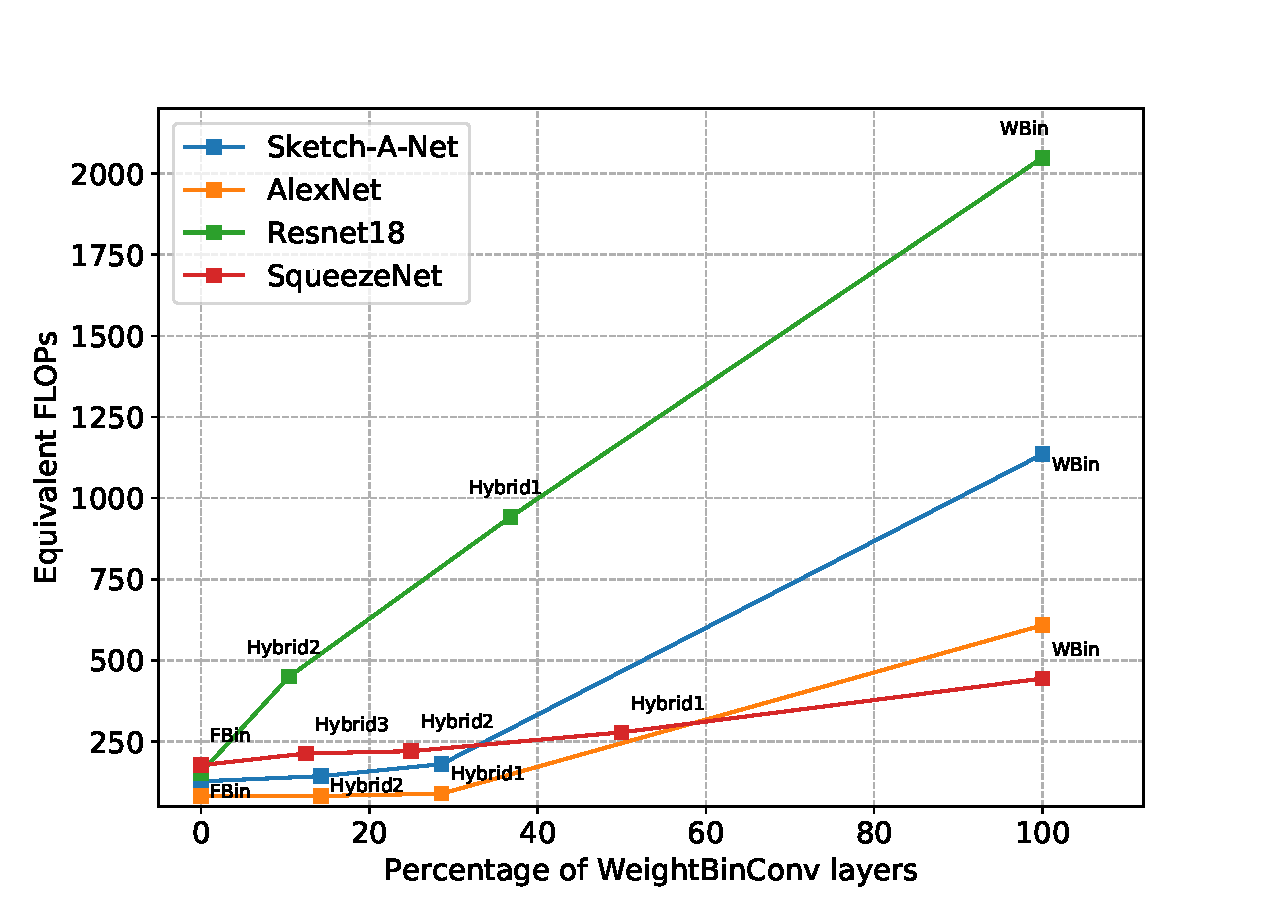
\includegraphics[width=0.5\textwidth]{figures/Figure_2.pdf}\\
\end{tabular}
\caption{Trade-off between WeightBinConv layers and accuracy on the TU-Berlin dataset is shown in the left figure, while the trade-off between weight binarized layers and speedup is shown in the right figure. Early on, we observe that a small increase in the percentage of WeightBinConv layers leads to a large increase in accuracy and a marginal decrease in speed. We achieve accuracies comparable to the WBin model with much fewer WeightBinConv layers.
}
\label{fig:tradeoff}
\end{figure*}

Thus, we find that our hybrid binarization technique finds a balance between sacrificing accuracy and gaining speedups and compression for various models on various datasets.
\begin{table}[t]
\begin{center}
\begin{tabular}{|l|c|c|c|l|}
\hline
{\bf Model} & {\bf Acc} & {\bf Mem} & {\bf FLOPs}\\
\hline
AlexNet-SVM & 67.1\% & 1x & 1135 (13.4x)\\
AlexNet-Sketch & 68.6\% & 1x & 1135 (13.4x)\\
Sketch-A-Net SC & 72.2\% & 8x & 608 (7.2x)\\
\hline
Sketch-A-Net-Hybrid & {\bf 73.1\%} & {\bf 233x} & {\bf 85 (1x)}\\
ResNet18-Hybrid & {\bf 73.8\%} & - & {\bf 359 }\\
\hline
Humans & {73.1\%} & - & - \\
Sketch-A-Net-2  \footnotemark \cite{yu2017sketch} & {\bf 77.0\%} & 8x & 608 (7.2x)\\
\hline
\end{tabular}
\footnotetext{It is the sketch-a-net SC model trained with additional imagenet data, additional data augmentation strategies and considering an ensemble, hence would not be a direct comparison}
\end{center}
\caption{A comparison between state-of-the-art single model accuracies of recognition systems on the TU-Berlin dataset.}
\label{table:sketchcomp}
\end{table}

\subsection{Algorithmic Insights}
\noindent We gained some insights into where to binarize from our investigation. We provide them as a set of practical guidelines to enable rapid prototyping of hybrid models, which gives meaningful insights into which layers were partitioned.\\

\noindent {\bf Convert layers towards the end to WeightBinConv:} It is observed that later layers typically have high error rates, more filter repetitions, and lower computational cost. Hence, the algorithm tends to start converting models to Hybrid from the last layers. \\

\noindent {\bf Convert the smaller of the layer placed parallely to WeightBinConv:} It is a good idea to convert the smaller of the parallely placed layers in the architecture like Residual layers in the ResNet architecture to WeightBinConv, since converting them to WeightBinConv would not damage the computational speedup obtained by the parallel FullBinConv layers.\\

\noindent {\bf Pick a low Hybridization Ratio:} Try to pick low values of the Hybridization Ratio $R$, ensuring a low proportion of number of layers the highest-error cluster.\\

\noindent {\bf Relax the Hybridization Ratio for compact models:} Having a higher Hybridization Ratio for compact models which inherently have fewer flops leaves more layer inputs un-binarized and retains accuracy. 

\subsection{Why are layer-wise errors independent?}
\noindent Can binarization noise introduced in a layer propagate further into the network and influence other layers? Courbariaux \etal \cite{courbariaux2016binarized} provide some insights for the same. Let $\mathbf{W}$ be the weight and $\mathbf{I}$ be the input to the convolutional layer. The output of the convolution between the binary weights and inputs can be represented by \begin{equation}\mathbf{O_B} = \alpha \cdot (sgn(\mathbf{W}^\intercal) \odot sgn(\mathbf{I}))\end{equation} The desired output $\mathbf{O}$ is modelled by $\mathbf{O_B}$ along with the binarization noise $\mathbf{N}$ introduced due to the function $sgn(.)$. \begin{equation}\mathbf{O} = \mathbf{W} * \mathbf{I} = \sum_{i}^{} \mathbf{O_B}_i + \mathbf{N_i}\end{equation} When the layer is wide, we expect the deterministic term $\mathbf{O_B}$ to dominate, because the noise term $\mathbf{N}$ is a summation over many independent binarizations from all the neurons in the layer. Thus, we argue that the binarization noise $\mathbf{N}$ should have minimal propagation and do little to influence the further inputs. Hence, it is a reasonable approximation to consider the error across each layer independently of the other layers.

\subsection{Variation with the Hybridization Ratio ($R$)}
\noindent To observe the trade-off between accuracy and speedup on different degrees of binarization, we chose different values of the Hybridization Ratio ($R$) to create multiple hybrid versions of the AlexNet, ResNet-18 and SqueezeNet models. Picking a larger $R$ would result in a higher number of WeightBinConv layers. We compare these hybrid networks to their corresponding FBin and WBin versions. \\

\noindent In Figure \ref{fig:tradeoff}, we show model accuracies of AlexNet, ResNet-18 and SqueezeNet on the ImageNet dataset plotted against the number of WeightBinConv layers, starting from only FBin versions on the left, to only WBin versions on the right. We observe that in the case of AlexNet and ResNet-18, which are large models, we recover WBin accuracies quickly, at around the 35\% mark (Roughly a third of the network containing WeightBinConv layers), with low computational trade-off. We also observe that on sketch data, hybrid models tend to perform significantly better and perform on par with their WBin counterparts.\\ 

\noindent We also notice that the smaller a model, the more trade-off must be made to achieve WBin accuracy, i.e a larger Hybridization Ratio must be used. AlexNet, the largest model crosses WBin accuracy at around 32\%, while ResNet-18, being smaller, saturates at around 40\%. SqueezeNet, a much more compact model, reaches its WBin accuracy at 60\%.

\subsection{Optimizing Memory}
\noindent We measured accuracies for FBin and Hybrid variants of Sketch-A-Net and ResNet-18 models on TU-Berlin and Sketchy Datasets with weights of the last layer binarized as well as non-binarized and the results are presented in Table \ref{table:otherresults}. For AlexNet-styled architectures (Sketch-A-Net), we observe a drastic drop in accuracies (From 59.1\% to 48.3\%) on binarizing the last layer, similar to observations made in previous binarization works \cite{zhou2016dorefa,tang2017train}. \\

\begin{table}[t]
  \centering
\begin{tabular}{|l|c|c|c|c|c|}

\hline
{\bf Model} & {\bf BinType} & {\bf Last Bin?} & {\bf Acc } & {\bf Mem}\\
\hline
\multirow{2}{*}{Sketch-A-Net} & \multirow{2}{*}{FBin (XNOR)} & No & 59.6\% & 19.7x \\
 &  & Yes & 48.3\% & {\bf 29.2x} \\

\hline
\multirow{2}{*}{Sketch-A-Net} & \multirow{2}{*}{Hybrid} & No & 73.1\% & 19.7x \\
 &  & Yes & 72.0\% & {\bf 29.2x} \\
\hline
\multirow{2}{*}{Resnet-18} & \multirow{2}{*}{FBin (XNOR)} & No & 69.9\% & 13.4x \\
 &  & Yes & 68.8\% & {\bf 31.2x} \\

\hline
\multirow{2}{*}{Resnet-18} & \multirow{2}{*}{Hybrid} & No & 73.9\% & 13.4x \\
 &  & Yes & 73.8\% & {\bf 31.2x} \\
\hline
\end{tabular}
\caption{Effects of last layer weight-binarization on TU-Berlin dataset, for Sketch-A-Net and ResNet-1. Observe that our hybrid models do not face drastic accuracy drop when the last layer is weight-binarized.}
\label{table:otherresults}
\end{table}

\noindent Many efforts were made to quantize the last layer and avoid this drop. DoReFaNet and XNOR-Net did not binarize the last layer choosing to incur a degradation in model compression instead while \cite{tang2017train} proposed an additional scale layer to mitigate this effect. However, our hybrid versions are able to achieve similar accuracies (a 1\% drop for hybrid Sketch-A-Net and no drop for ResNet-18 or AlexNet) since the last layer is weight binarized instead. Hence, our method preserves the overall speedup even though we only weight-binarize the last layer, owing to the comparatively smaller number of computations that occur in this layer.\\

\noindent Note that the first layer is always a full-precision Conv layer. The reasons behind this are the insights obtained from \cite{anderson2017high}. They state that the first layer of the network functions are fundamentally different than the computations being done in the rest of the network because the high variance principal components are not randomly oriented relative to the binarization. Also, since it contains fewer parameters and low computational cost, it does not affect our experiments.

\subsection{Compressing Compact Models}
\noindent Whether compact models can be compressed further, or {\it need} all of the representational power afforded through dense floating-point values is an open question asked originally by \cite{iandola2016squeezenet}. \\

\noindent We show that our hybrid-binarization technique can work in tandem with other compression techniques, which do not involve quantization of weights/activations and that hybrid binarization is possible even on compact models. We apply hybrid binarization to SqueezeNet\cite{iandola2016squeezenet} a recent model that employed various architectural design strategies to achieve compactness. SqueezeNet achieves an 8x compression on the compact architecture of Sketch-A-Net. On applying hybrid binarization we achieve a further 32x compression, an overall 256x compression with merely 6\% decrease in accuracy. This is due to the high rate of compression inherent and further compression is difficult due to the small number of parameters. After showing that efficacy of hybrid binarization in the previous section, we show that hybrid binarization can work in combination with other compression techniques here.\\

\begin{table}[t]
\centering

\begin{tabular}{|l|c|c|c|c|l|}
 \hline
\multirow{2}{*}{\bf Model} & \multirow{2}{*}{\bf Method} & \multicolumn{2}{c|}{\sc { \bf Accuracy}} & \multirow{2}{*}{\bf Mem} & \multirow{2}{*}{\bf FLOPs}\\
\cline{3-4}
 &   & TU-Berlin & Sketchy &   &  \\
\hline
Sketch-A-Net & FPrec & 72.9\% & 85.9\% & 1x & 1135 (12.3x)\\
Squeezenet & FPrec & 71.2\% & 86.5\% & 8x & 610 (6.6x)\\
Squeezenet & WBin & 66.7\% & 81.1\% & 23.7x & 412 (4.5x)\\
\hline
Squeezenet & FBin & 56.8\% & 66.0\% & 23.7x & {\bf 92 (1x)} \\
Squeezenet & Hybrid & {\bf 64.8\%} & {\bf 79.6\%} & {\bf 23.7x} & 164 (1.8x)\\
\hline
Improvement & Hybrid vs FBin & +8.0\% & +13.6\% & - & +72 (+0.8x)\\
\hline
\end{tabular}
\caption{Our performance on SqueezeNet, an explicitly compressed model architecture. Although SqueezeNet is an inherently compressed model, our method still achieves further compression on it.}
\label{table:squeezenet}
\end{table}

\noindent Results for SqueezeNet are shown in Table \ref{table:squeezenet} for the TU-Berlin and Sketchy datasets, and we see that accuracy is only slightly lower compared to the hybridized versions of ResNet-18 and Sketch-A-Net on the same. Hybrid SqueezeNet achieves a total compression of 256x. Similarly, this technique can be combined with many techniques such as HWGQ-Net \cite{cai2017deep} which proposes an alternative layer to ReLU and repeated binarization as illustrated in \cite{tang2017train} among others. Since our primary goal is to investigate the viability of hybrid binarization, these investigations- albeit interesting, are out of the scope of our current work.

%------------------------------------------------------------------------
\section{Summary}
\noindent We proposed a novel algorithm for selective binarization of CNNs, which strikes a balance between performance, memory-savings and accuracy. The accuracies of our hybrid models were on par with their corresponding full-precision networks on TU-Berlin and Sketchy datasets, while providing the benefits of network binarization in terms of speedups, compression and energy efficiency. We successfully weight-binarized the last layers without significant accuracy drops, a problem faced by previous works in this area. We also showed that we can successfully combine the advantages of our approach with other architectural compression strategies, to obtain highly efficient models with negligible accuracy penalties. 
%--------------------------------------------------------
\chapter{Deep Expander Networks}
\label{ch:den}
\noindent How do we prune before training? In this chapter, we explore an principled way of pruning on a layer-level before training by imposing some necessary constraints on the architecture.
\begin{figure}[h]
\centering
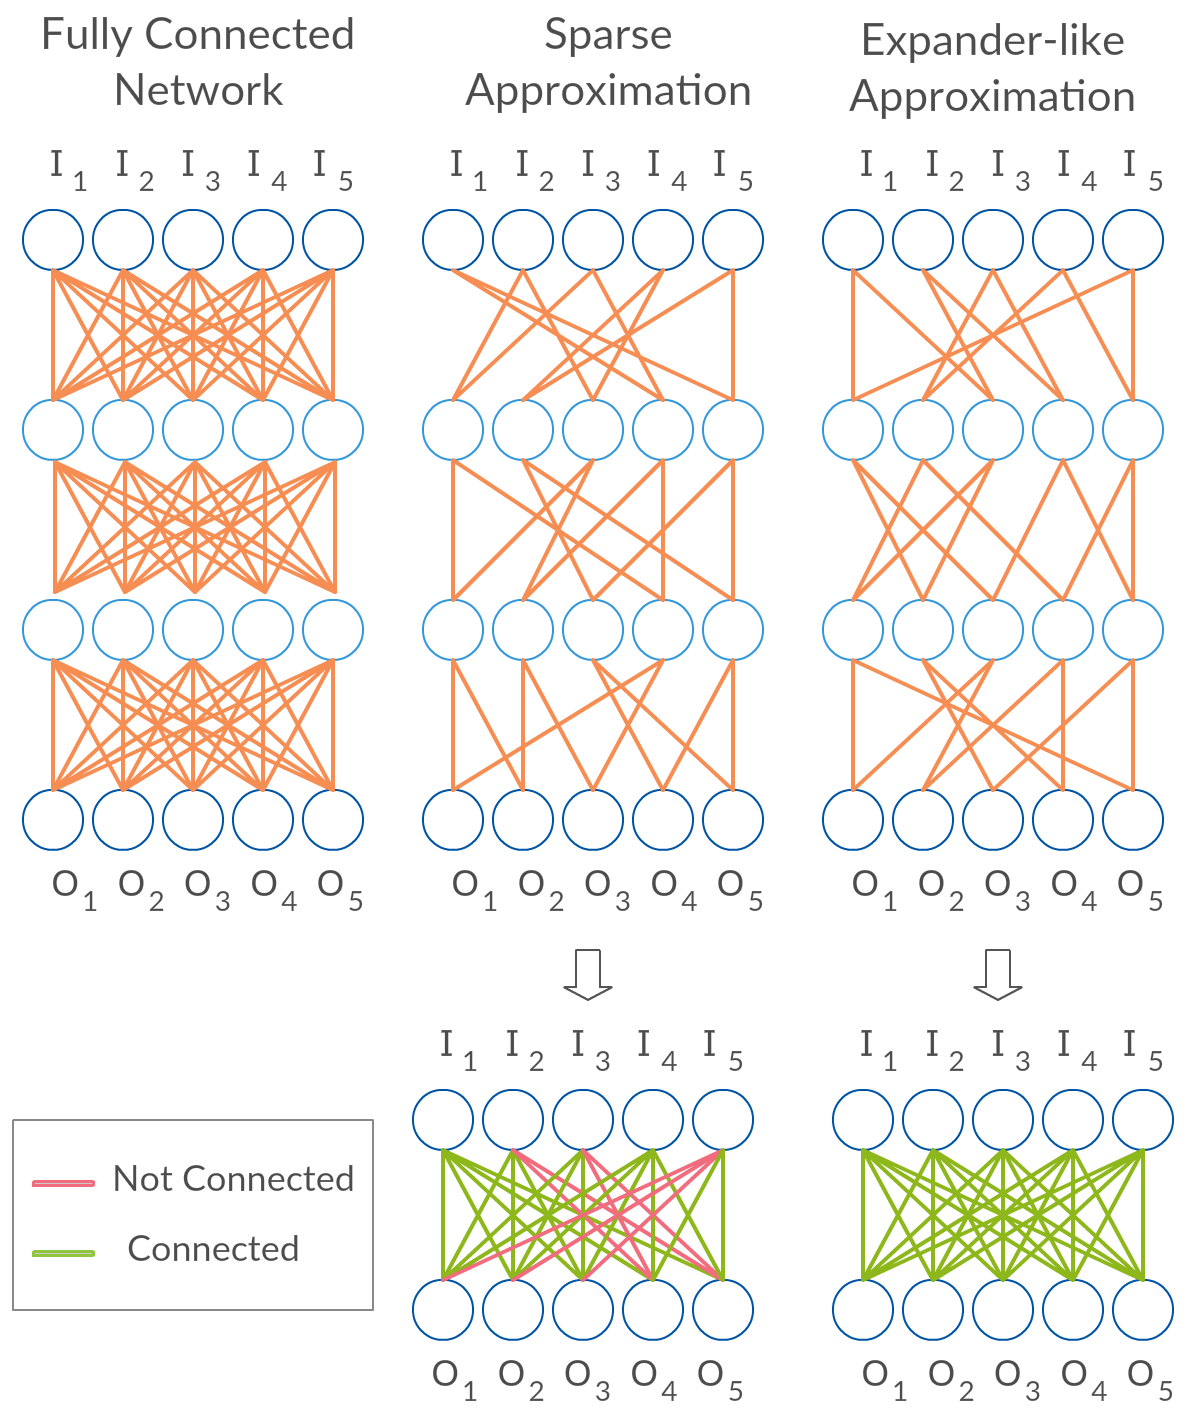
\includegraphics[width=0.4\textwidth]{figures/Expander2.png}
\caption{Popular sparse approximations are agnostic to the global information flow in a network, possibly creating disconnected components. In contrast, expander graph-based models produce sparse yet highly connected networks.}
\label{fig:intro}
\end{figure}

\section{Approach}\label{sec:approach}
\noindent Recent breakthroughs in CNN architectures like ResNet\cite{he2016deep} and DenseNet-BC\cite{huang2017densely} are ideas  based on increasing connectivity, which resulted in better performance trade-offs. These works suggest that connectivity is an important property for improving the performance of deep CNNs. In that vein, we investigate ways of preserving connectivity between neurons while significantly sparsifying the connections between them, shown in \ref{fig:intro}. Such networks are expected to preserve accuracy (due to connectivity) while being runtime efficient (due to the sparsity). We empirically demonstrate this in the later sections.

\subsection{Graphs and Deep CNNs}

\noindent We model the connections between neurons as graphs. This enables us to leverage well-studied concepts from Graph Theory like Expander Graphs. Now, we proceed to formally describe the connection between graphs and Deep CNNs.\\ 

\noindent {\bf Linear Layer defined by a Graph:} Given a bipartite graph $G$ with vertices $U, V$, the Linear layer defined by $G$, is a layer with $|U|$ input neurons, $|V|$ output neurons and each output neuron $v \in V$ is only connected to the neighbors given by $G$. Let the graph $G$ be sparse, having only $M$ edges. Then this layer has only $M$ parameters as compared to $|V|\times |U|$, which is the size of typical linear layers. \\
\noindent {\bf Convolutional Layer defined by a Graph:} Let a Convolutional layer be defined as a bipartite graph $G$ with vertices $U,V$ and a window size of $c\times c$. This layer takes a 3D input with $|U|$ channels and produces a 3D output with $|V|$ channels. The output channel corresponding to a vertex $v \in V$ is computed only using the input channels corresponding to the neighbors of $v$. Let $G$ be sparse, having only $M$ edges. Hence the kernel of this convolutional layer has $M \times c \times c$ parameters as compared to $|V|\times |U| \times c \times c$, which is the number of parameters in a vanilla CNN layer.

\subsection{Sparse Random Graphs}

\noindent We want to constrain  our convolutional layers to form a sparse graph $G$. Without any prior knowledge of the data distribution, we take inspiration from randomized algorithms and propose choosing the neighbours of every output neuron/channel uniformly and independently at random from the set of all its input channels. It is known that a graph $G$ obtained in this way belongs to a well-studied category of graphs called Expander Graphs, known to be sparse but well connected. \\

\noindent {\bf Expander Graph:} A bipartite expander with degree $D$ and spectral gap $\gamma$, is a bipartite graph $G=(U,V,E)$ ($E$ is the set of edges,  $ E \subseteq U\times V$) in which: \\

\noindent {\bf1.) Sparsity:} Every vertex in $V$ has only $D$ neighbors in $U$. We  will be using constructions with $D << |U|$. Hence the number of edges is only $D \times |V|$ as compared to $|U| \times |V|$ in a dense graph.\\

\noindent  {\bf 2.) Spectral Gap:} The eigenvalue with  the second largest absolute value $\lambda$ of the adjacency matrix is bounded away from D (the largest eigenvalue). Formally $1-\lambda/D \geq \gamma.$\\

\noindent {\bf Random expanders:} A random bipartite expander of degree $D$ on the two vertex sets $U, V$, is a graph in which for every vertex $v \in V$, the $D$ neighbors are chosen independently and uniformly from $U$. It is a well-known result in graph theory that such graphs have a large spectral gap (\cite{salil2012pseudo}). Similar to random expanders, there exist several explicit expander constructions. More details about explicit expanders can be found in the supplementary section.
We now proceed to give constructions of deep networks that have connections defined by an expander graph.\\

\noindent {\bf Expander Linear Layer (X-Linear):} The Expander Linear (X-Linear) layer is a layer defined by a random bipartite expander $G$ with degree $D$. The expander graphs that we use have values of $D << |U|$, while having an expansion factor of $K \approx D$, which ensures that the layer still has good expressive power.\\

\noindent {\bf Expander Convolutional Layer (X-Conv):} The Expander Convolutional (X-Conv) layer is a convolutional layer defined by a random bipartite expander graph $G$ with degree $D$, where $D << |U|$.\\ 

\noindent {\bf Deep Expander Networks (X-Nets):} Given expander graphs 
$$G_1 = (V_0,V_1,E_1), G_2 = (V_1,V_2,E_2), \cdots, G_t = (V_{t-1},V_t,E_t)$$, we define the Deep Expander Convolutional Network (Convolutional X-Net or simply X-Net) as a $t$ layer deep network in which the convolutional layers are replaced by X-Conv layers and linear layers are replaced by X-Linear layers defined by the corresponding graphs.

\begin{figure*}[t]
\centering
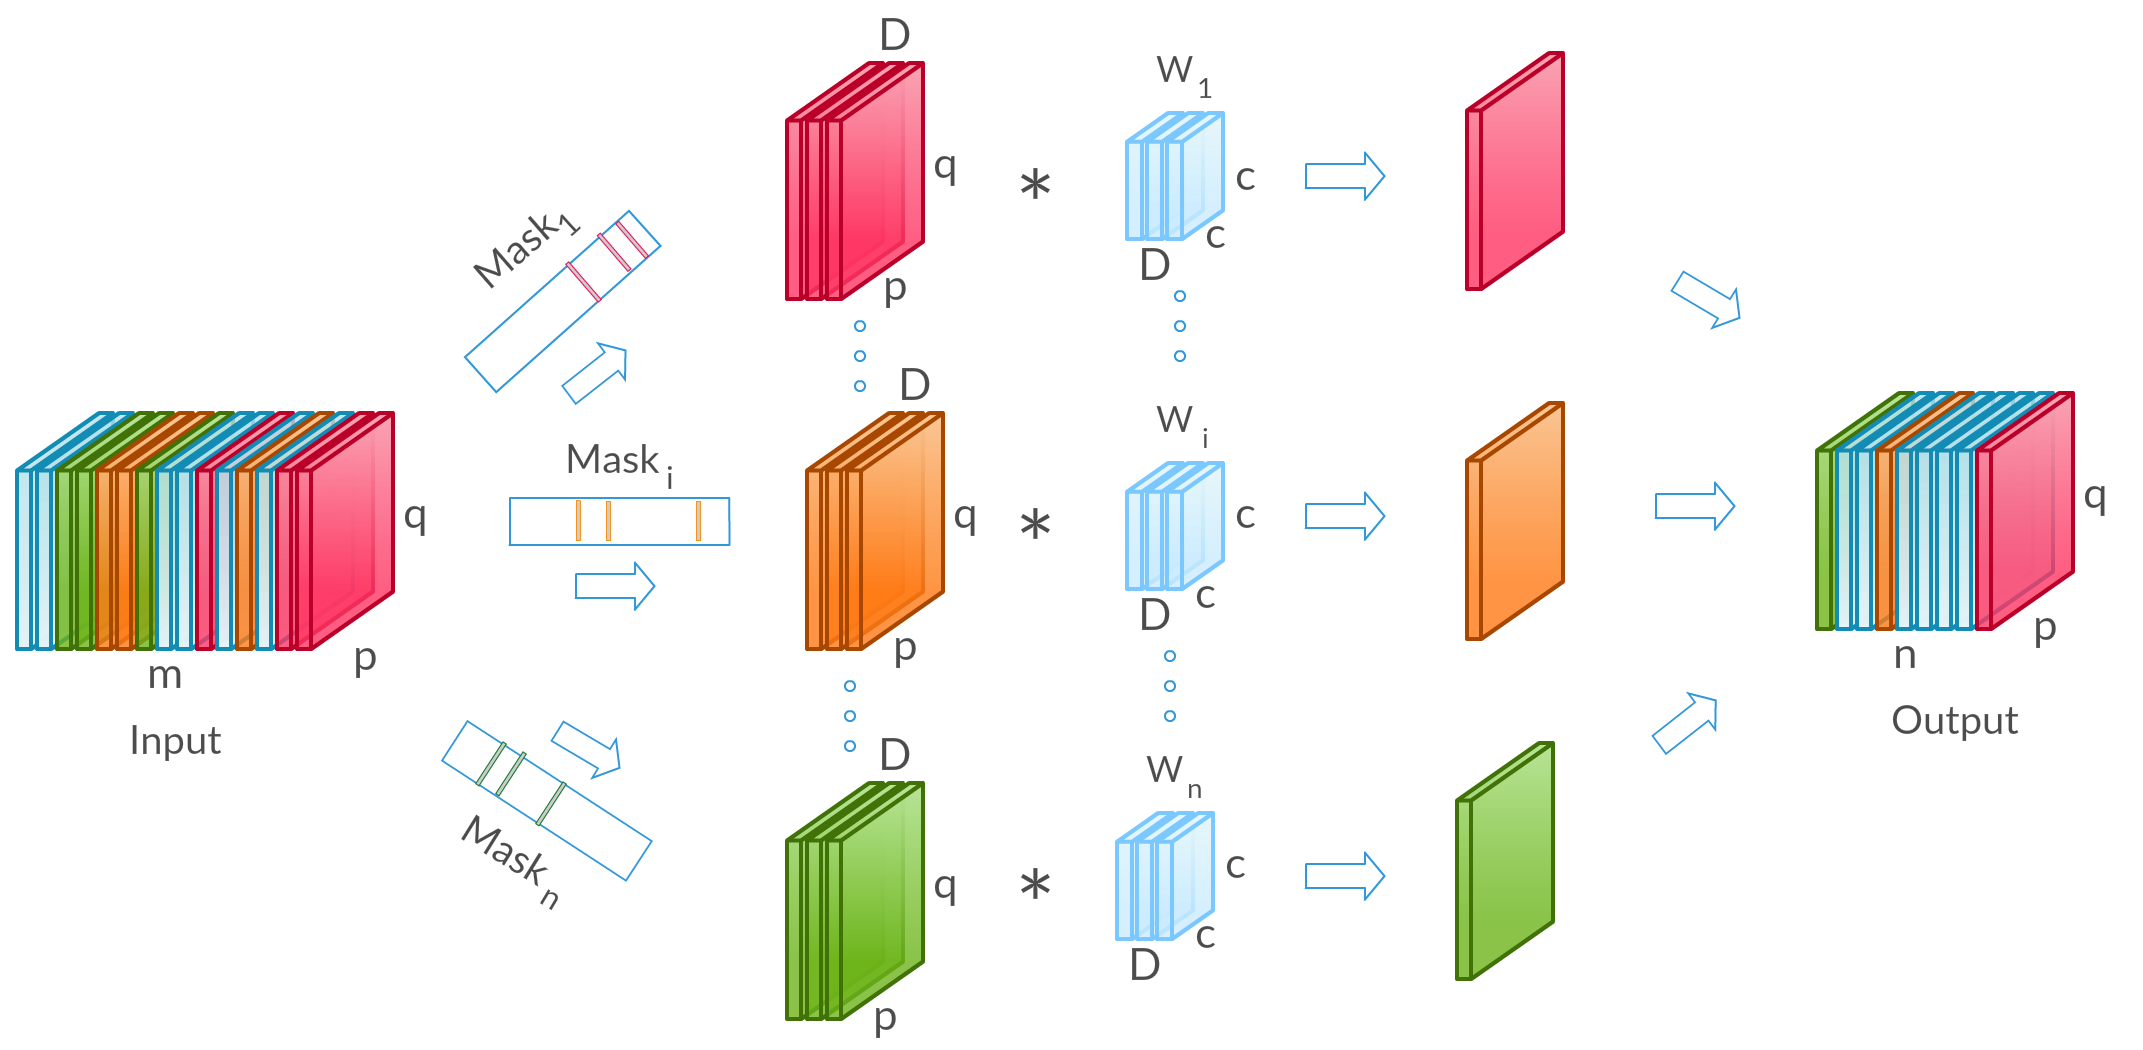
\includegraphics[width=1.0\textwidth]{figures/Expander.png}

\caption{The proposed fast convolution algorithm for X-Conv layer. We represent all the non-zero filters in the weight matrix of the X-Conv layer as a compressed dense matrix of $D$ channels. The algorithm starts by selecting $D$ channels from input (with replacement) using a mask created while initializing the model. The output is computed by convolving these selected channels with the compressed weight matrices.}
\label{fig:efficientmatrix}

\end{figure*}

\subsection{Measures of Connectivity}

\noindent In this subsection, we describe some connectivity properties of Expander graphs (see \cite{salil2012pseudo}, for the proofs). These will be used to prove the properties of sensitivity and mixing of random walks in X-Nets.\\

\noindent {\bf Expansion:} For every subset $S \subseteq V$ of size $\leq \alpha |V|$ ($\alpha \in (0,1)$ depends on the construction), let $N(S)$ be the set of neighbors. Then $|N(S)| \geq K |S|$ for $K\approx D$. That is, the neighbors of the vertices in $S$ are almost distinct. It is known that random expanders have expansion factor $K \approx D$ (see Theorem 4.4 in \cite{salil2012pseudo}).\\

\noindent {\bf Small Diameter:} The diameter of a graph is the length of the longest path among all shortest paths. If $G(U,V,E)$ is a $D$-regular expander with expansion factor $K > 1$ and diameter $d$, then  $d\leq O(\log n )$. This bound on the diameter implies that for any pair of vertices, there is a path of length $O(\log n)$ in the graph.\\

\noindent {\bf Mixing of Random Walks:} Random walks in the graph quickly converge to the uniform distribution over nodes of the graph. If we start from any vertex and keep moving to a random neighbor, in $O(\log n)$ steps the distribution will be close to uniform over the set of vertices.

\subsection{Sensitivity of X-Nets}

\noindent X-Nets have multiple layers, each of which have connections derived from an expander graph. We can guarantee that the output nodes in such a network are sensitive to all the input nodes.\\

\begin{theorem}[Sensitivity of X-Nets]\label{thm:conn}
Let $n$ be the number of input as well as output nodes in the network and $G_1,G_2,\cdots, G_t$ be $D$ regular bipartite expander graphs with $n$ nodes on both sides. Then  
every output neuron is sensitive to every input in a Deep X-Net defined by $G_i$'s with depth $t = O( \log n)$.

Proof: For every pair of input and output $(u,v)$, we show that there is a path in the X-Net. The proof is essentially related to the the fact that expander graphs have diameter $O(\log n)$. A detailed proof can be found in the Appendix B.
\end{theorem}

\noindent Next, we show a much stronger connectivity property known as mixing for the X-Nets. The theorem essentially says that the number of edges between subsets of input and output nodes is proportional to the product of their sizes. This result implies that the connectivity properties are uniform and rich across all nodes as well as subsets of nodes of the same size. Simply put, all nodes tend to have equally rich representational power.\\ 

\begin{theorem}[Mixing in X-Nets]
Let $n$ be the number of input as well as output nodes in the network and $G$ be $D$ regular bipartite expander graph with $n$ nodes on both sides. Let $S,T$ be subsets of input and output nodes in the X-Net layer defined by $G$. The number of edges between $S$ and $T$ is $\approx D|S||T|/n$.

Proof: A detailed proof is provided in the Appendix B.
\end{theorem}

\section{Efficient Algorithms}\label{sec:implementation}
 
\noindent In this section, we present efficient algorithms of X-Conv layers. Our algorithms achieve speedups and save memory in the training as well as the inference phase. This enables one to experiment with significantly wider and deeper networks given  memory and runtime constraints.
We exploit the structured sparsity of expander graphs to design fast algorithms.  We propose two methods of training X-Nets, both requiring substantially less memory and computational cost than their vanilla counterparts: \\1) Using Sparse Representations \\2) Expander-Specific Fast Algorithms.

\subsection{Using Sparse Representation}

\noindent The adjacency matrices of expander graphs are highly sparse for $D << n$. Hence, we can initialize a sparse matrix with non-zero entries corresponding to the edges of the expander graphs. Unlike most pruning techniques, the sparse connections are determined before training phase, and stay fixed. Dense-Sparse convolutions are easy to implement, and are supported by most deep learning libraries. CNN libraries like Cuda-convnet\cite{cudaconvnet} support such random sparse convolution algorithms.

 \begin{algorithm}[t]
 \textbf{Algorithm 1: } Fast Algorithm for Convolutions in X-Conv Layer\\
 \begin{algorithmic}[1]
 \State For every vertex $v \in \{1,\cdots, n\}$, let $N(v,i)$ denote the $i$th neighbor of $v$ ($i \in \{1,\cdots, D\}$).
 \State Let $K_v$ be the $c\times c \times D \times 1$ sized kernel associated with the $v$th output channel.
 \State Let $O_v[x,y]$ be the output value of the $v$th channel at the position $x,y$.
 \For{$v$= 1 to n}
     \State $O_v[x,y] = K_v * \textit{Mask}_{N(v,1),\cdots N(v,D)}(I)[x,y]$.
 \EndFor
 \end{algorithmic}
 \label{alg:cnnalgo}
 \end{algorithm}
 
 
\subsection{X-Net based Fast Dense Convolution}
\noindent Next, we present fast algorithms that exploit the sparsity of expander graphs.\\ %Moreover, our algorithm for X-Conv layers works for random expanders as well.

\noindent {\bf X-Conv:} In an X-Conv layer, every output channel is only sensitive to $out$ rom input channels. We propose to use a mask to select $D$ channels of the input, and then convolve with a $c \times c \times D \times 1$ kernel, obtaining a single channel per filter in the output. The mask is obtained by choosing D samples uniformly (without replacement) from the set $\{1,\cdots N\}$, where $N$ is the number of input channels. The mask value is $1$ for each of the selected $D$ channels and $0$ for others (see Algorithm \ref{alg:cnnalgo}). This is illustrated in Figure \ref{fig:efficientmatrix}. There has been recent work about fast CUDA implementations called Block-Sparse GPU Kernels\cite{blocksparse}, which can implement this algorithm efficiently.

\section{Experiments and Results}\label{sec:experiments}
\begin{figure}
\centering
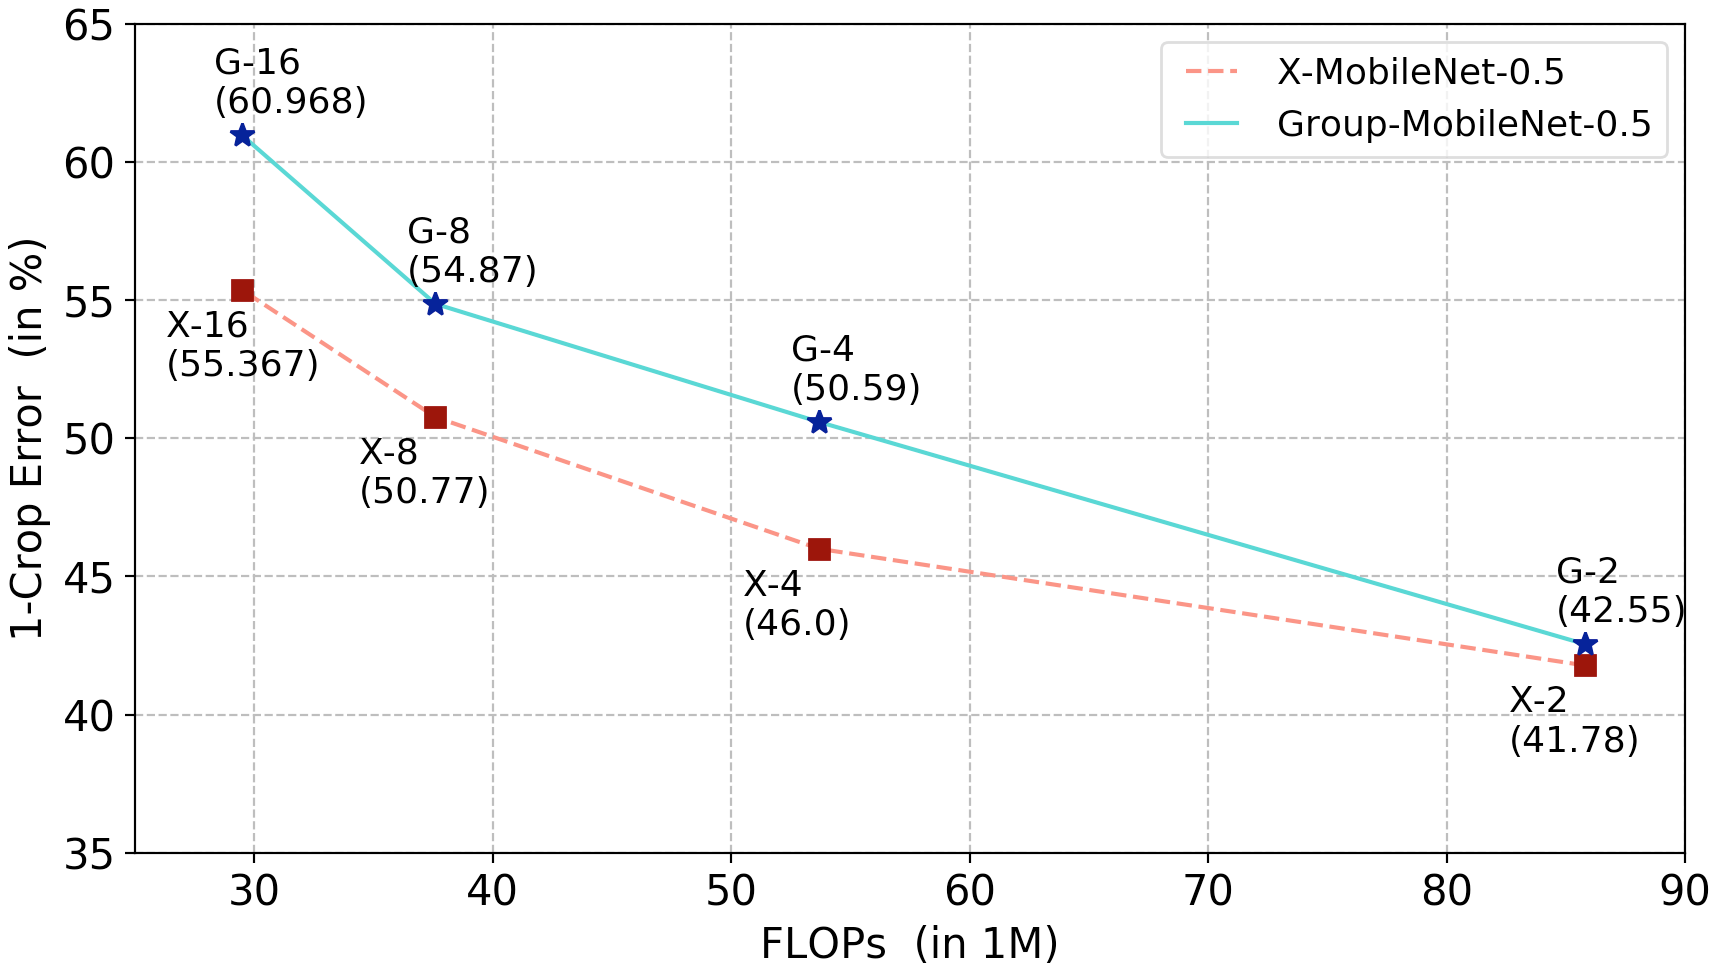
\includegraphics[width=0.55\textwidth]{figures/mobilenet.png}
\caption{Comparison between Grouped convolutions and X-Conv using MobileNet architecture trained on ImageNet. X-$d$ or G-$d$ represents the 1x1 conv layers are compressed by $d$ times using X-Conv or Groups. We observe X-MobileNets beat Group-MobileNet by 4\% in accuracy on increasing sparsity.}
\label{fig:mobilenet}
\end{figure}
\noindent In this section, we benchmark and empirically demonstrate the effectiveness of X-Nets on a variety of CNN architectures. Our code is available at: \url{https://github.com/DrImpossible/Deep-Expander-Networks}. 
\subsection{Comparison with Grouped Convolution}
\label{sec:group}


\noindent First, we compare our Expander Convolutions (X-Conv) against Grouped Convolutions (G-Conv). We choose G-Conv as it is a popular approach, on which a lot of concurrent works \cite{zhang2018shufflenet} have developed their ideas. G-Conv networks have the same sparsity as X-Conv networks but lack only the connectivity property. This will test whether increasing connectivity increases accuracy, i.e does a graph without good connectivity properties provides worse accuracy? We choose MobileNet as the base model for this experiment, since it is the state-of-the-art in efficient CNN architectures.\\
\begin{figure*}[t] 
\begin{tabular}{cc}
 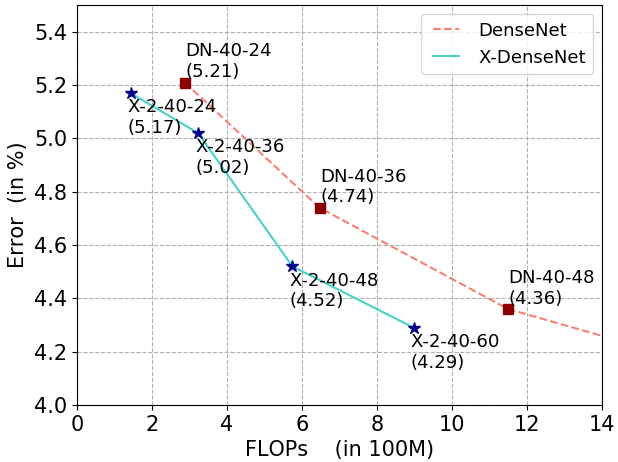
\includegraphics[width=0.5\textwidth]{figures/cifar10flops.png}  & 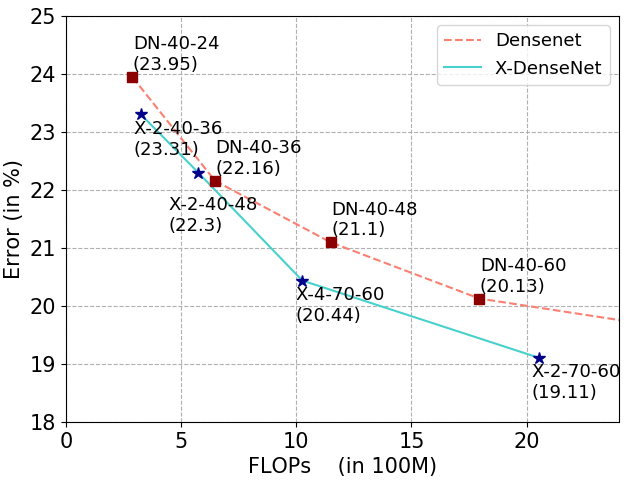
\includegraphics[width=0.5\textwidth] {figures/cifar100flops.png} \\
\\
(a) CIFAR10 & (b) CIFAR100 \\
\end{tabular}

\caption{We show the error as a function of \#FLOPs during test-time (below) for DenseNet-BC with X-DenseNet-BCs on CIFAR10 and CIFAR100 datasets. We observe X-DenseNet-BCs achieve better performance tradeoffs over DenseNet-BC models. For each datapoint, we mention the X-C-D-G notation (see Section \ref{sec:denres}) along with the accuracy.
}

\label{fig:cifar}
\end{figure*}
\noindent We compare X-Conv against grouped convolutions using MobileNet-0.5 on the ImageNet classification task. We replace the $1\times 1$ convolutional layers in MobileNet-0.5 with X-Conv layers forming X-MobileNet-0.5. Similarly, we replace them with G-Conv layers to form Group-MobileNet-0.5. Note that we perform this only in layers with most number of parameters (after the 8th layer as given in Table 1 of \cite{howard2017mobilenets}). We present our results in Figure \ref{fig:mobilenet}. The reference original MobileNet-0.5 has an error of 36.6\% with a cost of 150M FLOPs. Additional implementation details are given in the supplementary material.\\

\noindent We can observe that X-MobileNets beat Group-MobileNets by over 4\% in terms of accuracy when we increase sparsity. This also demonstrates that X-Conv can be used to further improve the efficiency of even the most efficient architectures like MobileNet.

\subsection{Comparison with Efficient CNN Architectures}
\label{sec:denres}

\noindent In this section, we test whether Expander Graphs can improve the performance trade-offs even in state-of-the-art architectures such as DenseNet-BCs \cite{huang2017densely} and ResNets\cite{he2016deep} on the ImageNet \cite{deng2009imagenet} dataset. We additionally train DenseNet-BCs on CIFAR-10 and CIFAR-100 \cite{krizhevsky2009learning} datasets to demonstrate the robustness of our approach across datasets.\\ 

\noindent Our X-ResNet-C-D is a $D$ layered ResNet that has every layer except the first and last replaced by an X-Conv layer that compresses connections between it and the previous layer by a factor of $C$. We compare across various models like ResNets-34,50,101. Similarly, our X-DenseNet-BC-C-D-G architecture has depth $D$, and growth rate $G$. We use DenseNet-BC-121-32,169-32,161-48,201-32 as base models. These networks have every layer except the first and last replaced by an X-Conv layer that compresses connections between it and the previous layer by a factor of $C$. More details are provided in the supplementary material.\\

\begin{figure}
\centering
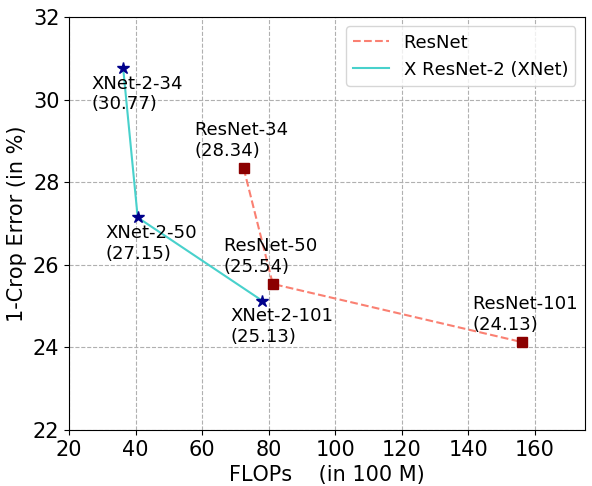
\includegraphics[width=0.55\textwidth]{figures/resnet.png}
\caption{We show the error as a function of \#FLOPs to compare between ResNet and X-ResNet on the ImageNet dataset. We observe X-ResNets achieve better performance tradeoffs over original ResNet models.}
\label{fig:resnet}
\end{figure}
   
 
\begin{table}
\centering
\begin{tabular}{|l|c|c|}
\hline
{\bf Model} & {\bf Accuracy}  & {\bf \#FLOPs}\\
\hline
ResNet &   & {\bf(in 100M)}\\
\hline
X-ResNet-2-34 & 69.23\%  & 35\\
X-ResNet-2-50 & {\bf 72.85\%}  & {\bf 40}\\
ResNet-34 & 71.66\%  & 70\\
X-ResNet-2-101 & {\bf 74.87\%}  & {\bf 80}\\
ResNet-50 & 74.46\%  & 80\\
ResNet-101 & 75.87\%  & 160\\
\hline
DenseNet-BC &  &   \\
\hline
X-DenseNet-BC-2-121 & 70.5\% & 28\\
X-DenseNet-BC-2-169 & 71.7\% & 33\\
X-DenseNet-BC-2-201 & 72.5\% & 43\\
X-DenseNet-BC-2-161 & {\bf 74.3\%} & {\bf 55}\\
DenseNet-BC-121 & 73.3\% & 55\\
DenseNet-BC-169 & 74.8\% & 65\\
DenseNet-BC-201 & 75.6\% & 85\\
DenseNet-BC-161 & 76.3\% & 110\\
\hline
\end{tabular}
      \caption{Results obtained by ResNet and DenseNet-BC models on ImageNet dataset, ordered by \#FLOPs. or each datapoint, we use the X-C-D-G notation (see Section \ref{sec:denres}) along with the accuracy.}
\label{tab:imagenet}
\end{table}
\subsection{Comparison with Pruning Techniques}
\label{sec:prun}

\noindent We plot the performance tradeoff of X-ResNets against ResNets in Figure \ref{fig:resnet} . We achieve significantly better performance tradeoffs compared to the original model. More specifically, we can reduce the \#FLOPs in ResNets by half while incurring only 1-1.5\% decrease in accuracy. Also, we can compare models with similar \#FLOPs or accuracy with the help of Table \ref{tab:imagenet}. We observe that  X-ResNet-2-50 has 43\% fewer FLOPs than ResNet-34, but achieves a 1\% improvement in accuracy against it. Similarly, X-DenseNet-BC-2-161 has similar \#FLOPs as DenseNet-BC-121, but achieves a 1\% improvement in accuracy. \\ 

\noindent To further prove the robustness of our approach on DenseNet-BC, we test the same on CIFAR10 and CIFAR100, and plot the tradeoff curve in Figure \ref{fig:cifar}.
We observe that we can achieve upto 33\% compression keeping accuracy constant on CIFAR-10 and CIFAR-100 datasets. \\

\noindent We compare our approach with methods which prune the weights during or after training. Our method can be thought of as constraining the weight matrices with a well studied sparse connectivity pattern even before the training starts. This results in fast training for the compact X-Conv models, while the trained pruning techniques face the following challenges: \\

\noindent 1) Slow initial training due to full dense model.\\
\noindent 2) Several additional phases of pruning and retraining.\\

\noindent Hence they achieve the compactness and runtime efficiency only in test time. Nevertheless we show similar sparsity can be achieved by our approach without explicitly pruning. We benchmark on VGG16 and AlexNet architectures since most previous results in the pruning literature have been reported on these architectures. In Table \ref{tab:cifar_fullcomp}, we compare two X-VGG-16 models against existing pruning techniques. We achieve comparable accuracies to the previous state-of-the-art model with 50\% fewer parameters and \#FLOPs. Similarly, in Table \ref{tab:imagenet_fullcomp} we compare X-AlexNet with trained pruning techniques on the Imagenet dataset. Despite having poor connectivity due to parameters being concentrated only in the last three fully connected layers, we achieve similar accuracy to AlexNet model using only 7.6M-9.7M parameters out of 61M, comparable to the state-of-the-art pruning techniques which have upto 3.4M-5.9M parameters. Additionally, it is possible to improve compression by applying pruning methods on our compact architectures, but pruning X-Nets is out of the scope of our current work.\\
\begin{table}[t]%{0.8\textwidth}
  \centering
\begin{tabular}{|l|c|c|}
\hline
{\bf Method} & {\sc { \bf Accuracy}} & {\bf \#Params} \\
 %&  &  & {\bf Speedup }?\\
\hline
Li et al. \cite{li2016pruning} & 93.4\%  & 5.4M \\
Liu et al. \cite{liu2017learning} &  93.8\% & 2.3M \\
\hline
X-VGG16-1 & 93.4\%  & 1.65M (9x) \\
X-VGG16-2 & 93.0\%  & 1.15M (13x) \\
\hline
VGG16-Orig &  94.0\% & 15.0M \\
\hline
\end{tabular}
\captionof{table}{Comparison with other methods on CIFAR-10 dataset using VGG16 as the base model. We significantly outperform popular compression techniques, achieving similar accuracies with upto 13x compression rate.}
\label{tab:cifar_fullcomp}
%\vspace{-0.6cm}
  \end{table}
  
\begin{table}[t]%{0.8\textwidth}
    \centering
\begin{tabular}{|l|c|c|}
\hline
{\bf Method} & {\bf Accuracy} & {\bf \#Params}\\ \hline
Network Pruning & & \\
\hline
Collins et al.\cite{collins2014memory} & 55.1\% & 15.2M \\
Zhou et al. \cite{zhou2016less} & 54.4\% & 14.1M \\
Han et al. \cite{han2015deep} &  57.2\% & 6.7M  \\
Han et al. \cite{han2015deep} & 57.2\% & 6.7M \\
 Srinivas et al. \cite{srinivas2017training} & 56.9\% & 5.9M \\
Guo et al. \cite{guo2016dynamic} & 56.9\% & 3.4M  \\
X-AlexNet-1 & 55.2\% & 7.6M  \\
X-AlexNet-2 & 56.2\% & 9.7M \\
\hline
AlexNet-Orig & 57.2\% & 61M \\
\hline
\end{tabular}
\captionof{table}{Comparison with other methods on ImageNet-2012 using AlexNet as the base model. We are able to achieve comparable accuracies using only 9.7M parameters.}
\label{tab:imagenet_fullcomp}
%\vspace{-0.6cm}
    \end{table}
  

\subsection{Stability of Models}
\noindent We give empirical evidence as well as a theoretical argument regarding the stability of our method. For the vanilla DNN training, the weights are randomly initialized, and randomized techniques like dropouts, augmentation are used. Hence there is some randomness present and is well accepted in DNN literature prior to our method. We repeat experiments on different datasets (Imagenet and CIFAR10) and architectures (VGG, DenseNet and MobileNet0.5) to empirically show that the accuracy of expander based models has variance similar to vanilla DNN training over multiple runs.\\

\noindent We repeated the experiments with independent sampling of random expanders on the VGG and DenseNet baselines on the CIFAR10 dataset. The results can be seen in Table~\ref{tab:cifar}. It is noted that the accuracy values changes only by less than $0.3$\% across runs and the standard deviation of expander method is also comparable to the vanilla DNN training.\\

\noindent We also repeated experiments of our main result, which is the comparison with grouped convolutions on ImageNet dataset. We rerun the experiment with MobileNet0.5 feature extractor twice with Groups and the expander method. As can be seen from Table~\ref{tab:imgnet}, the accuracy variations are comparable between the two models, and it is less than 1\%.\\

\begin{table}[!thb]
%\vspace{-2em}
\begin{minipage}{.5\linewidth}
\centering
\scalebox{0.9}{
\begin{tabular}{|l|c|c|c|c|}
\hline
{\bf Model} & {\bf Accuracy\%} & {\bf Max\%} & {\bf Min\%}\\
\hline
VGG & 93.96$\pm0.12$ & 94.17 & 93.67 \\
\hline
X-VGG-1 & 93.31$\pm0.18$ & 93.66 & 93.06 \\
X-VGG-2 & 92.91$\pm0.19$ & 93.26 & 92.69 \\
\hline
XDNetBC-40-24 & 94.41$\pm$0.19 & 94.63 & 94.18 \\
XDNetBC-40-36 & 94.98$\pm$0.14 & 95.21 & 94.84 \\
XDNetBC-40-48 & 95.49$\pm$0.15 & 95.65 & 95.28 \\
XDNetBC-40-60 & 95.75$\pm$0.07 & 95.81 & 95.68 \\

\hline
\end{tabular}}
%\vspace{0.5em}
\caption{The accuracies (mean $\pm$ stddev) of various models over 10 training runs on CIFAR-10 dataset.} \label{tab:cifar}
\end{minipage}%
\hfill
 \begin{minipage}{.45\linewidth}
 \centering
 \scalebox{0.9}{
\begin{tabular}{|c|c|c|}
\hline
{\bf MobileNet} & {\bf Mean} & {\bf Range}\\
{\bf Variant}  & {\bf Accuracy} & {\bf (Max-Min)}\\
\hline
Base & $63.39\%$ & $0.11\%$\\

\hline
G2 & $57.45~\%$ & $0.06~\%$\\
X2 & \bf{$58.22~\%$} & $ 0.14~\%$\\
\hline
G4 & $49.41~\%$ & $0.55~\%$\\
X4 & \bf{$54.00~\%$} & $0.53~\%$\\
\hline
G8 & $45.13~\%$ & $0.03~\%$\\
X8 & \bf{$49.23~\%$} & $0.60~\%$\\
\hline
G16 & $39.03~\%$ & $0.64~\%$\\
X16 & \bf{$44.63~\%$} & $0.18~\%$\\
\hline
\end{tabular}}
%\vspace{0.5em}\\
\caption{The mean accuracy and range of variation over  2 runs of MobileNet0.5 variants on ImageNet dataset.} \label{tab:imgnet}
\end{minipage}%
%\vspace{-3em}
\end{table}
\noindent A theoretical argument also concludes that choosing random graphs doesn't degrade stability. It is a well known result (See Theorem 4.4 in  \cite{salil2012pseudo}) in random graph theory, that graphs chosen randomly are well connected with overwhelmingly high probability (with only inverse exponentially small error, due to the Chernoff's Tail bounds) and satisfies the Expander properties. Hence the chance that for a specific run, the accuracy gets affected due to the selection of a particularly badly connected graph is insignificant.

\subsection{Training Wider and Deeper  networks}\label{sec:ultrawide}

\begin{figure*}[t]
\begin{tabular}{cc}

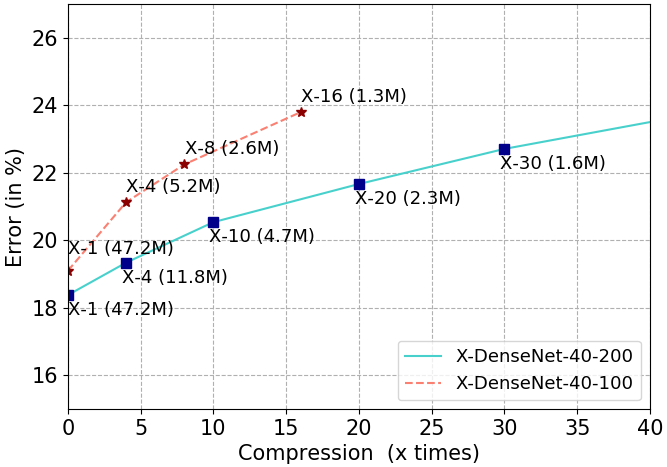
\includegraphics[width=0.5\textwidth]{figures/ultrawide.png}  & 
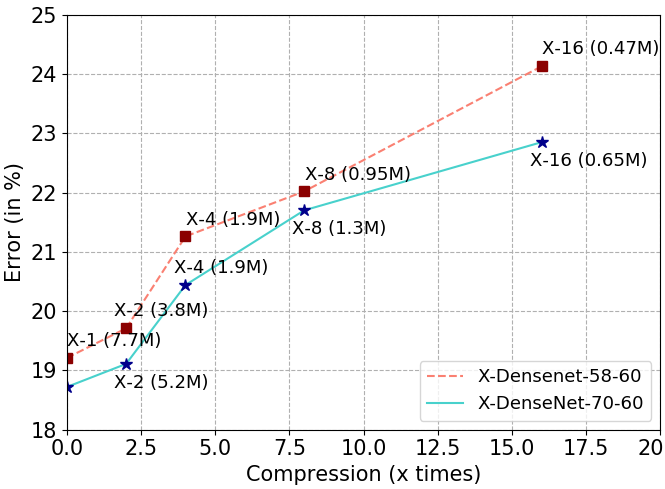
\includegraphics[width=0.5\textwidth] {figures/ultradeep.png}\\
(a) Effect of Width  & (b) Effect of Depth \\
\end{tabular}
\caption{We show the performance tradeoff obtained on training significantly wider and deeper networks on CIFAR-100 dataset. Every datapoint is X-$C$ specified along with the number of parameters, $C$ being the compression factor. We show that training wider or deeper networks along with more  compression using X-Nets achieve better accuracies with upto two-thirds of the total parameter and FLOPs on CIFAR-100 dataset. }
\label{fig:deepnet}
\end{figure*}

\noindent Since X-Nets involve constraining the weight matrices to sparse connectivity patterns before training, the fast algorithms can make it possible to utilize memory and runtime efficiently in training phase. This makes it possible to train significantly deeper and wider networks. Note the contrast with pruning techniques, where it is necessary to train the full, bulky model, inherently limiting the range of models that can be compressed.\\

\noindent Wide-DenseNets\footnote{https://github.com/liuzhuang13/DenseNet\#wide-densenet-for-better-timeaccuracy-and-memoryaccuracy-tradeoff} offered a better accuracy-memory-time trade-off. We increase the width and depth of these networks to train significantly wider and deeper networks. The aim is to study whether leveraging the effectiveness of X-Nets in this fashion can lead to better accuracies. \\
  
\noindent We widen and deepen the DenseNet-BC-40-60 architecture, increasing the growth rate from 60 to 100 and 200 respectively and compare the effect of increasing width on these new models. Similarly, we increase the depth from 40 to 58 and 70 to obtain deeper networks. We benchmark these approaches using CIFAR-100 dataset and present the results in Figure \ref{fig:deepnet}. \\

\noindent We have two interesting observations. First, the deeper X-DenseNet-BC-70-60 significantly outperforms X-DenseNet-BC-58-60 and wider X-DenseNet-40-200 outperforms X-DenseNet-BC-40-100 with fewer parameters for a wide range of $C$ values (Expander degree). \\

\noindent The second interesting observation is the decreasing slope of the curves. This  indicates that expander graph modeling seems to be effective on wider and deeper X-Nets i.e X-DenseNet-BC models suffer lesser penalty with increasing depth and width compression. This enables X-Nets to work at high compression rates of 30x, compressing DenseNet-BC-40-200 model from 19.9B FLOPs to 0.6B FLOPs with only $4.3\%$ drop in accuracy. We hope this preliminary investigation holds significant value in alleviating the constraint of GPU memory and resources.

\section{Summary}

\noindent We proposed a new network layer architecture for deep networks using expander graphs that give strong theoretical guarantees on connectivity. The resulting architecture (X-Net) is shown to be highly efficient in terms of both computational requirements and model size. In addition to being compact and computationally efficient, the connectivity properties of the network allow us to achieve significant improvements over the state-of-the-art architectures in performance on a parameter or run-time budget. In short, we show that the use of principled approaches that sparsify a model while maintaining global information flows can help in developing efficient deep networks. To the best of our knowledge, this is the first attempt at using theoretical results from graph theory in modeling connectivity to improve deep network architectures.
%--------------------------------------------------------
\chapter{Conclusions}
\label{ch:wrapup}
\noindent Convolutional Neural Networks (CNNs) have found applications in many vision-related domains ranging such as generic image-understanding to self-driving cars \cite{bojarski2016end}. However, deep neural networks are increasingly computationally and memory intensive, and need to work with embedded hardware which have limited energy and memory availability. To address this problem, we presented algorithms for improving the efficiency and accuracy of compressed deep networks. In this thesis, we developed three improvements over existing network compression literature. Distribution Aware Binary Networks, which offers a binary representation specific to the input weight distribution. Hybrid Binary Networks, where we demonstrated that binarizing the right areas in the network contributes significantly to the overall accuracy of the network and does not damage its speed-ups in Hybrid Binary Networks. Deep Expander Networks provided a principled method to prune networks before considering the training data. These methods share a common principle: utilizing over-parameterization in deep neural networks for developing fast, accurate and compact deep networks.\\

\noindent We first showed that binary networks have similar representation power as infinite-precision networks. We proposed a distribution-aware binary representation for layer-weights. Using dynamic programming, we came up with an algorithm for computing this representation efficiently. We got significant improvements on large-scale datasets, showing the efficacy of our algorithm. We provide inuitions and reductions to previous binarization techniques.\\

\noindent Secondly, we presented the idea that avoiding binarization of few select layers can restore the accuracy boost, while nearly maintaining the compression rates. We proposed a heuristic for selecting the layers to be binarized. We successfully weight-binarized the last layers without significant accuracy drops, a problem faced by previous works in this area.  We also showed that we can successfully combine  the  advantages  of  our  approach  with  other  architectural compression strategies, to obtain highly efficient models with negligible accuracy penalties. Overall, we asked the question: Where to binarize to augment our previously proposed binarization strategy.\\

\noindent There can be several possible directions to extend this work. We see promise in binary networks and hope to further develop binary representations which are competitive with floating point representations in accuracy.\\ 

\noindent Finally, we attack pruning in a novel fashion. We provide a principled approach for pruning before training by utilizing concepts from graph theory: particularly using expander graphs that give strong theoretical guarantees on connectivity. The resulting architecture (X-Net) is shown to be highly efficient in terms of both computational requirements and model size, achieve significant improvements over the state-of-the-art architectures in performance on a parameter or run-time budget. The principle used is: global information flows can be maintained even while sparsifying the model significantly, producing efficient deep networks.  We hope that this work motivates other approaches to utilize results from graph theory to develop efficient network architectures. Further interesting directions include using random graphs for architecture design, combine pruning and binarization to provide extremely compact networks, etc.
%--------------------------------------------------------
\chapter*{Related Publications}
\label{ch:relatedPubs}
\begin{itemize}
\item Ameya Prabhu, Vishal Batchu, Rohit Gajawada, Sri Aurobindo Munagala, Anoop Namboodiri \textbf{Hybrid Binary Networks: Optimizing for Accuracy, Efficiency and Memory}. \emph{IEEE Winter  conference on Applications of Computer Vision (WACV 2018)}, Lake tahoe, USA. (Oral)
\item Ameya Prabhu, Vishal Batchu, Sri Aurobindo Munagala, Rohit Gajawada, Anoop Namboodiri. \textbf{Distribution-Aware Binarization of Neural Networks for Sketch Recognition}. \emph{IEEE Winter  conference on Applications of Computer Vision (WACV 2018)}, Lake tahoe, USA. (Oral)
\item Ameya Prabhu*, Girish Varma*, Anoop Namboodiri. \textbf{Deep Expander Networks: Efficient Deep Networks from Graph Theory}. \emph{European Conference on Computer Vision (ECCV 2018)}, Munich, Germany. (Oral)
\end{itemize}
%\newcommand{\colvec}[1]{\left[ \begin{array}{c} #1 \end{array} \right]}
\newcommand{\matrx}[2]{{\left[ \begin{array}{#1} #2 \end{array} \right]}}

\newcommand{\myfor}{{\bf for }}
\newcommand{\myif}{{\bf if }}
\newcommand{\myelse}{{\bf else }}
\newcommand{\mythen}{{\bf then }}
\newcommand{\myloop}{{\bf loop }}
\newcommand{\mat}[1]{\mbox{$ {\bf {#1}} $}}
\newcommand{\myvec}[1]{{\vec{\bf {#1}}}}
\newcommand{\mypt}[1]{{\bar{\bf {#1}}}}

\newcommand{\ssp}{\vspace*{1.0cm}}
\newcommand{\hsp}{\vspace*{0.5cm}}
\def\grad{\nabla}

\newcommand{\figureplaceholder}{\centerline{\bf (figure goes here)}}

\newcommand{\argmin}[1]{\underset{#1}{\operatorname{argmin}}}

\newcommand{\bA}{\mathbf{A}}
\newcommand{\bB}{\mathbf{B}}
\newcommand{\bC}{\mathbf{C}}
\newcommand{\bD}{\mathbf{D}}
\newcommand{\bE}{\mathbf{E}}
\newcommand{\bF}{\mathbf{F}}
\newcommand{\bG}{\mathbf{G}}
\newcommand{\bH}{\mathbf{H}}
\newcommand{\bI}{\mathbf{I}}
\newcommand{\bJ}{\mathbf{J}}
\newcommand{\bK}{\mathbf{K}}
\newcommand{\bL}{\mathbf{L}}
\newcommand{\bM}{\mathbf{M}}
\newcommand{\bN}{\mathbf{N}}
\newcommand{\bO}{\mathbf{O}}
\newcommand{\bP}{\mathbf{P}}
\newcommand{\bQ}{\mathbf{Q}}
\newcommand{\bR}{\mathbf{R}}
\newcommand{\bS}{\mathbf{S}}
\newcommand{\bT}{\mathbf{T}}
\newcommand{\bU}{\mathbf{U}}
\newcommand{\bV}{\mathbf{V}}
\newcommand{\bW}{\mathbf{W}}
\newcommand{\bX}{\mathbf{X}}
\newcommand{\bY}{\mathbf{Y}}
\newcommand{\bZ}{\mathbf{Z}}

\newcommand{\bbf}{\mbox{\boldmath $f$}}



\newcommand{\bphi}{\mbox{\boldmath $\phi$}}


\newcommand{\bxi}{\mbox{\boldmath $\xi$}}
\newcommand{\bxh}{\hat{\mbox{\boldmath $x$}}}
\newcommand{\btheta}{\mbox{\boldmath $\theta$}}
\newcommand{\Psih}{\mbox{\boldmath $\hat{\Psi}$}}
\newcommand{\sgn}{\text{sign}}




\newcommand{\ba}{\mathbf{a}}
\newcommand{\bb}{\mathbf{b}}
\newcommand{\bc}{\mathbf{c}}
\newcommand{\bd}{\mathbf{d}}
\newcommand{\be}{\mathbf{e}}
\newcommand{\mybf}{\mathbf{f}}
\newcommand{\bg}{\mathbf{g}}
\newcommand{\bh}{\mathbf{h}}
\newcommand{\bi}{\mathbf{i}}
\newcommand{\bj}{\mathbf{j}}
\newcommand{\bk}{\mathbf{k}}
\newcommand{\bl}{\mathbf{l}}
\newcommand{\bm}{\mathbf{m}}
\newcommand{\bn}{\mathbf{n}}
\newcommand{\bo}{\mathbf{o}}
\newcommand{\bp}{\mathbf{p}}
\newcommand{\bq}{\mathbf{q}}
\newcommand{\br}{\mathbf{r}}
\newcommand{\bs}{\mathbf{s}}
\newcommand{\bt}{\mathbf{t}}
\newcommand{\bu}{\mathbf{u}}
\newcommand{\bv}{\mathbf{v}}
\newcommand{\bw}{\mathbf{w}}
\newcommand{\bx}{\mathbf{x}}
\newcommand{\by}{\mathbf{y}}
\newcommand{\bz}{\mathbf{z}}

\newcommand{\bzero}{\mathbf{0}}
\newcommand{\bone}{\mathbf{1}}
\newcommand{\bbeta}{\mathbf{\beta}}
\newcommand{\cov}{\mathrm{cov}}
\newcommand{\var}{\mathrm{var}}

\newcommand{\expect}[1]{\left<{#1}\right>}

% I HATE LATEX.
\newcommand{\bLambda}{\mbox{\boldmath$\Lambda$}}
\newcommand{\bSmallLambda}{\mbox{\boldmath\scriptsize$\Lambda$}}
\newcommand{\blambda}{\mbox{\boldmath$\lambda$}}
\newcommand{\bomega}{\mbox{\boldmath$\omega$}}
\newcommand{\bSigma}{\mbox{\boldmath$\Sigma$}}
\newcommand{\bmu}{\mbox{\boldmath$\mu$}}
\newcommand{\bPhi}{\mbox{\boldmath$\Phi$}}
\newcommand{\balpha}{\mbox{\boldmath$\alpha$}}


\newcommand{\ynew}{y_{\mathit{new}}}
\newcommand{\xnew}{x_{\mathit{new}}}
\newcommand{\bxnew}{\mathbf{x}_{\mathit{new}}}

\newcommand{\cD}{\mathcal{D}}
\newcommand{\cL}{\mathcal{L}}
\newcommand{\cF}{\mathcal{F}}
\newcommand{\cM}{\mathcal{M}}
\newcommand{\cN}{\mathcal{N}}

% \newcommand{\hA}{\hat{A}}
% \newcommand{\hp}{\hat{p}}
% \newcommand{\hq}{\hat{q}}
% \newcommand{\hx}{\hat{x}}
% \newcommand{\hv}{\hat{v}}
% \newcommand{\hF}{\hat{F}}
% \newcommand{\hM}{\hat{M}}
%
% \newcommand{\pC}{\bar{C}}
% \newcommand{\pS}{\bar{S}}
% \newcommand{\pa}{\bar{a}}
% \newcommand{\pb}{\bar{b}}
% \newcommand{\pc}{\bar{c}}
% \newcommand{\pd}{\bar{d}}
% \newcommand{\pe}{\bar{e}}
% \newcommand{\pf}{\bar{f}}
% \newcommand{\pl}{\bar{l}}
% \newcommand{\pp}{\bar{p}}
% \newcommand{\pq}{\bar{q}}
% \newcommand{\pr}{\bar{r}}
% \newcommand{\ps}{\bar{s}}
% \newcommand{\pu}{\bar{u}}
% \newcommand{\px}{\bar{x}}
% \newcommand{\py}{\bar{y}}
% \newcommand{\pz}{\bar{z}}

% \newcommand{\va}{\vec{a}}
% \newcommand{\vb}{\vec{b}}
% \newcommand{\vc}{\vec{c}}
% \newcommand{\vd}{\vec{d}}
% \newcommand{\vg}{\vec{g}}
% \newcommand{\vf}{\vec{f}}
% \newcommand{\vm}{\vec{m}}
% \newcommand{\vn}{\vec{n}}
% \newcommand{\vp}{\vec{p}}
% \newcommand{\vq}{\vec{q}}
% \newcommand{\vr}{\vec{r}}
% \newcommand{\vs}{\vec{s}}
% \newcommand{\vt}{\vec{t}}
% \newcommand{\vu}{\vec{u}}
% \newcommand{\vv}{\vec{v}}
% \newcommand{\vw}{\vec{w}}
% \newcommand{\vx}{\vec{x}}
% \newcommand{\vy}{\vec{y}}
% \newcommand{\vz}{\vec{z}}
% \newcommand{\vtau}{\vec{\tau}}

\newcommand{\real}{\mathbb{R}}
\newcommand{\natl}{\mathbb{N}}

\newcommand{\Uniform}{\mathcal{U}}
\newcommand{\Gaussian}{\mathcal{N}}

% \newcommand{\tA}{\tilde{A}}
% \newcommand{\tb}{\tilde{b}}
% \newcommand{\tB}{\tilde{B}}
% \newcommand{\tw}{\tilde{w}}
% \newcommand{\tbw}{\tilde{\mathbf{w}}}
% \newcommand{\tbW}{\tilde{\mathbf{W}}}
% \newcommand{\tbx}{\tilde{\mathbf{x}}}
% \newcommand{\tbX}{\tilde{\mathbf{X}}}
% \newcommand{\tby}{\tilde{\mathbf{y}}}
% \newcommand{\tbV}{\tilde{\mathbf{V}}}
% \newcommand{\tW}{\tilde{W}}
% \newcommand{\tx}{\tilde{x}}
% \newcommand{\ty}{\tilde{y}}
% \newcommand{\tX}{\tilde{X}}
% \newcommand{\btz}{\tilde{\mathbf{z}}}

\newcommand{\tLambda}{\tilde{\Lambda}}

\newcommand{\order}{\mathcal{O}}
%\newcommand{\choose}[2]{\left(\begin{array}{c}{#1}\\{#2}\right)}

\newcommand{\heads}{\mathsf{heads}}
\newcommand{\tails}{\mathsf{tails}}
\newcommand{\model}{\mathsf{model}}
\newcommand{\data}{\mathsf{data}}

%--------------------------------------------------------
%%% Optional appendix
\appendix
\chapter{Binary Networks: Appendix}
\label{ch:apndx1}

This appendix consists of additional details regarding Chapters 3 and 4.

\section{Optimal representation of $\widetilde{\mathbf{W}}$}
\newtheorem{name2}{Theorem 2.}
\begin{name2}
\label{approx}
The optimal binary weight $\widetilde{\mathbf{W}}$ which minimizes the error function $\mathbf{J}$ is
$$\widetilde{\mathbf{W}} = \alpha \mathbf{e} + \beta \mathbf{(1-e)} \\$$
where $\; \alpha =\frac{\mathbf{W}^{T}\mathbf{e}}{K} \;$, $\; \beta = \frac{\mathbf{W}^{T}\mathbf{(1-e)}}{n-K} \;$ and the optimal $\mathbf{e}^\ast$ is $\;  \mathbf{e}^\ast  = \underset{\mathbf{e},K}{\mathrm{argmax}} (\frac{ \parallel \mathbf{W}^T\mathbf{e} \parallel^{2}}{K} + \frac{\parallel \mathbf{W}^{T}\mathbf{(1-e)}\parallel^{2}}{n-K})$
\end{name2}

{\bf Proof:} The approximated weight vector $\widetilde{\mathbf{W}}=[\alpha \alpha \ldots \beta  \alpha  \ldots \beta \beta$] can be decomposed as:
$$[\alpha \alpha \ldots \beta  \alpha  \ldots \beta \beta] = \alpha \cdot [ 1 1 \ldots 0  1  \ldots 0 0 ] + \beta \cdot [ 0 0 \ldots 1  0  \ldots 1 1 ]$$ 
where without loss of generality, $\mathbf{e} \in \{0,1\}^n, \mathbf{e}^T\mathbf{e} >  0, \mathbf{e} \in \{0,1\}^n, (\mathbf{1-e})^T(\mathbf{1-e}) >  0$ and $\alpha,\beta \in \mathbb{R}$. This is because the trivial case where $\mathbf{e} = \mathbf{0}$ or $\mathbf{e} = \mathbf{1}$ is covered by substituting  $\alpha = \beta$ instead and the equation is independent of $\mathbf{e}$.
We have to find the values of $\alpha$ and $\beta$ which would be the best approximation of this vector. \\
Let us define the error function $\mathbf{J} = \mathbf{W} - (\alpha \cdot \mathbf{e} + \beta \cdot (\mathbf{1-e}))$.
We have to minimize $\parallel \mathbf{J} \parallel^2 = \mathbf{E}$, where:
\begin{dmath}
\mathbf{E} = (\mathbf{W} - (\alpha \cdot \mathbf{e} + \beta \cdot (\mathbf{1-e})))^T(\mathbf{W} - (\alpha \cdot \mathbf{e} + \beta \cdot (\mathbf{1-e}))) \end{dmath}
\begin{dmath}
\mathbf{E} = \mathbf{W}^{T}\mathbf{W} + \alpha^2 \cdot \mathbf{e}^T\mathbf{e} + \beta^2\mathbf{(1-e)}^T \mathbf{(1-e)} \\ - 2\alpha \cdot \mathbf{W}^T\mathbf{e} - 2\beta \cdot \mathbf{W}^T(\mathbf{1-e}) + 2\alpha \beta \mathbf{e}^{T}\mathbf{(1-e)}
\end{dmath}
where $\mathbf{e}^T\mathbf{e} = K$, then $(\mathbf{1-e})^T(\mathbf{1-e}) = n-K$ and $\mathbf{e}^{T}\mathbf{(1-e)} = 0$. Substituting these in, we get
\begin{equation}\mathbf{E} =  \mathbf{W}^{T}\mathbf{W} + \alpha^2 K + \beta^2 (n-K) -\\ 2\alpha \cdot \mathbf{W}^T\mathbf{e} - 2\beta \cdot \mathbf{W}^T(\mathbf{1-e}) \label{wformulation} 
\end{equation}
We minimize this equation with respect to $\alpha$ and $\beta$ giving us:

\begin{equation}\frac{\partial \mathbf{E}}{\partial \alpha} = 0 , \frac{\partial \mathbf{E}}{\partial \beta} = 0 \end{equation}
Solving the above, we get the equations:
$$ \frac{\partial \mathbf{E}}{\partial \alpha} = 2 \alpha K - 2 \cdot \mathbf{W}^T\mathbf{e} = 0 $$ $$ \frac{\partial \mathbf{E}}{\partial \beta} = 2 \beta (n-K) - 2 \cdot \mathbf{W}^T(\mathbf{1-e}) = 0  $$
We can get the values of $\alpha$ and $\beta$ from the above equations.
$$ \alpha = \frac{\mathbf{W}^T\mathbf{e}}{K} , \beta = \frac{\mathbf{W}^T(\mathbf{1-e})}{(n-K)} $$ 
Then substituting the values of $\alpha$ and $\beta$ in equation \ref{wformulation}, we get
\begin{dmath} 
\mathbf{E} = \parallel \mathbf{W} ||^2 + \frac{ \parallel \mathbf{W}^T\mathbf{e} \parallel^{2}}{K} + \frac{\parallel \mathbf{W}^{T}\mathbf{(1-e)}\parallel^{2}}{n-K} - 2\frac{\parallel \mathbf{W}^{T}\mathbf{e} \parallel^{2}}{K} - 2\frac{\parallel \mathbf{W}^{T}\mathbf{(1-e)}\parallel^{2}}{n-K} 
\end{dmath}
\begin{dmath}
\mathbf{E} = \parallel \mathbf{W} ||^2 - (\frac{ \parallel \mathbf{W}^T\mathbf{e} \parallel^{2}}{K} + \frac{\parallel \mathbf{W}^{T}\mathbf{(1-e)}\parallel^{2}}{n-K})
\end{dmath}
In the above equation, we want to minimize $\mathbf{E}$. Since $\mathbf{W}$ is a given value, we need maximize the second term to minimize the expression. For a given $K$, $\mathbf{e_K} = sgn(\mathbf{T_k})$ where $\mathbf{T_k} = topk(\mathbf{W},K)$.
Here, $topk(\mathbf{W},K)$ represents the top $K$ values of $\mathbf{W}$ corresponding to either the largest positive $K$ values or the largest negative $K$ values, which remain as is whereas the rest are converted to zeros.

$$ \mathbf{e}^\star  = \underset{\mathbf{e,K}}{\mathrm{argmax}} (\frac{ \parallel \mathbf{W}^T\mathbf{e} \parallel^{2}}{K} + \frac{\parallel \mathbf{W}^{T}\mathbf{(1-e)}\parallel^{2}}{n-K}) $$

\noindent  Selecting the $topk(\mathbf{W},K)$ would be optimal since $||\mathbf{W}^{T}\mathbf{e}||$ and $||\mathbf{W}^{T}\mathbf{(1-e)}||$ are both maximized on selecting either the largest $K$ positive values or the largest $K$ negative values. Hence, this allows us to select the optimal $\mathbf{e}$ given a $K$.
With this, we obtain the optimal $\mathbf{e}$.

\section{Gradient derivation}

$$W \approx \widetilde{\mathbf{W}} = \alpha \mathbf{e} + \beta \mathbf{(1-e)} \\$$
$$where\; \alpha =\frac{\mathbf{W}^{T}\mathbf{e}}{K} \; and \; \beta = \frac{\mathbf{W}^{T}\mathbf{(1-e)}}{n-K} \\$$
Let $\mathbf{T_k} = topk(\mathbf{W}, K)$, and $\widetilde{\mathbf{W}_{1}} = \alpha \mathbf{e}$, and $\widetilde{\mathbf{W}_{2}} = \beta \mathbf{(1-e)}$. \\
Considering $\alpha$, on substituting $e = sgn(T_k)$. \\
$$\alpha = \frac{\mathbf{W}^{T}\mathbf{e}}{K} \\$$
$$\therefore \alpha = \frac{\mathbf{W}^{T}sgn(\mathbf{T_k})}{K}$$
Hence, we have $\alpha = \frac{\mathbf{W}^{T}sgn(\mathbf{T_k})}{K}$ and similarly $\beta = \frac{\mathbf{W}^{T}(1-sgn(\mathbf{T_k}))}{n-K}$. Putting these back in $\widetilde{\mathbf{W}}$, we have, \\
\begin{dmath}
\therefore \widetilde{\mathbf{W}} = \frac{\mathbf{W}^{T}sgn(\mathbf{T_k})}{K}\circ sgn\mathbf{(T_k)} + \frac{\mathbf{W}^{T}(1-sgn(\mathbf{T_k}))}{n-K}\circ (1-sgn\mathbf{(T_k)})
\end{dmath}
Now, we compute the derivatives of $\alpha$ and $\beta$ with respect to $\mathbf{W}$,
$$\frac{d\alpha }{d\mathbf{W}} = \frac{d(\mathbf{W}^{T}sgn(\mathbf{T_k}))}{d\mathbf{W}}.\frac{1}{K} \\$$
$$\frac{d\alpha }{d\mathbf{W}} = \frac{d(\mathbf{T_k}^{T}sgn(\mathbf{T_k}))}{d\mathbf{W}}.\frac{1}{K} \\$$
\begin{dmath}
\frac{d\alpha }{d\mathbf{W}} = \frac{d(||\mathbf{T_k}||_{l1})}{d\mathbf{W}}.\frac{1}{K}=\frac{sgn(\mathbf{T_k})}{K}
\end{dmath}
Similarly, \\
\begin{dmath}
\frac{d\beta}{d\mathbf{W}} = \frac{d(||\mathbf{W}-\mathbf{T_k}||_{l1})}{d\mathbf{W}}.\frac{1}{n-K}=\frac{sgn(\mathbf{W}-\mathbf{T_k})}{n-K}
\end{dmath}
Now, $\widetilde{\mathbf{W}_{1}} = \alpha \mathbf{e}$ therefore,
$$\frac{d\widetilde{\mathbf{W}_{1}}}{d\mathbf{W}} = e \frac{d\alpha}{d\mathbf{W}} + \alpha \frac{d\mathbf{e}}{d\mathbf{W}} $$
$$\therefore \frac{d\widetilde{\mathbf{W}_{1}}}{d\mathbf{W}} = \frac{sgn(\mathbf{T_k})}{K}\circ sgn(\mathbf{T_k}) + \alpha.STE(\mathbf{T_k})$$
With this, we end up at the final equation for $\widetilde{\mathbf{G_1}} = \frac{d\widetilde{\mathbf{W}_{1}}}{d\mathbf{W}}$ as mentioned in the paper,
\begin{dmath}
\therefore \widetilde{\mathbf{G_1}} = \frac{sgn(\mathbf{T_k})}{K} \circ sgn(\mathbf{T_k}) + \frac{||\mathbf{T_k}||_{l1}}{K}STE(\mathbf{T_k})
\end{dmath}
Considering the second term $\widetilde{\mathbf{W}_2}$, we have,
$$\frac{d\widetilde{\mathbf{W}_{2}}}{d\mathbf{W}} = \mathbf{(1-e)} \frac{d\beta}{d\mathbf{W}} + \beta \frac{d\mathbf{(1-e)}}{d\mathbf{W}}$$
$$\therefore \frac{d\widetilde{\mathbf{W}_{2}}}{d\mathbf{W}} = \frac{sgn(\mathbf{W}-\mathbf{T_k})}{n-K} \circ (1-sgn(\mathbf{T_k})) + \beta.STE(\mathbf{W}-\mathbf{T_k})$$
This provides us $\widetilde{\mathbf{G_2}} = \frac{d\widetilde{\mathbf{W}_{2}}}{d\mathbf{W}}$ as mentioned in the paper,
\begin{dmath}
\widetilde{\mathbf{G_2}} = \frac{sgn(\mathbf{W}-\mathbf{T_k})}{n-K} \circ (1-sgn(\mathbf{T_k})) + \frac{||\mathbf{W}-\mathbf{T_k}||_{l1}}{n-K}.STE(\mathbf{W}-\mathbf{T_k})
\end{dmath}
Together, we arrive at our final gradient $\widetilde{\mathbf{G}} = \frac{d\widetilde{\mathbf{W}}}{d\mathbf{W}}$,
\begin{dmath}
\widetilde{\mathbf{G}} = \widetilde{\mathbf{G_1}} + \widetilde{\mathbf{G_2}}
\end{dmath}

\section{Binary Networks as Approximators}
\noindent We define $m_{k}$ as the number of neurons required to approximate a polynomial of $n$ terms, given the network has a depth of $k$. We show that this number is bounded in terms of $n$ and $k$.
\begin{theorem}
For $p(x)$ equal to the product $x_1x_2\cdots x_n$, and for any $s$ with all nonzero Taylor coefficients, we have:
\begin{equation}
m_k(p, s) = \mathcal{O}\left(n^{(k-1)/k}\cdot 2^{n^{1/k}}\right).\label{eqn:constantlayers}
\end{equation}
\label{thm:constantlayers}
\end{theorem}
{\bf Proof:} We construct a binary network in which groups of the $n$ inputs are recursively multiplied.  The $n$ inputs are first divided into groups of size $b_1$, and each group is multiplied in the first hidden layer using $2^{b_1}$ binary neurons (as described in \cite{lin2017does}).  Thus, the first hidden layer includes a total of $2^{b_1}n/b_1$ binary neurons. This gives us $n/b_1$ values to multiply, which are in turn divided into groups of size $b_2$.  Each group is multiplied in the second hidden layer using $2^{b_2}$ neurons.  Thus, the second hidden layer includes a total of $2^{b_2}n/(b_1b_2)$ binary neurons.

We continue in this fashion for $b_1, b_2, \ldots, b_k$ such that $b_1b_2\cdots b_k = n$, giving us one neuron which is the product of all of our inputs.  By considering the total number of binary neurons used, we conclude
\begin{equation}
m_k(p, s) \le \sum_{i = 1}^k \frac{n}{\prod_{j = 1}^i b_j} 2^{b_i} = \sum_{i = 1}^k \left(\prod_{j = {i + 1}}^k b_j\right) 2^{b_i}.
\label{eqn:branching}
\end{equation}
Setting $b_i = n^{1/k}$, for each $i$, gives us the desired bound (\ref{eqn:constantlayers}).

\section{Expressibility of Binary Networks}
\noindent A binary neural network (a network with weights having only two possible values, such as $+1$ and $-1$) with a single hidden layer of $m$ binary-valued neurons that approximates a product gate for $n$ inputs can be formally written as a choice of constants $a_{ij}$ and $w_j$ satisfying
\begin{equation}
\sum_{j=1}^m w_j \sigma\left(\sum_{i=1}^n a_{ij} x_i\right) \approx \prod_{i=1}^n x_i. \label{goal}
\end{equation}

\noindent \cite{lin2017does} shows that $2^n$ neurons are sufficient to approximate a product gate with $n$ inputs - each of these weights are assigned, in the proof, a value of $+1$ or $-1$ before normalization, and all coefficients $a_{ij}$ also have $+1$/$-1$ values. This essentially makes it a binary network. Weight normalization introduces a scaling constant of sorts, $\frac{1}{2^{n}n!\sigma_{n}}$, which would translate to $\alpha$ in our representation, with its negative denoting $\beta$. \\
The above shows how binary networks are expressive enough to approximate real-valued networks, without the need for higher bit quantization.\\

\noindent Note: The above proofs for expressibility power have been borrowed from \cite{lin2017does}. 
\section{Experimental details}
\noindent We used the Adam optimizer for all the models with a maximum learning rate of 0.002 and a minimum learning rate of 0.00005 with a decay factor of 2. All networks are trained from scratch. Weights of all layers except the first were binarized throughout our experiments. Our FBin layer is structured the same as the XNOR-Net. We performed our experiments using a cluster of GeForce GTX 1080 Tis using PyTorch v0.2. 

\section{Experimental details}
Here we present additional experimental details for experiments in Chapter 3 and 4.
\subsection{Data processing} 
\noindent For all the datasets, we resized the images to $256\times 256$. A $224\times 224$ ($225\times 225$  for Sketchanet) sized crop was randomly taken from an image with standard augmentations such as rotation and horizontal flipping for TU-Berlin and Sketchy. In the TU-Berlin dataset, we use three-fold cross-validation which gives us a 2:1 train-test split to make our results comparable to all previous methods. For Sketchy, we use the training images for retrieval as the training images for classification and validation images for retrieval as the validation images for classification. We train models using the standard training and validation data for ImageNet-12. We report ten-crop accuracies for TU-Berlin and Sketchy, and only single-crop accuracies for ImageNet.

\subsection{Hyper-parameters} 
\noindent We use the PyTorch framework to train our networks. We used TU-Berlin and Sketchy datasets to evaluate Sketch-A-Net, ResNet-18, and SqueezeNet (v1.0) architectures, and ImageNet data on AlexNet and ResNet-18 architectures. Each FullBinConv block was structured as in XNOR-Net (Batchnorm-Activ-Conv-ReLU). Each WeightBinConv and Conv block has the standard convolutional block structure (Conv-Batchnorm-ReLU). Weights of all layers excepting the first were binarized throughout our experiments, unless specified otherwise. We used a dropout of 0.2 before the last two convolutional layers in Sketch-A-Net and AlexNet, and a dropout of 0.2 before the last layer in SqueezeNet except after an FBin layer as followed in the XNOR-Net paper. All networks were trained from scratch. We used the Adam optimizer for all the models with a maximum learning rate of 0.002 and a minimum of 0.00005 with a decay factor of 2.  We do not use a bias term or weight decay for FullBinConv and WeightBinConv layers. We used a batch size of 256 for all Sketch-A-Net models and a batch size of 128 for ResNet-18 and SqueezeNet models, the maximum size which fits in a 1080Ti GPU.\\

\section{FLOPs, Exploiting Filter Repetition and Computational Cost Calculation}
\noindent Layers of AlexNet and ResNet-18 models are shown in following Tables, along with the number of parameters and the corresponding FLOPs. The number of parameters of each layer for FPrec and Binary versions of the model shown in multiples of 0.1 million for the sake of clarity. The number of parameters in the Binary version of a given layer (\#BinParams) is calculated as follows: \\

\noindent FLOPs through each layer are given for FPrec, WBin, FBin and Hybrid versions, in multiples of 10 million. Except for the first layers, where weights are not binarized, the other layers have 58 times lesser FBin FLOP values due to enabling of XNOR/popcount operations. The number of repeated parameter values are also indicated and equivalent number of parameters in corresponding binarized layers are calculated as 
$$ \textnormal{\#WeightBinConvFLOPs} = \textnormal{\#FLOPs} \times (1-\textnormal{Repeated})$$
Then, we calculate the FLOPs in the FBin model by
$$\textnormal{\#FullBinConvFLOPs} = \frac{\textnormal{\#WbinFLOPs}}{58}$$
Further on, we select the parameters and FLOPs for each layer of the Hybrid models by selecting whether the layer is WeightBinConv or FullBinConv and pick the corresponding FLOPs.\\
The total number of parameters and FLOPs are calculated as the sum of individual layer FLOPs.

\section{Models used}
\noindent {\bf AlexNet:} A deep CNN that paved the way for most state-of-the-art CNN based models that exist today, and serves as a benchmark for comparison of network compression techniques.\\
{\bf ResNet-18:} A residual, implicitly compact model which is substantially deeper than previous standard models, that can be trained easily. \\
{\bf Sketch-A-Net:} A benchmark AlexNet-based model that was specifically engineered for sketches that beats human accuracy at sketch recognition, beating standard models fine-tuned on ImageNet which were unsuitable for sketch data. \\
{\bf SqueezeNet:} An explicitly compact CNN architecture achieving AlexNet accuracy with 50x fewer parameters.\\

\section{Model Architectures}
\noindent Figure \ref{fig:sketchanet} is a comparison of architectures of FPrec, WBin, FBin, and two Hybrid versions of the Sketch-A-Net model. The hybrids replace almost all convolutional layers with FullBinConv layers, except the ones towards the end, which are replaced with WeightBinConv layers. Figures \ref{fig:resnet} and \ref{fig:squeezenet} show a similar architectural comparison for ResNet-18 and SqueezeNet models.  

\section{Binarization-errors across layers }
In Figure 2 in the main paper, we use the proposed metric to measure binarization-error across layers in Sketch-A-Net, ResNet-18, and SqueezeNet models. We use stars to indicate where our algorithm replaces a layer with a WeightBinConv layer, and squares when our algorithm replaces a layer with a FullBinConv layer. Our metric is a function of approximation-error and the inverse of the number of FLOPs through the layer. Observe that our algorithm replaces layers with high error scores with FullBinConv layers, which occur towards the end, and weight-binarizes the rest. \\
The partitioning algorithm clustered these layers to mark them for full-binarization and weight-binarization. For example, in ResNet-18, the algorithm gave two major partitions - layers 2 to 11 in the first, and 12 to 16 in the next, with a significant difference in the cluster means. Hence, layers 12 to 16 were binarized for the hybrid model.




\begin{table}[t]
\centering
\resizebox{0.7\columnwidth}{!}{
\begin{tabular}{|l|c|c|c|c|c|c|c|c|}
\hline
{\bf Layers} &  \multicolumn{2}{c|}{\sc { \bf Parameters in 0.1M}} & \multicolumn{5}{c|}{\sc { \bf FLOPs }}\\
\hline
 & {\bf FPrec} & {\bf Bin} & {\bf FPrec} & {\bf Repeats} & {\bf WBin} & {\bf FBin} & {\bf Hybrid}\\
\hline
\multicolumn{8}{|c|}{\sc { \bf AlexNet}} \\
\hline
Conv1 & 0.23 & 0.232 & 10.54 & 0.00 & 10.54 & 10.54 & 10.54\\
Conv2 & 3.07 & 0.096 & 44.79 & 0 & 44.79 & 0.77 & 0.77\\
Conv3 & 6.64 & 0.207 & 14.95 & 0.71 & 4.34 & 0.07 & 0.07\\
Conv4 & 8.85 & 0.276 & 22.43 & 0.71 & 6.50 & 0.11 & 0.11\\
Conv5 & 5.90 & 0.184 & 14.95 & 0.60 & 5.98 & 0.10 & 0.10\\
Conv-FC1 & 377.49 & 11.796 & 3.77 & 0.00 & 3.77 & 0.07 & 3.77\\
Conv-FC2 & 167.77 & 5.243 & 1.68 & 0.00 & 1.68 & 0.03 & 1.68\\
Conv-FC3 & 40.96 & 1.280 & 0.41 & 0.00 & 0.41 & 0.41 & 0.41\\
Total & 610.90 & 19.316 & 113.53 &  & 78.01 & 12.11 & 17.47\\
\hline
\end{tabular}}
\caption{Layers of the AlexNet model, with the number of parameters and FLOPs for versions (WBin, Fbin, Hybrid, FPrec) of each. Also, the amount of unique parameters (a high number indicating high compressibility) is shown for each layer.}
\end{table}
\begin{table}[t]
\centering
\begin{tabular}{|l|c|c|c|c|c|c|c|c|}
\hline
{\bf Layers} &  \multicolumn{2}{c|}{\sc { \bf Parameters in 0.1M}} & \multicolumn{5}{c|}{\sc { \bf FLOPs }}\\
\hline
 & {\bf FPrec} & {\bf Bin} & {\bf FPrec} & {\bf Repeats} & {\bf WBin} & {\bf FBin} & {\bf Hybrid}\\
\hline
\multicolumn{8}{|c|}{\sc { \bf Sketch-A-Net}} \\
\hline
Conv1 & 0.23 & 0.232 & 7.26 & 0.00 & 7.26 & 7.26 & 7.26\\
Conv2 & 3.07 & 0.096 & 19.68 & 0.00 & 19.68 & 0.34 & 0.34\\
Conv3 & 6.64 & 0.207 & 6.64 & 0.58 & 2.80 & 0.05 & 0.05\\
Conv4 & 8.85 & 0.276 & 13.27 & 0.62 & 5.02 & 0.09 & 0.09\\
Conv5 & 5.90 & 0.184 & 13.27 & 0.61 & 5.19 & 0.09 & 0.09\\
Conv-FC1 & 47.19 & 1.475 & 0.64 & 0.00 & 0.64 & 0.01 & 0.64\\
Conv-FC2 & 2.62 & 0.082 & 0.03 & 0.00 & 0.03 & 0.00 & 0.03\\
Conv-FC3 & 1.28 & 0.040 & 0.05 & 0.00 & 0.05 & 0.05 & 0.05\\
Total & 75.77 & 2.593 & 60.84 &  & 40.68 & 7.89 & 8.54 \\
\hline
\end{tabular}
\caption{Layer descriptions of the Sketch-A-Net model.}
\end{table}
\begin{table}[t]
\centering
\begin{tabular}{|l|c|c|c|c|c|c|c|c|}
\hline
{\bf Layers} &  \multicolumn{2}{c|}{\sc { \bf Parameters in 0.1M}} & \multicolumn{5}{c|}{\sc { \bf FLOPs }}\\
\hline
 & {\bf FPrec} & {\bf Bin} & {\bf FPrec} & {\bf Repeats} & {\bf WBin} & {\bf FBin} & {\bf Hybrid} \\
\hline
\multicolumn{8}{|c|}{\sc { \bf ResNet-18}} \\
\hline
Conv1 & 0.09 & 0.094 & 11.80 & 0.00 & 11.80 & 11.80 & 11.80\\
Conv2 & 0.37 & 0.012 & 11.56 & 0.23 & 8.86 & 0.15 & 0.15\\
Conv3 & 0.37 & 0.012 & 11.56 & 0.31 & 7.99 & 0.14 & 0.14\\
Conv4 & 0.37 & 0.012 & 11.56 & 0.23 & 8.90 & 0.15 & 0.15\\
Conv5 & 0.37 & 0.012 & 11.56 & 0.23 & 8.86 & 0.15 & 0.15\\
Conv6 & 0.74 & 0.023 & 5.78 & 0.49 & 2.92 & 0.05 & 0.05\\
Conv7 & 1.47 & 0.046 & 11.56 & 0.39 & 7.02 & 0.12 & 0.12\\
Conv8 & 0.08 & 0.003 & 0.64 & 0.00 & 0.64 & 0.01 & 0.01\\
Conv9 & 1.47 & 0.046 & 11.56 & 0.38 & 7.19 & 0.12 & 0.12\\
Conv2d & 1.47 & 0.046 & 11.56 & 0.39 & 7.08 & 0.12 & 0.12\\
Conv2d & 2.95 & 0.092 & 5.78 & 0.57 & 2.46 & 0.04 & 0.04\\
Conv2d & 5.90 & 0.184 & 11.56 & 0.50 & 5.74 & 0.10 & 0.10\\
Conv2d & 0.33 & 0.010 & 0.64 & 0.00 & 0.64 & 0.01 & 0.01\\
Conv2d & 5.90 & 0.184 & 11.56 & 0.52 & 5.51 & 0.10 & 5.51\\
Conv2d & 5.90 & 0.184 & 11.56 & 0.57 & 5.00 & 0.09 & 5.00\\
Conv2d & 11.80 & 0.369 & 5.78 & 0.70 & 1.76 & 0.03 & 1.76\\
Conv2d & 23.59 & 0.737 & 11.56 & 0.67 & 3.83 & 0.07 & 3.83\\
Conv2d & 1.31 & 0.041 & 0.64 & 0.00 & 0.64 & 0.01 & 0.64\\
Conv2d & 23.59 & 0.737 & 11.56 & 0.71 & 3.38 & 0.06 & 3.38\\
Conv2d & 23.59 & 0.737 & 11.56 & 0.76 & 2.73 & 0.05 & 2.73\\
Linear & 5.12 & 0.160 & 0.05 & 0.00 & 0.05 & 0.05 & 0.05\\
Total & 116.79 & 3.741 & 181.41 &  & 103.02 & 13.42 & 35.89\\
\hline
\end{tabular}
\caption{Layers descriptions of the ResNet-18 model.}
\end{table}

\begin{table}[]
\centering
\begin{tabular}{|l|c|c|c|c|c|c|c|}
\hline
{\bf Layers} &  \multicolumn{2}{c|}{\sc { \bf Parameters in 0.1M}} & \multicolumn{5}{c|}{\sc { \bf FLOPs }}\\
\hline
 & {\bf FPrec} & {\bf Bin} & {\bf FPrec} & {\bf Repeats} & {\bf WBin} & {\bf FBin} & {\bf Hybrid} \\
\hline
\multicolumn{8}{|c|}{\sc { \bf Squeezenet}} \\
\hline
Conv2d & 0.14 & 0.141 & 16.77 & 0.00 & 16.77 & 16.77 & 16.77\\
Conv2d & 0.02 & 0.000 & 0.45 & 0.00 & 0.45 & 0.01 & 0.45\\
Conv2d & 0.01 & 0.000 & 0.30 & 0.00 & 0.30 & 0.01 & 0.30\\
Conv2d & 0.09 & 0.003 & 2.69 & 0.25 & 2.03 & 0.03 & 2.03\\
Conv2d & 0.02 & 0.001 & 0.60 & 0.00 & 0.60 & 0.01 & 0.60\\
Conv2d & 0.01 & 0.000 & 0.30 & 0.00 & 0.30 & 0.01 & 0.01\\
Conv2d & 0.09 & 0.003 & 2.69 & 0.20 & 2.15 & 0.04 & 0.04\\
Conv2d & 0.04 & 0.001 & 1.19 & 0.00 & 1.19 & 0.02 & 1.19\\
Conv2d & 0.04 & 0.001 & 1.19 & 0.00 & 1.19 & 0.02 & 0.02\\
Conv2d & 0.37 & 0.012 & 10.75 & 0.33 & 7.15 & 0.12 & 0.12\\
Conv2d & 0.08 & 0.003 & 0.60 & 0.00 & 0.60 & 0.01 & 0.60\\
Conv2d & 0.04 & 0.001 & 0.30 & 0.00 & 0.30 & 0.01 & 0.01\\
Conv2d & 0.37 & 0.012 & 2.69 & 0.36 & 1.73 & 0.03 & 0.03\\
Conv2d & 0.12 & 0.004 & 0.90 & 0.00 & 0.90 & 0.02 & 0.90\\
Conv2d & 0.09 & 0.003 & 0.67 & 0.00 & 0.67 & 0.01 & 0.01\\
Conv2d & 0.83 & 0.026 & 6.05 & 0.48 & 3.15 & 0.05 & 0.05\\
Conv2d & 0.18 & 0.006 & 1.34 & 0.00 & 1.34 & 0.02 & 1.34\\
Conv2d & 0.09 & 0.003 & 0.67 & 0.00 & 0.67 & 0.01 & 0.01\\
Conv2d & 0.83 & 0.026 & 6.05 & 0.54 & 2.77 & 0.05 & 0.05\\
Conv2d & 0.25 & 0.008 & 1.79 & 0.00 & 1.79 & 0.03 & 1.79\\
Conv2d & 0.16 & 0.005 & 1.19 & 0.00 & 1.19 & 0.02 & 0.02\\
Conv2d & 1.47 & 0.046 & 10.75 & 0.63 & 4.02 & 0.07 & 0.07\\
Conv2d & 0.33 & 0.010 & 0.55 & 0.00 & 0.55 & 0.01 & 0.55\\
Conv2d & 0.16 & 0.005 & 0.28 & 0.00 & 0.28 & 0.00 & 0.28\\
Conv2d & 1.47 & 0.046 & 2.49 & 0.74 & 0.66 & 0.01 & 0.66\\
Conv2d & 5.12 & 0.160 & 8.65 & 0.00 & 8.65 & 8.65 & 8.65\\
Total & 12.44 & 0.526 & 61.09 &  & 41.26 & 9.22 & 16.40\\
\hline
\end{tabular}
\caption{Layers descriptions of the SqueezeNet model.}
\end{table}
\cleardoublepage
\begin{figure*}[t]
\resizebox{\textwidth}{!}{
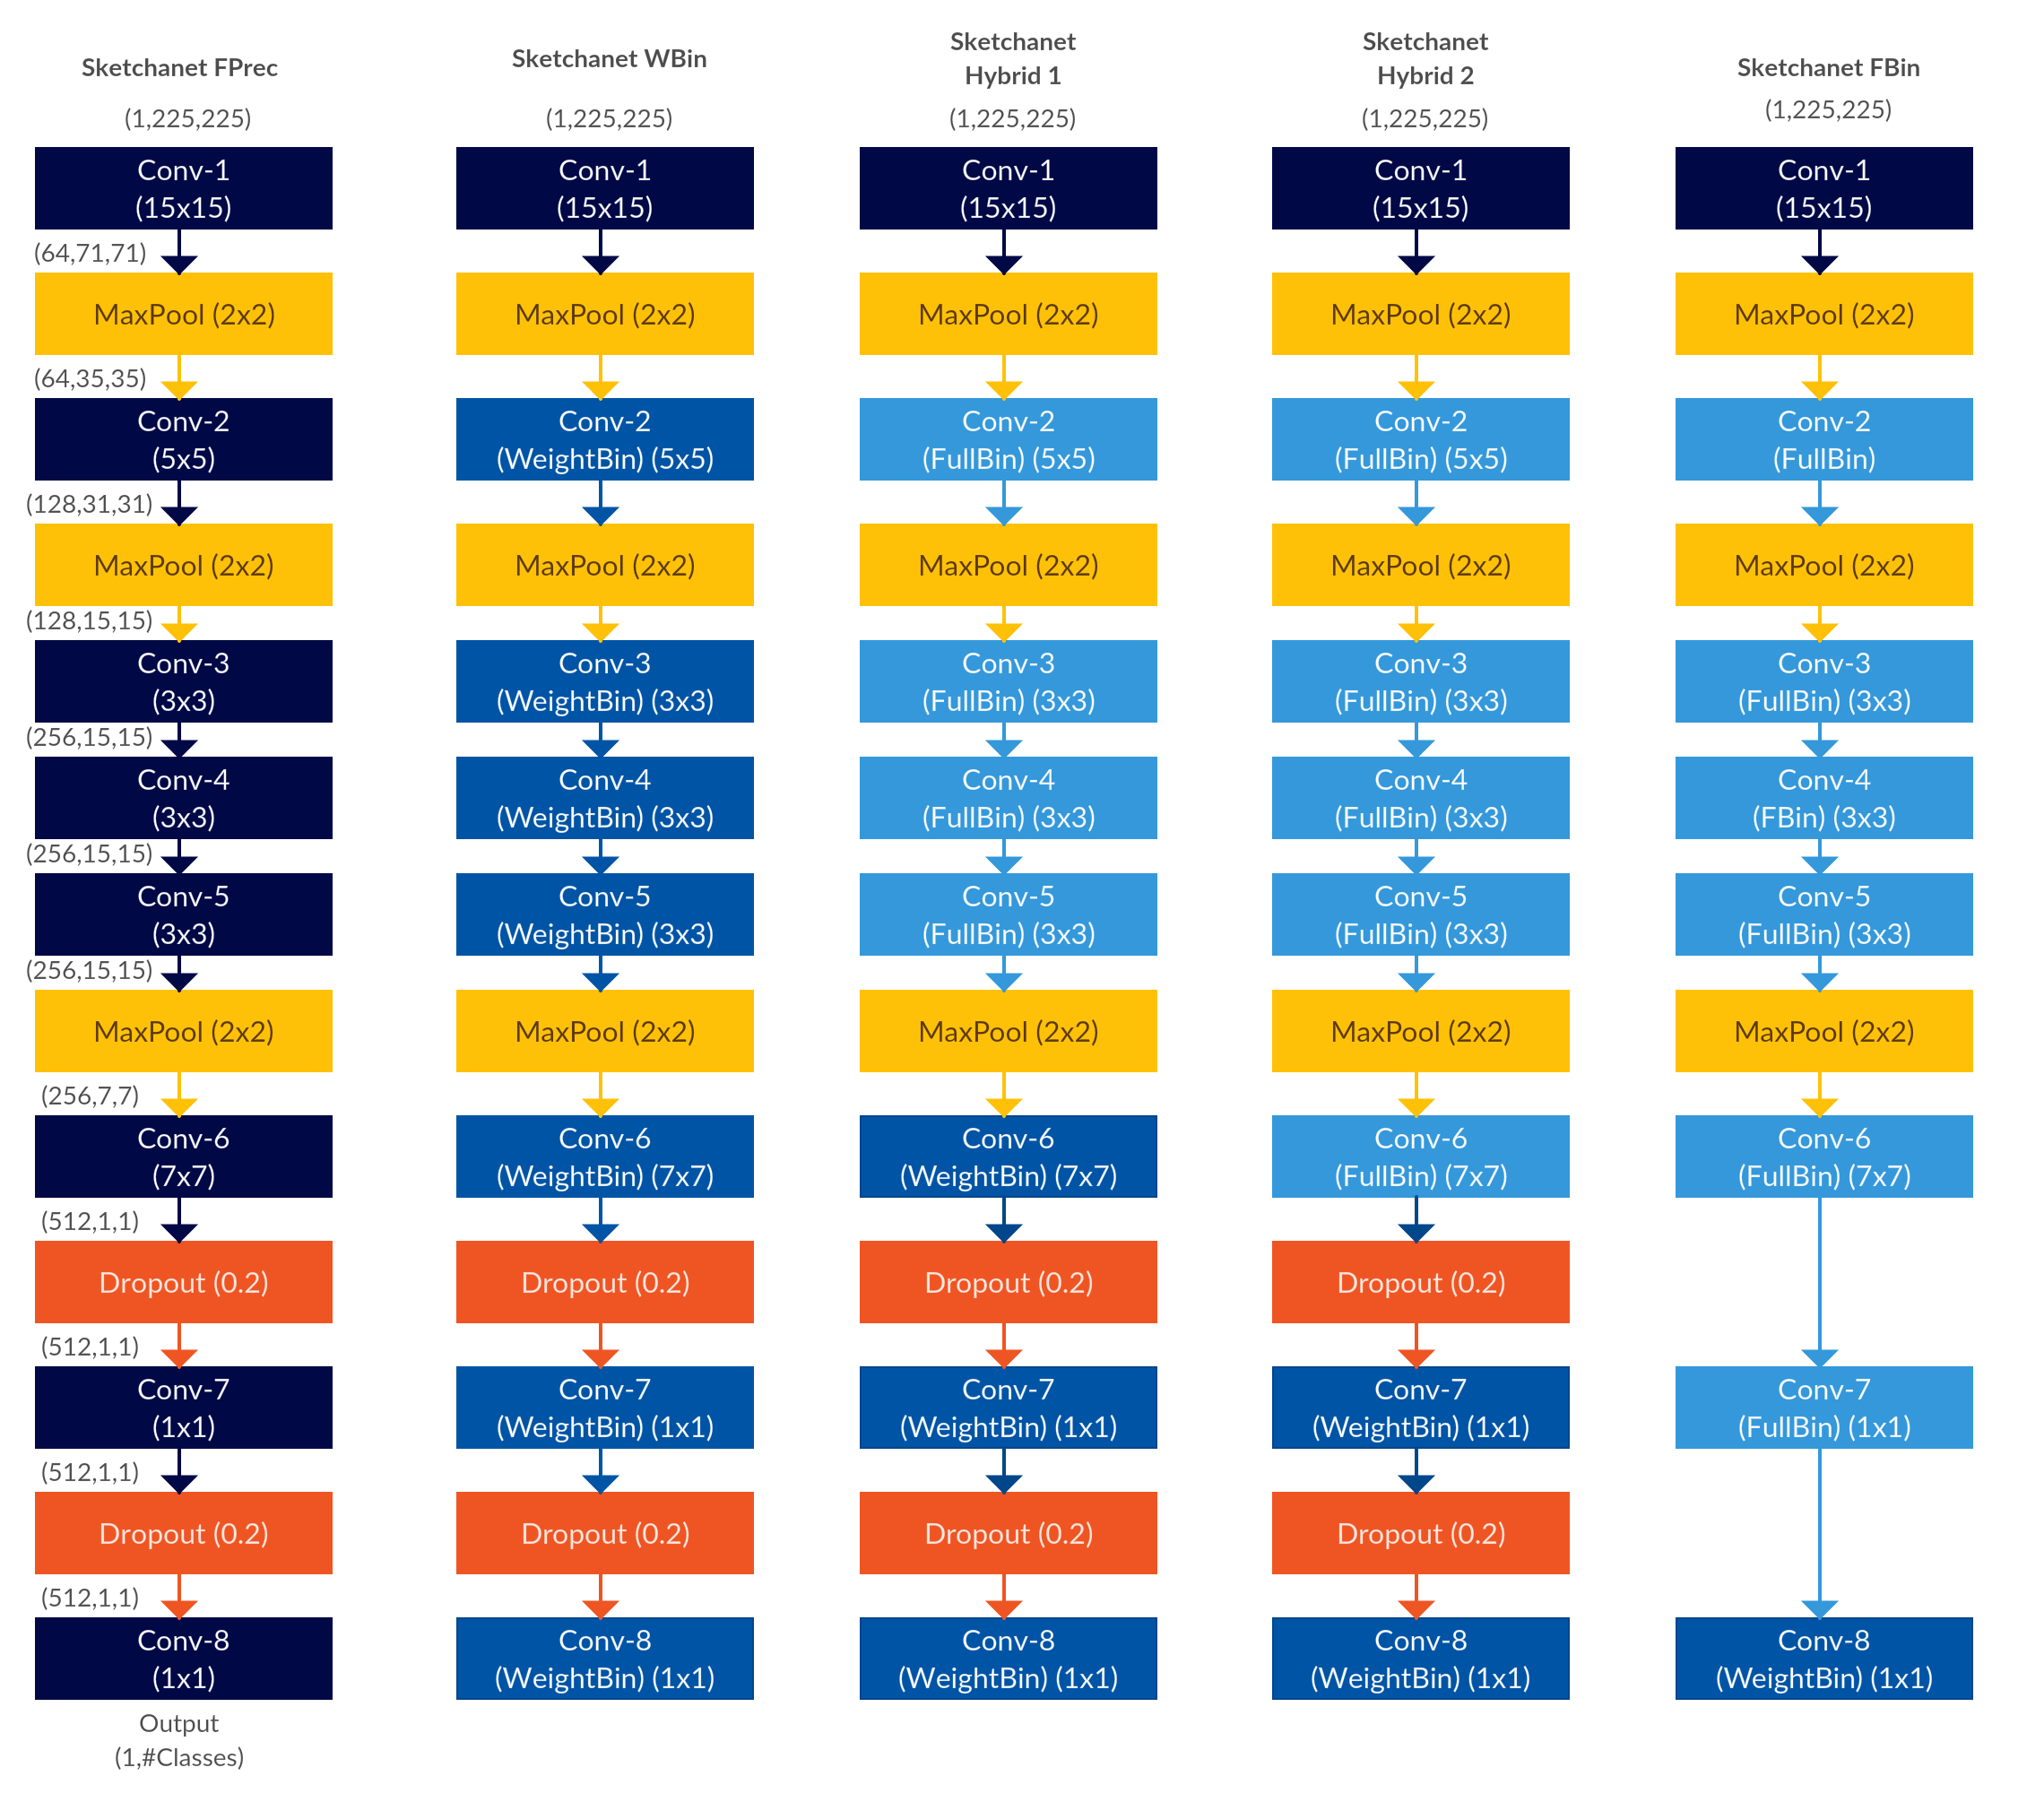
\includegraphics[]{Sketchanet-Final.png}\\
}
\caption{Comparing architectures of FPrec, Wbin, Fbin, and two Hybrid versions of Sketch-A-Net. Our hybrid versions replace most conv layers with FullBinConv layers, but replace layers towards the end with WeightBinConv layers, following the algorithm.}
\vspace*{-0.5cm}
\label{fig:sketchanet}
\end{figure*}

\begin{figure*}[t]
\resizebox{\textwidth}{!}{
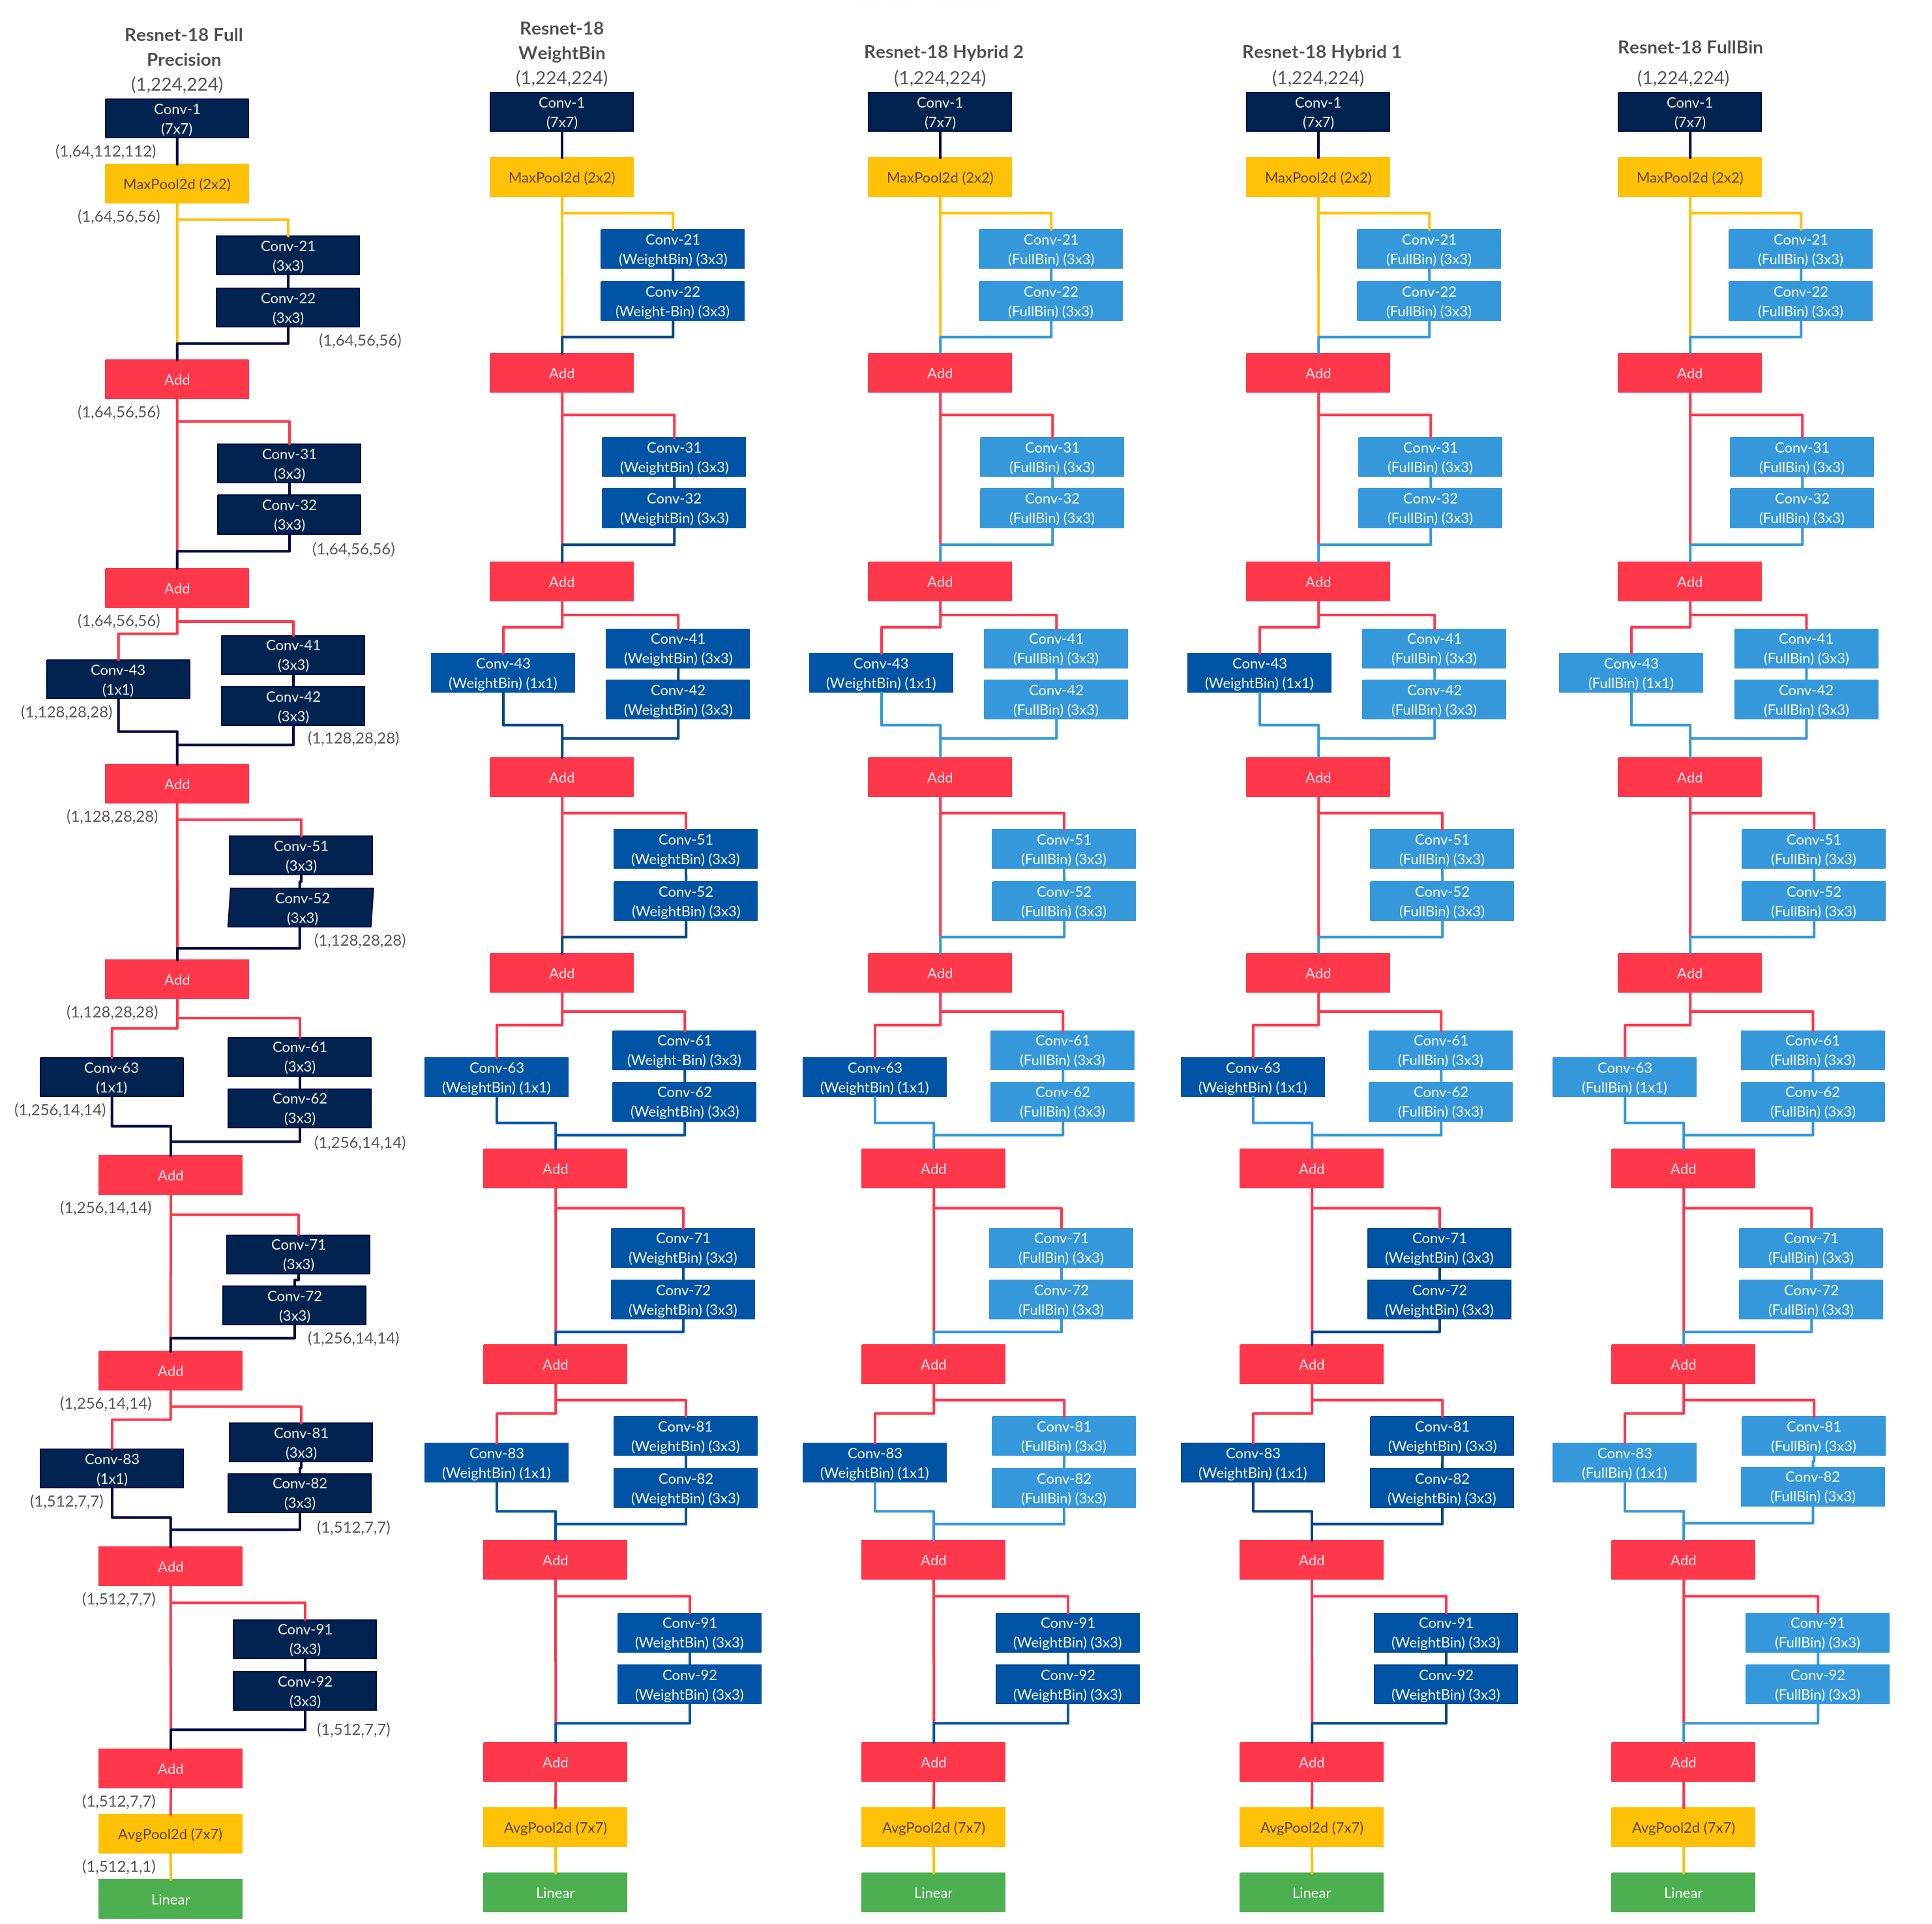
\includegraphics[]{Resnet-Final.png}\\
}
\caption{Comparing architectures of FPrec, Wbin, Fbin, and two Hybrid versions of ResNet-18.}
\label{fig:resnet}
\end{figure*}

\begin{figure*}[t]
\resizebox{\textwidth}{!}{
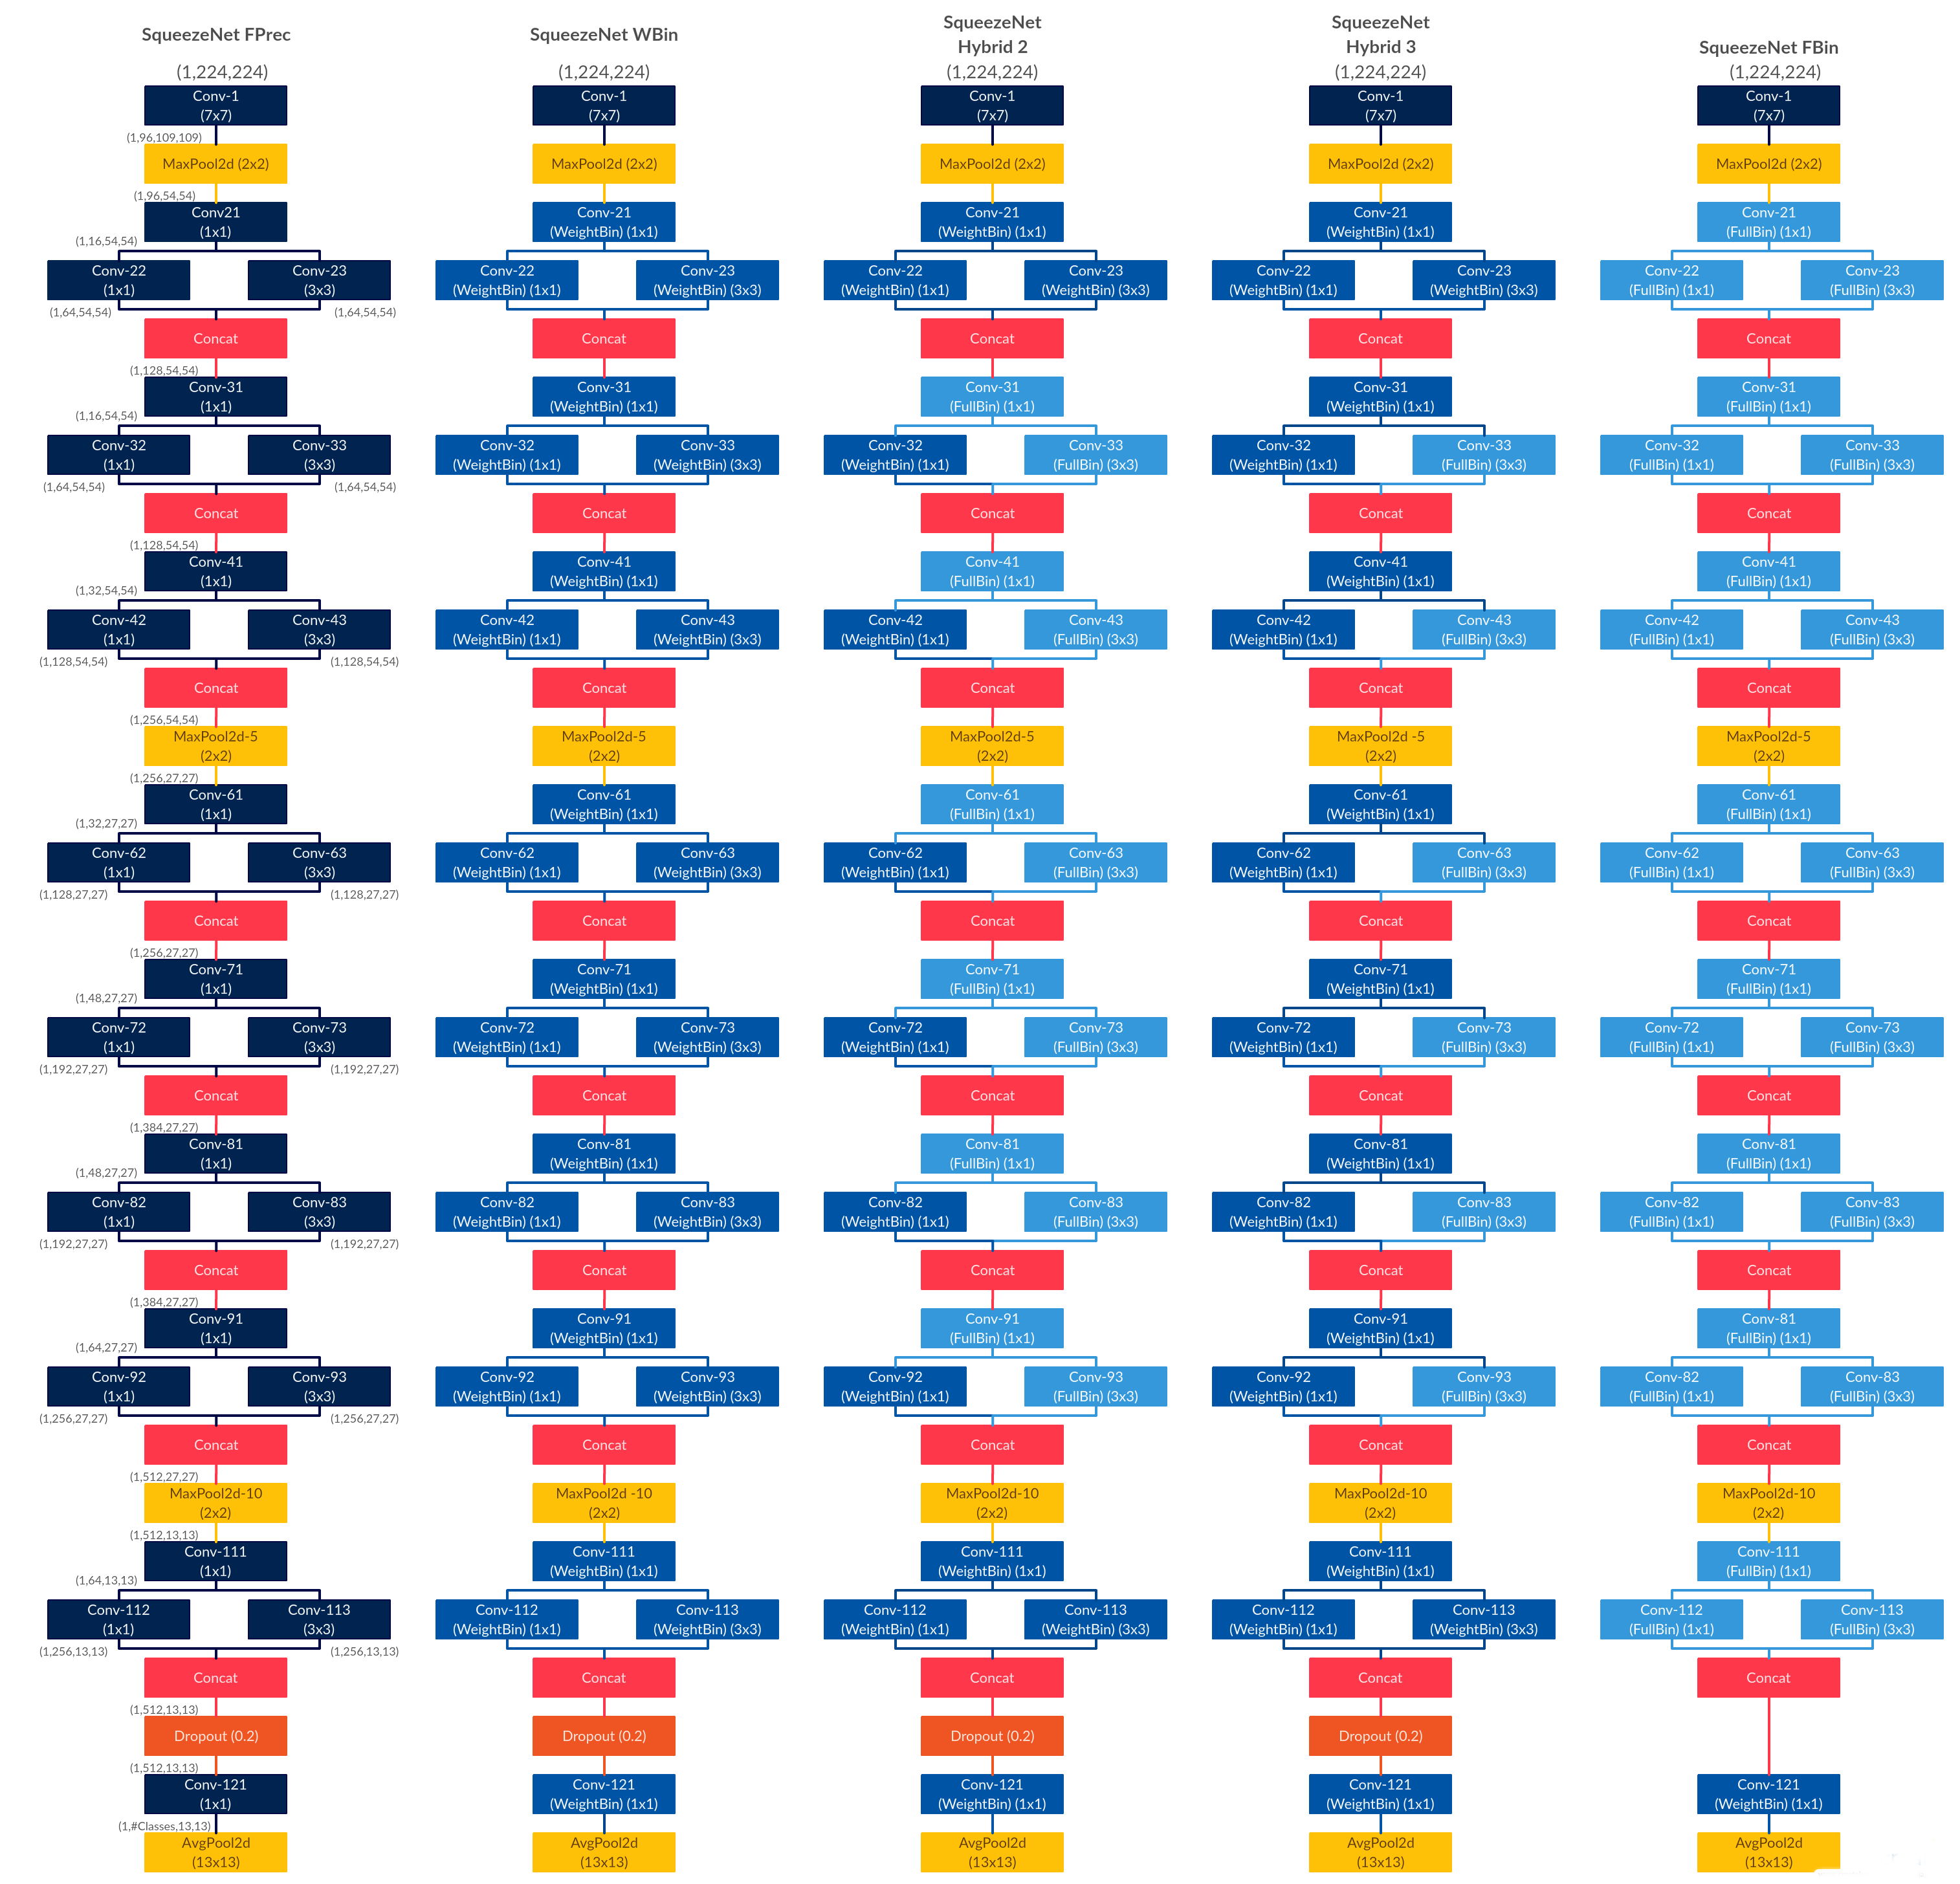
\includegraphics[]{Squeezenet-Final.png}\\
}
\caption{Comparing architectures of FPrec, Wbin, Fbin, and two Hybrid versions of SqueezeNet.}
\label{fig:squeezenet}
\end{figure*}

\begin{figure*}[t]
\resizebox{\textwidth}{!}{
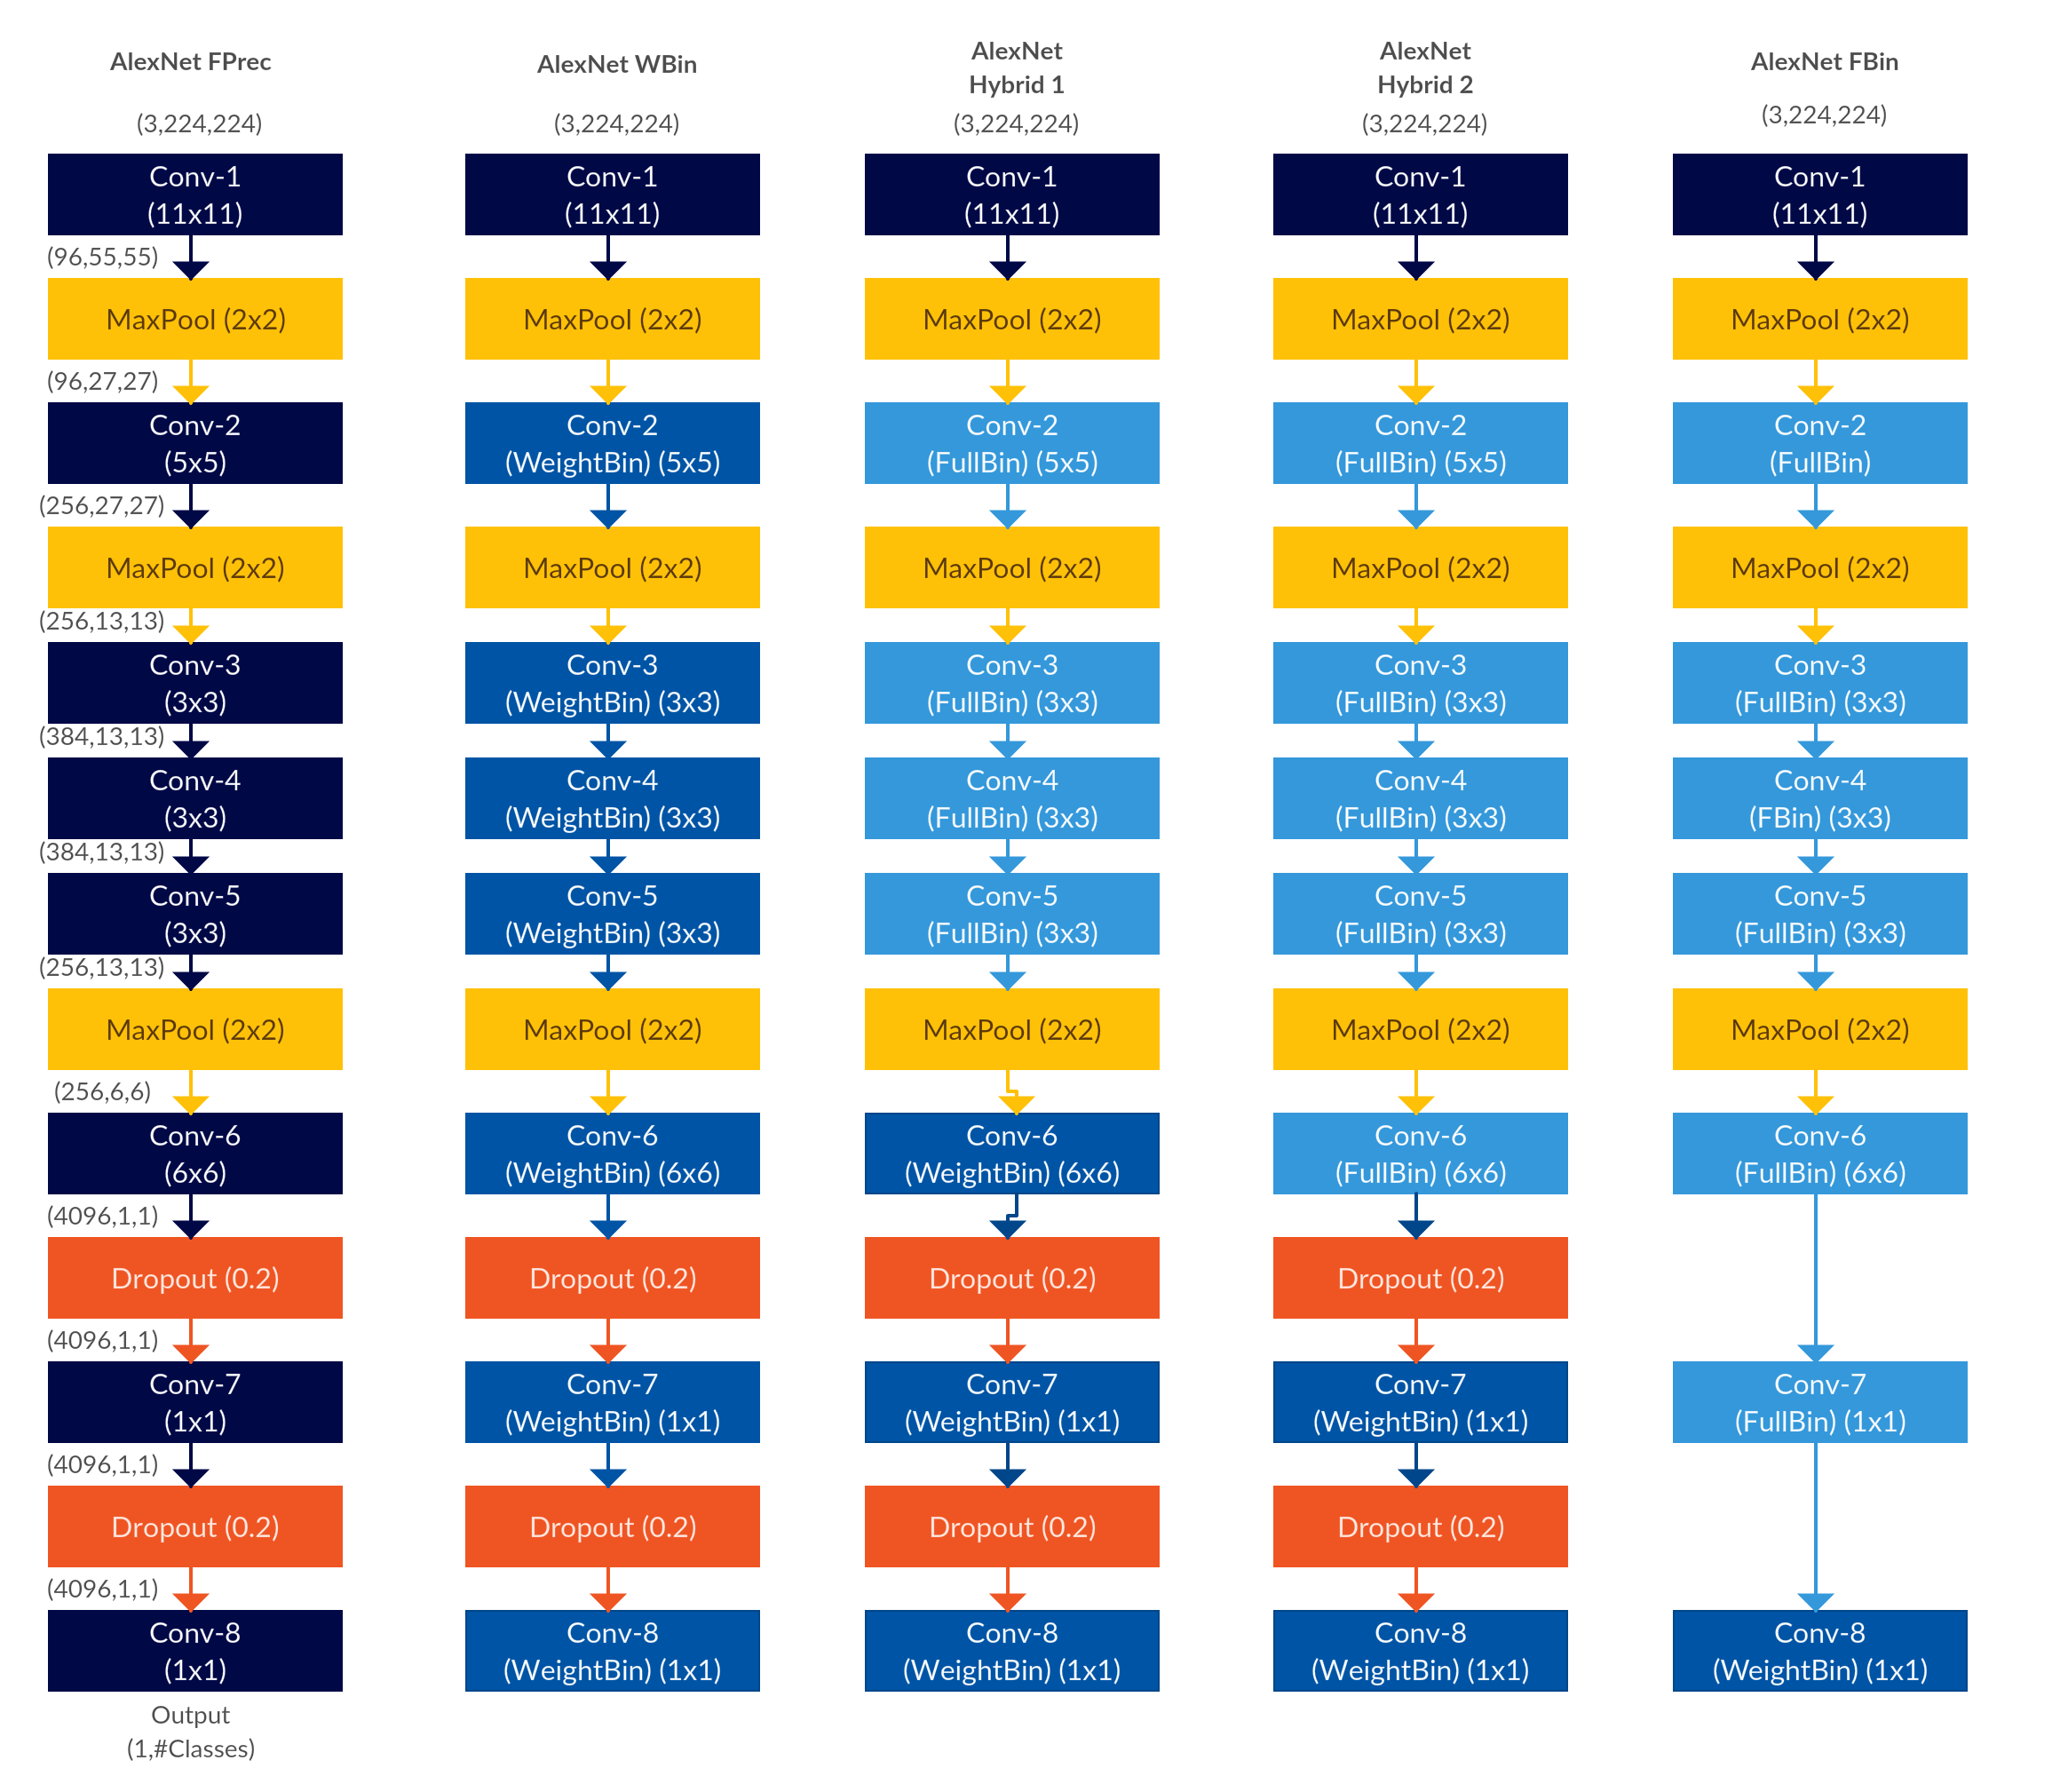
\includegraphics[]{AlexNet-Final.png}\\
}
\caption{Comparing architectures of FPrec, Wbin, Fbin, and two Hybrid versions of AlexNet.}
\label{fig:alexnet}
\end{figure*}

\chapter{Deep Expander Networks: Appendix}
\label{ch:apndx2}

\noindent This part of the appendix provides formal proofs for the theorems stated in Chapter 5 of the thesis. We also include tabulation of results of Figure 3 and 4, alongside additional results that could not be added in the paper due to space constraints.

\section{Explicit Expanders}
\noindent  Many constructions of exmain paperpander graphs have been explored in the past. We will be using a construction that is comparatively easy to describe and implement. We will be considering Cayley graphs, which are obtained from the theory of finite Fields/Groups. The vertex set of such graphs is a group and the edges are defined by addition operation on the vertices. Also we will be describing expanders that are simple undirected graphs. Given an undirected graph $G=(V,E)$, we can obtain  a bipartite expander $G=(V,V',E)$, by making a copy of the vertices $V$ on the other side and adding edges according to $E$.

\subsection{Cayley Expander}
\noindent Let $V$ be a group under an operation $+$ and let $H \subset V$ be a set of generators of the group $V$. The Cayley graph defined by $V,H$ is the graph with vertex set $V$ and the edges $E =\{(x,x+h) : h \in H\}$. For our construction, we will consider the group $\{0,1\}^n$ under coordinate-wise XOR operations. For $H \subset \{0,1\}^n$, the Cayley graph defined by $H$ is $|H|$-regular. It is a well-known result in spectral graph theory that there are set of generators $H$, for which the Cayley graph defined by $\{0,1\}^n, H$ forms an expander with spectral gap $\gamma$.
\begin{theorem}[Alon, Roichman, Proposition 4]
For every $\epsilon$,  there exists explicit $H \subset \{0,1\}^n$ of size $\leq O(n^2/\epsilon^2)$ such that the Cayley graph defined by $\{0,1\}^n, H$ is an expander with spectral gap $\gamma = 1-\epsilon$.
\end{theorem}


\section{Sensitivity in Expanders}
\noindent In this section, we will give details about some properties of expander graphs that are required for proving Theorems 1 and 2. Expander graphs are characterized by the spectral gap, which in turn implies the connectivity properties listed in Section 3.4.\\

\noindent The properties given in Section 3.4 follows from the fact that expanders have a spectral gap. For the sensitivity proofs, we need the following lemmas. The first lemma states that having a spectral gap, implies that all set of vertices of size $\leq n/2$ expands.
\begin{theorem}[Theorem 4.6 \cite{salil2012pseudo}] 
\label{lab:spec}
If $G=(V,E)$ is an expander with spectral gap of $\gamma$ then for every subset $S\subset V$ of size $\leq |V|/2$, the size of the set of neighbors $|N(S)| \geq (1+\gamma) |S|$.
\end{theorem}
The next lemma is known as the expander mixing lemma, deals with the uniform connectivity properties of the expander.
\begin{theorem}[Lemma 4.15 \cite{salil2012pseudo}]
\label{lab:exp-mix-lem}
If $G=(V,E)$ is an $D$-regular expander with spectral gap of $\gamma$ then for every subset $S,T\subset V$,
$$\left| E(S,T) - D \cdot |S| \cdot |T| / n  \right| \leq (1-\gamma)\sqrt{|S| \cdot |T|}$$
where $E(S,T)$ is the set of edges from $S$ to $T$.
\end{theorem}

\noindent In this section, we prove Theorem 1 and Theorem 2 using the properties described above along with the connectivity properties defined in Section 3.1 of the paper.
\begin{theorem}[Sensitivity of X-Nets]\label{thm:conn}
Let $n$ be the number of input as well as output nodes in the network and $G_1,G_2,\cdots, G_t$ be $D$ regular bipartite expander graphs with $n$ nodes on both sides. Then  
every output neuron is sensitive to every input in a Deep X-Linear Network defined by $G_i$'s with depth $t = O( \log n)$.
\end{theorem}
{\bf Proof:} For showing sensitivity, we show that for every pair of input and output $(u,v)$,  there is a path in the X-Net with the $i^{th}$ edge from the $i^{th}$ graph. 
We use the expansion property of the expander graphs. Let $N_1(u)$ be the set of neighbors of $u$ in $G_1$ and $N_i(u)$ be the set of neighbors of $N_{i-1}(u)$ in the graph $G_i$. Since each of the graphs are expanding $|N_{i}(u)| \geq (1+\gamma) \times |N_{i-1}(u)|$, using Lemma \ref{lab:spec}. Since $(1+\gamma) > 1$, we can obtain that for $i = O(\log n)$, $|N_i(u)| \geq n/2$. Similarly we can start from $v$ and define $N_1(v)$ as the set of neighbors of $v$ in $G_t$ and $N_i(v)$ be the set of neighbors of $N_{i-1}(v)$ in the graph $G_{n-i -1}$. Due to the expansion property, for $j = O(\log n)$, $|N_j(v)| \geq n/2$. Now we choose $t = i + j = O(\log n)$ so that the $i^{th}$ graph from $1$ is the same as $j+1^{th}$ graph from $t$. Then we will have that $N_i(u) \cap N_j(v) \neq \phi$. That is there is some vertex in the $i^{th}$ graph that is both connected to $u$ and $v$, which implies that there is a path from $u$ to $v$.

\begin{theorem}[Mixing in Deep Expander Networks]
Let $n$ be the number of input as well as output nodes in the network and $G_1,G_2,\cdots, G_t$ be $D$ regular bipartite expander graphs with $n$ nodes on both sides. Let $S,T$ be subsets of input and output nodes in the X-Linear Network defined by the $G_i$'s. The number of paths between $S$ and $T$ is $\approx D|S||T|/n$
\end{theorem}
{\bf Proof:} First we prove the theorem for the case when $G_1 = G_2 \cdots = G_t = G$. Note that for $t=1$, the theorem is same as the expander mixing lemma (Lemma \ref{lab:exp-mix-lem}). For $t>1$, consider the graph of $t$ length paths denoted by $G^t$. An edge in this graph denotes that there is a path of length $t$ in $G$. Observe that the adjacency matrix of $G^t$ is given by the $t$th power of the adjacency matrix of $G$ and hence the spectral gap of $G^t$, $\gamma_t = \gamma^t$. Now applying the expander mixing lemma on $G^t$ (Lemma \ref{lab:exp-mix-lem}), proves the theorem.\\

\noindent For the case when the graph $G_i$'s are different, let $\gamma_{\min}$ be the minimal spectral gap among the graphs. Since all the graphs are $D$-regular, the largest eigenvector is the all ones vector with eigenvalue $D$ for all the graphs. The eigenvector corresponding to second largest eigenvalue can be different for each graph, but they are orthogonal to the all ones vector. Hence the spectral gap of the $t$ length path graph $G$ is at least $\gamma_{\min}^t$. Finally we apply the expander mixing lemma on $G^t$ to prove the theorem.



\section{Model Details}

\noindent We discuss the model structures in detail, along with tabulated  values of size and flops of various architectures presented as graphs in the main paper. 

\begin{table}[!tbh]
\centering
\resizebox{0.6\columnwidth}{!}{
\begin{tabular}{|l|c|c|c|}
\hline
{\bf AlexNet} & {\bf Filter Shape} & {\bf Filter Shape} & {\bf Filter Shape} \\
\hline
 &  & ({\bf X-AlexNet-1}) & ({\bf X-AlexNet-2})\\
 \hline
Conv2d & 64 x 3 x 11 x 11 & 64 x 3 x 11 x 11 & 64 x 3 x 11 x 11\\
Conv2d & 192 x 64 x 5 x 5 & 192 x 64 x 5 x 5 & 192 x 64 x 5 x 5\\
Conv2d & 384 x 192 x 3 x 3 & 384 x 192 x 3 x 3 & 384 x 192 x 3 x 3\\
Conv2d & 256 x 384 x 3 x 3 & 256 x 384 x 3 x 3 & 256 x 384 x 3 x 3\\
Conv2d & 256 x 256 x 3 x 3 & 256 x 256 x 3 x 3 & 256 x 256 x 3 x 3\\
\hline
Linear & 9216 x 4096 & 1024 x 4096 & 512 x 4096\\
Linear & 4096 x 4096 & 512 x 4096 & 512 x 4096\\
Linear & 4096 x 1000 & 1024 x 1000 & 1024 x 1000\\
\hline
\end{tabular}}
% \vspace{0.1cm}
\caption{Filter sizes for the AlexNet model. Notice the filter sizes of the linear layers of the original model has $|V|\times |U|$ parameters, whereas X-AlexNet models have $|V|\times D$ parameters. Note that $D << |U|$ as stated in Section 3.2. Hence, expander graphs model connections in linear layers (X-Linear) effectively.}
\label{tab:vgg}
\end{table}
\begin{table}[!tbh]
\centering
\resizebox{0.6\columnwidth}{!}{
\begin{tabular}{|l|c|c|c|}
\hline
{\bf VGG} & {\bf Filter Shape} & {\bf Filter Shape} & {\bf Filter Shape}\\
\hline
 &  & ({\bf X-VGG16-1}) & ({\bf X-VGG16-2})\\
 \hline
Conv2d & 64 x 3 x 3 x 3 & 64 x 3 x 3 x 3 & 64 x 3 x 3 x 3\\
Conv2d & 64 x 64 x 3 x 3 & 64 x 64 x 3 x 3 & 64 x 64 x 3 x 3\\
Conv2d & 128 x 64 x 3 x 3 & 128 x 64 x 3 x 3 & 128 x 64 x 3 x 3\\
Conv2d & 128 x 128 x 3 x 3 & 128 x 64 x 3 x 3 & 128 x 64 x 3 x 3\\
Conv2d & 256 x 128 x 3 x 3 & 256 x 32 x 3 x 3 & 256 x 16 x 3 x 3\\
Conv2d & 256 x 256 x 3 x 3 & 256 x 32 x 3 x 3 & 256 x 16 x 3 x 3\\
Conv2d & 256 x 256 x 3 x 3 & 256 x 32 x 3 x 3 & 256 x 16 x 3 x 3\\
Conv2d & 512 x 256 x 3 x 3 & 512 x 32 x 3 x 3 & 512 x 16 x 3 x 3\\
Conv2d & 512 x 512 x 3 x 3 & 512 x 32 x 3 x 3 & 512 x 16 x 3 x 3\\
Conv2d & 512 x 512 x 3 x 3 & 512 x 32 x 3 x 3 & 512 x 16 x 3 x 3\\
Conv2d & 512 x 512 x 3 x 3 & 512 x 32 x 3 x 3 & 512 x 16 x 3 x 3\\
Conv2d & 512 x 512 x 3 x 3 & 512 x 32 x 3 x 3 & 512 x 16 x 3 x 3\\
Conv2d & 512 x 512 x 3 x 3 & 512 x 32 x 3 x 3 & 512 x 16 x 3 x 3\\
\hline
Linear & 512 x 512 & 128 x 512 & 128 x 512\\
Linear & 512 x 10 & 512 x 10 & 512 x 10\\
\hline
\end{tabular}}
% \vspace{0.1cm}
\caption{Filter sizes for the VGG-16 model on CIFAR-10 dataset. The filter sizes given are $|V|\times |U| \times c \times c$ in original VGG network, $|V|\times D \times c \times c$ in our X-VGG16 models. Note that $D << |U|$ as stated in Section 3.2. Hence, expander graphs model connections in Convolutional layers (X-Conv) effectively.}
\label{tab:alexnet}
\end{table}

\begin{table}[!tbh]
\centering
\resizebox{0.6\columnwidth}{!}{
\begin{tabular}{|l|c|c|c|}
\hline
{\bf Model} & {\bf Accuracy} & {\bf \#Params } & {\bf \#FLOPs}\\
\hline
CIFAR10 &  & {\bf(in M)} & {\bf(in 100M)}\\
\hline
X-DenseNetBC-2-40-24 & {\bf 94.83\%} & {\bf 0.4M} & {\bf 1.44}\\
DenseNetBC-40-24 & 94.79\% & 0.7M & 2.88\\
X-DenseNetBC-2-40-36 & 94.98\% & 0.75M & 3.24\\
X-DenseNetBC-2-40-48 & {\bf 95.48\%} & {\bf 1.4M} & {\bf 5.75}\\
DenseNetBC-40-36 & 95.26\% & 1.5M & 6.47\\
X-DenseNetBC-2-40-60 & {\bf 95.71\%} & {\bf 2.15M} & {\bf 8.98}\\
DenseNetBC-40-48 & 95.64\% & 2.8M & 11.50\\
DenseNetBC-40-60 & 95.91\% & 4.3M & 17.96\\
\hline
CIFAR100 &  &  &\\
\hline
X-DenseNetBC-2-40-24 & 74.37\% & 0.4M & 1.44\\
DenseNetBC-40-24 & 76.05\% & 0.7M & 2.88\\
X-DenseNetBC-2-40-36 & {\bf 76.69\%} & {\bf 0.75M} & {\bf 3.24}\\
DenseNetBC-40-36 & 77.84\% & 1.5M & 6.47\\
X-DenseNetBC-2-40-60 & 78.53\% & 2.15M & 8.98\\
X-DenseNetBC-4-70-60 & {\bf 79.56\%} & {\bf 2.6M} & {\bf 10.26}\\
DenseNetBC-40-48 & 79.03\% & 2.8M & 11.50\\
DenseNetBC-40-60 & 79.87\% & 4.3M & 17.96\\
X-DenseNetBC-2-70-60 & 80.89\% & 5.18M & 20.52\\
DenseNetBC-70-60 & 81.28\% & 10.36M & 41.05\\
\hline
\end{tabular}}
% \vspace{0.1cm}
\caption{Results obtained on the state-of-the-art models on CIFAR-10 and CIFAR-100 datasets, ordered by FLOPs per model. X-Nets give significantly better accuracies with corresponding DenseNet models in the same limited computational budget and correspondingly significant parameter and FLOP reduction for models with similar accuracy.}
\label{tab:cifar}
\end{table}
\subsection{Filter structure of AlexNet and VGG}

\noindent In Tables \ref{tab:vgg} and \ref{tab:alexnet}, the detailed layer-wise filter structure is tabulated as stated in Section 5.3 of the paper. We compare the sizes of input channels between the filters, and show that with X-Conv and X-Linear layers, we can train models effectively even with upto 32x and 18x times smaller filters in input dimension in VGG16 and AlexNet models respectively. Hence, modeling connections as weighted adjacency matrix of an Expander graph is an effective method to model connections between neurons, producing highly efficient X-Nets.

\subsection{Results}
\noindent As stated in Section 5.2, Tables \ref{tab:cifar} and \ref{tab:imagenet} presented below give the detailed accuracy, parameters and FLOPs of models displayed in the Figure 3 in the paper. Details of other models are also provided in the same table, which could not be displayed in the paper due to lack of space.\\

\noindent Table \ref{tab:cifar} displays the performance of X-DenseNet models on the CIFAR-10 and CIFAR-100 datasets. If we compare models that have similar number of parameters, we achieve around 0.2\% and 0.6\% increase in accuracy over DenseNet-BC models on CIFAR-10 and CIFAR-100 datasets respectively. In the same manner, we can achieve upto using only two-thirds of the parameter and runtime cost cost respectively, keeping accuracy constant on CIFAR-10 and CIFAR-100 datasets as stated in the paper.\\

\begin{table}[!tbh]
\centering
\resizebox{0.6\columnwidth}{!}{
\begin{tabular}{|l|c|c|c|}
\hline
{\bf Model} & {\bf Accuracy} & {\bf \#Params } & {\bf \#FLOPs}\\
\hline
ResNet &  & {\bf(in M)} & {\bf(in 100M)}\\
\hline
X-ResNet-2-34 & 69.23\% & 11M & 35\\
X-ResNet-2-50 & {\bf 72.85\%} & {\bf 13M} & {\bf 40}\\
ResNet-34 & 71.66\% & 22M & 70\\
X-ResNet-2-101 & {\bf 74.87\%} & {\bf 22.5M} & {\bf 80}\\
ResNet-50 & 74.46\% & 26M & 80\\
ResNet-101 & 75.87\% & 45M & 160\\
\hline
DenseNetBC &  &  & \\
\hline
MobileNet \cite{howard2017mobilenets} & 70.6\% & 4.2M & 5.7 \footnote{These are reported as mult-add operations} \\
ShuffleNet \cite{zhang2018shufflenet} & 70.9\% & 5M & 5.3 \footnote{These are reported as mult-add operations} \\
X-DenseNetBC-2-121 & {\bf 70.5\%} & {\bf 4M} & 28\\
X-DenseNetBC-2-169 & 71.7\% & 7M & 33\\
X-DenseNetBC-2-201 & 72.5\% & 10M & 43\\
X-DenseNetBC-2-161 & {\bf 74.3\%} & 14.3M & {\bf 55}\\
DenseNetBC-121 & 73.3\% & 8M & 55\\
DenseNetBC-169 & 74.8\% & 14M & 65\\
DenseNetBC-201 & 75.6\% & 20M & 85\\
DenseNetBC-161 & 76.3\% & 28.5M & 110\\
\hline
\end{tabular}}
% \vspace{0.1cm}
\caption{Results obtained on the state-of-the-art models on ImageNet dataset, ordered by FLOPs. We also observe that X-DenseNetBC models outperform ResNet and X-ResNet models in both compression, parameters and FLOPs and achieve comparable accuracies with the highly efficient MobileNets and ShuffleNets in the same parameter budget, albeit with much higher FLOPs due to architectural constraints.}
\label{tab:imagenet}
\end{table}

\noindent Similarly, Table \ref{tab:imagenet} displays the performance of X-ResNet and X-DenseNet models on the ImageNet datasets. We can observe that we achieve around 3.2\% and 1\% increase in accuracy over ResNet and DenseNet-BC models in the same computational budget. Also, we can observe that we require approximately 15\% less FLOPs for achieving similar accuracies over DenseNet models and 15\% less parameters for achieving similar accuracies over the ResNet model respectively as stated in the paper. We also observe that X-DenseNetBC models outperform ResNet and X-ResNet models in both compression, parameters and FLOPs and achieve comparable accuracies with MobileNets \cite{howard2017mobilenets} and ShuffleNets \cite{zhang2017shufflenet} in the same parameter budget, albeit with much higher computational cost due to architectural constraints. \\

\begin{table}[!tbh]
\centering
\resizebox{0.6\columnwidth}{!}{
\begin{tabular}{|l|c|c|c|}
\hline
{\bf Model} & {\bf Accuracy} & {\bf \#Params } & {\bf \#FLOPs}\\
\hline
Wider & & {\bf(in M)} & {\bf(in 100M)} \\
\hline
DenseNetBC-40-60 & 79.87\% & 4.3M & 17.96\\
X-DenseNetBC-2-40-60 & 78.53\% & 2.15M & 8.98\\
X-DenseNetBC-4-40-60 & 77.54\% & 1.08M & 4.49\\
X-DenseNetBC-8-40-60 & 75.29\% & 0.54M & 2.24\\
X-DenseNetBC-16-40-60 & 74.44\% & 0.27M & 1.12\\
\hline
DenseNetBC-40-100 & 80.9\% & 11.85M & 49.85\\
X-DenseNetBC-4-40-100 & 78.87\% & 2.9M & 12.46\\
X-DenseNetBC-8-40-100 & 77.75\% & 1.48M & 6.23\\
X-DenseNetBC-16-40-100 & 76.2\% & 0.74M & 3.12\\
\hline
DenseNetBC-40-200 & 81.62\% & 47.19M & 199.28\\
X-DenseNetBC-4-40-200 & 80.66\% & 11.79M & 49.82\\
X-DenseNetBC-10-40-200 & 79.46\% & 4.71M & 19.93\\
X-DenseNetBC-20-40-200 & 78.33\% & 2.3M & 9.96\\
X-DenseNetBC-30-40-200 & 77.29\% & 1.6M & 6.64\\
X-DenseNetBC-50-40-200 & 75.7\% & 0.9M & 3.99\\
X-DenseNetBC-80-40-200 & 73.26\% & 0.5M & 2.49\\
\hline
Deeper &  &  &\\
\hline
DenseNetBC-40-60 & 79.87\% & 4.3M & 17.96\\
X-DenseNetBC-2-40-60 & 78.53\% & 2.15M & 8.98\\
X-DenseNetBC-8-40-60 & 77.54\% & 0.54M & 2.24\\
X-DenseNetBC-16-40-60 & 75.29\% & 0.27M & 1.12\\
\hline
DenseNetBC-58-60 & 80.79\% & 7.66M & 30.96\\
X-DenseNetBC-2-58-60 & 80.29\% & 3.83M & 15.48\\
X-DenseNetBC-4-58-60 & 78.74\% & 1.9M & 7.74\\
X-DenseNetBC-8-58-60 & 77.98\% & 0.95M & 3.87\\
X-DenseNetBC-16-58-60 & 75.87\% & 0.47M & 1.93\\
\hline
DenseNetBC-70-60 & 81.28\% & 10.36M & 41.05\\
X-DenseNetBC-2-70-60 & 80.89\% & 5.18M & 20.52\\
X-DenseNetBC-4-70-60 & 79.56\% & 2.6M & 10.26\\
X-DenseNetBC-8-70-60 & 77.48\% & 1.3M & 5.13\\
X-DenseNetBC-16-70-60 & 77.23\% & 0.65M & 2.57\\
\hline
\end{tabular}}
% \vspace{0.1cm}
\caption{We display accuracies, parameters and FLOPs of all the wider and deeper networks on CIFAR-100 listed in increasing compression order. This proves that efficiently designing layers like X-Conv and X-Linear allows us to train wider and deeper networks frugally.}
\label{tab:ultranets}
\end{table}

\noindent Table \ref{tab:ultranets} displays accuracies, parameters and FLOPs of all the wider and deeper networks trained on CIFAR-100 dataset as discussed in Section 5.4. They are listed in increasing compression order from DensenetBC (1x) to the highest compressed X-DenseNet. The figure indicates that Expander Graphs modeling can scale up to high compression ratios without drastic drops in accuracies, enabling us to train deeper and wider networks retaining similar FLOPs and parameters effectively. We believe this modeling can open up a interesting exploration of training significantly deeper and wider range of models, unlike the current compression techniques as X-Nets are highly compressed networks since definition. 

\subsection{Experimental Details}
\label{sec:expdetails}
\noindent To ensure better reproducibility, we used the same hyper-parameters, models, training schedules and dataset structures from the official \href{https://github.com/pytorch/examples/blob/master/imagenet/main.py}{PyTorch repository} for ResNet and DenseNet-BC ImageNet experiments. Similarly, we followed the \href{https://github.com/marvis/pytorch-mobilenet}{pytorch-mobilenet repository} including all hyperparameters for all the mobilenet experiments. Likewise, we followed the \href{https://github.com/andreasveit/densenet-pytorch/}{densenet-pytorch repository} by Andreas Veit for all DenseNet-BC experiments on CIFAR-10/100 datasets, and the \href{https://github.com/chengyangfu/pytorch-vgg-cifar10}{pytorch-vgg-cifar10} repository by Cheng-Yang Fu for VGG16 experiments on the CIFAR-10 dataset. We deleted a linear layer and remove dropouts from the VGG16 model. There were two differences between our code and the PyTorch ImageNet repository. Our ImageNet training code used a compressed version of Imagenet with images resized to 256x256, we used a batchsize of 128 for all experiments, hence typically results in slightly lower accuracies. Our AlexNet model used BatchNorm layers to stabilize training, with a batchsize of 384.\\

\noindent We trained all the models on a setup consisting of 10 Intel Xeon E5-2640 cores and 2 GeForce GTX 1080 Ti GPUs. All networks are trained from scratch. We modeled connections as  random expanders for all experiments. The X-Conv layers did not have a bias. No dropouts were used. Additional details regarding all models, accuracies, and numbers of parameters and FLOPs is tabulated in the supplementary material for reference due to lack of space. \\ 

\noindent All models in the plot were trained from the ImageNet code available on Pytorch Official repository including the original DenseNet and ResNet models. Note that this training code is common for all models in the repository and not fine-tuned to any specific model like ResNet or DenseNet. Hence the accuracies we report is slightly lower that those reported using model-specific training code. However, note that we have used the same code for training both the original models and the expander versions of these models. Hence the comparison is a fair one. Same is true with the  AlexNet model. Note that we use the original AlexNet architecture, and not CaffeNet. \\

\noindent In contrast, training with fine-tuned code is expected to give a 1-2\% improvement over MobileNets in Table \ref{tab:imagenet}. Training schedules suited to X-Nets, hyper-parameter tuning, Activation layers tailored to X-Nets could further improve the accuracies. Overall, we believe that investigating training methods for X-Nets has a lot of potential for improving their performance.

%--------------------------------------------------------

%--------------------------------------------------------
\bibliographystyle{latex8}
\bibliography{./sampleBib}

\end{document}
